\documentclass[a4paper]{report}

\input{setup/preamble}
\input{setup/macros}
\input{setup/letterfonts}
\usepackage{placeins} % Package to handle floating elements

\addbibresource{gr.bib} 

\course{Topic in Econometrics}
\professor[https://markomlikota.github.io/]{Marko Mlikota}
\me[jingle.fu@graduateinstitute.ch]{}
\institute{Graduate Institute of International and Developoment Studies, Geneva}
\class{International Economics}
\session{Semester III, 2025}
\date{Based on lectures by \profloc{} in Spring semester, 2025
% \\ Notes created by Mubtasim Fuad 
\\~\\ Draft updated on \today}

\begin{document}

\renewcommand\thepage{Title}
\maketitle
\renewcommand\thepage{Preface} 
% \chapter*{Preface}  % to show preface on toc
\begin{myminipage} 
     This is the lecture note taken in the course \textit{\courseloc} taught by \profloc{} at \instituteloc{} as part of the \classloc{} program (\sessionloc).
     
     Currently, these are just drafts of the lecture notes. There can be typos and mistakes anywhere. So, if you find anything that needs to be corrected or improved, please inform at \myemailloc. \bigskip

     % I am deeply grateful to my late friend, Gilles Castel, who introduced me to \LaTeX{} for the first time.
\end{myminipage}

% \addcontentsline{toc}{chapter}{\protect\numberline{}Preface} % to show preface on toc
\pagenumbering{gobble}
% \pagenumbering{roman}   % to show preface on toc
\newpage
\pagestyle{plain}
\pagenumbering{roman}
\pdfbookmark{\contentsname}{toc}              
\setcounter{tocdepth}{3}
\tableofcontents
\newpage
\pagestyle{head}
\pagenumbering{arabic}

% start lectures
\chapter{Introduction to Bayesian Econometrics}
\section{Introduction}

\begin{definition}[Proportional Function]
    We say $f(x)$ is proportional to $g(x)$ if there exists a constant $c$,
    such that $f(x) = c \cdot g(x)$ for all $x$ in the domain of interest.
    We denote this relationship as $f(x) \propto g(x)$.
\end{definition}

If $y$ is a R.V. with pdf $f(y) \propto \exp(-\lambda y)$ for $y \geq 0$ and $0$ otherwise,
then we know $f(y) = c \cdot \exp(-\lambda y)$.
To find $c$, we use the fact that the total probability must equal 1:
\begin{equation}
    \int_0^\infty f(y) dy = 1 \implies \int_0^\infty c \cdot \exp(-\lambda y) dy = 1
\end{equation}
Calculating the integral, we have:
\begin{equation}
    c \cdot \left[ -\frac{1}{\lambda} \exp(-\lambda y) \right]_0^\infty = 1
\end{equation}
Evaluating the limits, we get:
\begin{equation}
    c = \lambda 
\end{equation}

Now looking at the normal distribution: $y \sim \mathcal{N} \left( \mu , \sigma^2 \right)$
we have
\begin{align}
    p(y | \mu, \sigma^2) &= \frac{1}{\sqrt{2 \pi \sigma^2}} \exp \left( -\frac{(y - \mu)^2}{2\sigma^2} \right) \\
    & \propto \exp \left( -\frac{1}{2\sigma^2} (y - \mu)^2 \right)
\end{align}

For a simple linear regression model $y_i = \theta + u_i$, where $\mathbb{E}[ u_i | \theta =0]$,
we know $\mathbb{E}[ y_i | \theta ] = \theta$.



\begin{itemize}
    \item Least-squares estimator:
    \begin{align}
        \hat{\theta}_{LS} &= \arg \min_\theta \sum_{i=1}^n (y_i - \mathbb{E}[ y_i | \theta ])^2 \\
        &= \arg \min_\theta \left( y_i - \theta \right)^2 \\
        &= \frac{1}{n} \sum_{i=1}^n y_i
    \end{align}
    \item Maximum likelihood estimator(Assuming $y_i | \theta \sim \mathcal{N} \left( \theta , \sigma^2 \right)$):
    \begin{align}
        \hat{\theta}_{ML} &= \arg \max_\theta \prod_{i=1}^n p(y_i | \theta) \\
        &\propto \arg \max_\theta \prod_{i=1}^n \exp \left( -\frac{1}{2\sigma^2} (y_i - \theta)^2 \right) \\
        &\propto \arg \min_\theta \sum_{i=1}^n (y_i - \theta)^2 \\
        &= \frac{1}{n} \sum_{i=1}^n y_i = \hat{\theta}_{LS}
    \end{align}
    It's easy to see that:
    \begin{align}
        \mathbb{E}[\hat{\theta } | \theta ] &= \mathbb{E} \left[ \frac{1}{n} \sum_{i=1}^n y_i | \theta \right] = \theta \\
        \mathbb{V}[\hat{\theta } | \theta ] &= \mathbb{V} \left[ \frac{1}{n} \sum_{i=1}^n y_i | \theta \right] = \frac{\sigma^2}{n}
    \end{align}
    Even without assuming that $\hat{\theta } | \theta \sim \mathcal{N} \left( \theta , \frac{\sigma^2}{n} \right)$,
    we know by the Central Limit Theorem that:
    \begin{equation}
        \sqrt{n} \left( \hat{\theta } - \theta \right) \xrightarrow{d} \mathcal{N} \left( 0 , \sigma^2 \right) \Rightarrow \hat{\theta } | \theta \sim \mathcal{N} \left( \theta , \frac{\sigma^2}{n} \right)
    \end{equation}
\end{itemize}

\begin{definition}[Posterior]
    The posterior distribution of a parameter $\theta$ given data $y$ is defined as:
    \begin{equation}
        p(\theta | y) = \frac{p(y | \theta) p(\theta)}{p(y)} \propto p(y | \theta) p(\theta)
    \end{equation}
    where $p(y | \theta)$ is the likelihood, $p(\theta)$ is the prior distribution of $\theta$, and $p(y)$ is the marginal likelihood.

    This shows how, given a prior belief about $\theta$ and observed data $y$,
    we can update our belief to form the posterior distribution.
\end{definition}

\begin{eg}
    Taking a simple example: 
    \begin{equation}
        y_i | \theta \sim \mathcal{N} \left( \theta , 1 \right) \Rightarrow p(y_i | \theta) = \frac{1}{\sqrt{2\pi}} \exp \left( -\frac{1}{2} (y_i - \theta)^2 \right)
    \end{equation}
    Suppose $\theta \sim \mathcal{N} \left( \theta , \frac{1}{\lambda } \right)$.
    \begin{align}
        p(\theta | y) & \propto p(y | \theta) p(\theta) \\
        &= (2\pi )^{ -\frac{n}{2}} \exp \left( -\frac{1}{2} (y_i - \theta)^2 \right) \cdot \frac{1}{\sqrt{2\pi \frac{1}{\lambda}}} \exp \left( -\frac{1}{2 \frac{1}{\lambda }} (\theta - \theta_0)^2 \right) \\
        & \propto \exp \left( -\frac{1}{2} \sum_{i=1}^n (y_i - \theta)^2 - \frac{\lambda }{2} (\theta - \theta_0)^2 \right) \\
        & \propto \exp \left( -\frac{1}{2} \left[ (n + \lambda ) \theta^2 - 2 \left(\sum_{i=1}^n y_i + \lambda \theta_0\right) \theta \right] \right) \\
        \theta | y & \sim \mathcal{N} \left( \frac{1}{n + \lambda } \left( \sum_{i=1}^n y_i + \lambda \theta_0 \right), \frac{1}{n + \lambda } \right)
    \end{align}
    We guess that $\theta | y \sim \mathcal{N} \left( \bar{\theta }, \bar{V} \right)$,
    then we can write:
    \begin{align}
        p \left( \theta | y \right) & \propto \exp \left( -\frac{1}{2} \bar{V}^{-1} (\theta - \bar{\theta })^2 \right) \\
        & \propto \exp \left( -\frac{1}{2} \left[ \bar{V}^{-1} \theta^2 - 2 \bar{V}^{-1} \bar{\theta } \theta \right] \right)
    \end{align}
    then, we know that:
    \begin{equation}
        \bar{V}^{-1} = n + \lambda 
    \end{equation}
    and
    \begin{align}
        \bar{\theta } &= \frac{1}{n + \lambda } \left( \sum_{i=1}^n y_i + \lambda \theta_0 \right) \\
        &= \frac{1}{n + \lambda } \cdot \left[ n \cdot \sum_{i=1}^n y_i + \lambda\, \theta_0 \right] \\
        & \to \begin{cases}
            \theta_0, &\text{ if } \lambda \to \infty ; \\
            \hat{\theta }, &\text{ if } \lambda \to 0 \text{ and/or } n \to \infty .
        \end{cases}
    \end{align}
    In general, we can push $\theta _0$ to $0$ by re-centering $y_i$.
    Then we have:
    \begin{equation}
        \hat{\theta } = \frac{n}{n + \lambda }\, \underset{ \hat{\theta }_{ML} }{ \underbrace{ \frac{1}{n} \sum_{i=1}^n y_i }}
    \end{equation}
    then,
    \begin{align}
        \mathbb{E}[\hat{\theta } | \theta ] &= \mathbb{E}\left[ \frac{1}{n + \lambda} \sum_{i=1}^n y_i | \theta \right] \\
        &= \frac{1}{n + \lambda} \sum_{i=1}^n \mathbb{E}[y_i | \theta ] = \frac{1}{n + \lambda} \sum_{i=1}^n \theta = \frac{n}{n + \lambda} \theta 
    \end{align}
    for any $\lambda > 0$, this $\hat{\theta }$ is biased.
    \begin{align}
        \mathbb{V}[\hat{\theta } | \theta ] &= \mathbb{V}\left[ \frac{1}{n + \lambda} \sum_{i=1}^n y_i | \theta \right] \\
        &= \frac{1}{(n + \lambda)^2} \sum_{i=1}^n \mathbb{V}[y_i | \theta ] \\
        &= \frac{n}{(n + \lambda)^2} \\
        &< \frac{1}{n} = \mathbb{V}[\hat{\theta }_{ML} | \theta ] \text{ for any } \lambda > 0.
    \end{align}
\end{eg}

\section{Hypothesis Testing}

We want to test $H_0: \theta = 0$ vs $H_1: \theta \neq 0$.
$\varphi \in \{0, 1\}$ is a test function, where $\phi = 1$ means accept,
then the size of the test is defined as:
\begin{equation}
    \alpha = \mathbb{P}(\varphi = 1 | \theta = 0) = \mathbf{1} \{\theta < \theta_0 \}
\end{equation}

We have:
\begin{align}
    \mathbb{P}(\theta | y) \begin{dcases}
        p\left( \theta \in \Theta_0 | y \right);\\
        p\left( \theta \notin \Theta_0 | y \right) = 1 - p\left( \theta \in \Theta_0 | y \right).
    \end{dcases}
\end{align}
Then, the posterior odds ratio is defined as:
\begin{equation}
    \frac{p\left( \theta \in \Theta_0 | y \right)}{p\left( \theta \in \Theta_1 | y \right)} = \frac{p\left( \theta \in \Theta_0 | y \right)}{1 - p\left( \theta \in \Theta_0 | y \right)}
\end{equation}
The Bayes factor is defined as:
\begin{equation}
    BF = \frac{\text{Post. Odds}}{\text{Prior Odds}}
\end{equation}

\begin{eg}
    
Suppose $\theta \in \{0, 1\}$, and $y | \theta \in \{ 0,1,2,3,4 \}$,
\begin{table}[H]
    \centering
    \begin{tabular}{c|ccccc}
        \toprule
         & 0 & 1 & 2 & 3 & 4 \\
        \midrule
        $p(y | \theta = 0)$ & 75\% & 14\% & 4\% & 3.7\% & 3.3\% \\
        $p(y | \theta = 1)$ & 70\% & 25.1\% & 4\% & 0.5\% & 0.4\% \\
        \bottomrule
    \end{tabular}
    \caption{Example}
    \label{tab:example}
\end{table}

Suppose $y=2$, then the hypothesis test results are:
\begin{align}
    \mathcal{H}_0: \theta = 0 & \to p(y \geq 2 | \theta = 0) = 11\% \\
    \mathcal{H}_1: \theta = 1 & \to p(y \geq 2 | \theta = 1) = 4.9\%
\end{align}

The Bayes factors are:
\begin{align}
    BF &= \frac{p\left(\theta = 1 | y = 2 \right)}{p\left(\theta = 0 | y = 2 \right)} \\
    &= \frac{p(y = 2 | \theta = 1)p(\theta = 1)}{p(y = 2 | \theta = 0)p(\theta = 0)}
\end{align}

\end{eg}

Consider $c(y)$ such that $\mathbb{P}\left[ \theta \in c(y) | \theta \right] = 1- \alpha $, e.g. 95\%,
then the decision rule is:
\begin{equation}
    \left\{ \theta_0 \in \Theta : \varphi(\theta_0, \alpha ) = 1 \right\}
\end{equation}
Under Bayesian approach, we say:  $\mathbb{P}\left[ \theta \in c(y) | y \right] = 1- \alpha $, e.g. 95\%,
then we have the Highest Posterior Density(HPD) region:
\begin{equation}
    c(y) = \left\{ \theta : p(\theta | y) \geq k_\alpha  \right\}
\end{equation}
where $k_\alpha $ is such that $\mathbb{P}\left[ \theta \in c(y) | y \right] = 1- \alpha $.

\begin{figure}[ht]
    \centering
    \begin{tikzpicture}
        \pgfmathsetmacro{\mu}{0.3}      % posterior mean
        \pgfmathsetmacro{\sigma}{0.6}   % posterior sd
        \pgfmathsetmacro{\peak}{1/(sqrt(2*pi)*\sigma)}
        \pgfmathsetmacro{\kfactor}{0.42} % k_alpha as fraction of peak (adjust for illustration)
        \pgfmathsetmacro{\kval}{\kfactor*\peak}
        \begin{axis}[
            width=0.8\linewidth,
            height=5.2cm,
            domain=\mu-3*\sigma:\mu+3*\sigma,
            samples=200,
            axis x line=middle,
            axis y line=left,
            xlabel={\(\theta\)},
            ylabel={\(p(\theta\mid y)\)},
            xmin=\mu-2.2,
            xmax=\mu+2.2,
            ymin=0,
            ytick=\empty,
            enlargelimits=false,
            tick align=outside,
            clip=false,
            ]
            % posterior density path
            \addplot[name path=post, very thick, smooth, blue] 
                {1/(sqrt(2*pi)*\sigma)*exp(-0.5*((x-\mu)/\sigma)^2)};
            % horizontal k line
            \addplot[name path=kline, draw=none] {\kval};
            % fill HPD region (where posterior >= k)
            % we use a soft clip range that contains the two intersections for clarity
            \addplot[blue!20, fill=blue!20] fill between[of=post and kline, soft clip={domain=\mu-1.05:\mu+1.05}];
            % dashed k line and label
            \draw[dashed, gray] (axis cs:\mu-2.2,\kval) -- (axis cs:\mu+1.88,\kval);
            \node[gray, right] at (axis cs:\mu+1.9,\kval) {\(k_\alpha\)};
            % annotate HPD interval endpoints (approximate)
            \pgfmathsetmacro{\leftroot}{\mu-1.02}
            \pgfmathsetmacro{\rightroot}{\mu+1.02}
            % \draw[|<->|, thick] (axis cs:\leftroot,0.02) -- (axis cs:\rightroot,0.02) node[midway, below=3pt] {\textbf{HPD region} \(c(y)\)};
            % mark posterior mean
            \draw[->, thin] (axis cs:\mu, \peak*0.95) -- (axis cs:\mu, \peak) node[above] {\(\bar\theta\)};
        \end{axis}
    \end{tikzpicture}
    \caption{HPD Region Example}
    \label{fig:hpd_example}
\end{figure}

Now we consider a simple linear regression model:
\begin{equation}
    y_i = x_i' \beta + u_i, \quad u_i \sim \mathcal{N}(0, \sigma^2)
\end{equation}
then $y_i | x_i, \beta \sim \mathcal{N}(x_i' \beta, \sigma^2)$.

Denote $\theta = (\beta', \sigma^2)'$ as the parameter of interest,
then the likelihood function is:
\begin{align}
    p(y | x, \theta) &= \prod_{i=1}^n \frac{1}{\sqrt{2\pi \sigma^2}} \exp \left( -\frac{1}{2\sigma^2} (y_i - x_i' \beta)^2 \right) \\
    &= \prod \frac{1}{(2\pi \sigma^2)^{\frac{n}{2}}} \exp \left( -\frac{1}{2\sigma^2} \sum_{i=1}^n (y_i - x_i' \beta)^2 \right) \\
    &= (2\pi \sigma^2)^{ -\frac{n}{2}} \exp \left( -\frac{1}{2\sigma^2} \sum_{i=1}^n (y_i - x_i' \beta)^2 \right) \\
    &= (2\pi \sigma^2)^{ -\frac{n}{2}} \exp \left( -\frac{1}{2\sigma^2} (y - X\beta)'(y - X\beta) \right)
\end{align}
and the Maximum Likelihood Estimator will be:
\begin{align}
    \hat{\theta}_{ML} &= \arg \max_\theta p(y | x, \theta) \\
    &= \arg \min_\theta (y - X\beta)'(y - X\beta)
\end{align}
which we would solve:
\begin{align}
    \hat{\beta } &= (X'X)^{-1} X'y \\
    \hat{\sigma }^2 &= \frac{1}{n} \sum_{i=1}^n (y_i - x_i' \hat{\beta })^2
\end{align}

\begin{eg}
    Suppose $\beta \sim \mathcal{N}(\beta_0, \sigma^2 V_0)$, then
    \begin{equation}
        p(\beta ) = (2\pi \sigma^2 )^{ -\frac{k}{2}} | V_0|^{ -\frac{1}{2}} \exp \left( -\frac{1}{2\sigma^2} (\beta - \beta_0)' V_0^{-1} (\beta - \beta_0) \right)
    \end{equation}
    then the posterior distribution is:
    \begin{align}
        p(\beta | y) & \propto p(y | \beta) p(\beta) \\
        &= (2\pi \sigma^2 )^{ -\frac{n + k}{2}} | V_0|^{ -\frac{1}{2}} \exp \left( -\frac{1}{2\sigma^2} (\beta - \beta_0)' V_0^{-1} (\beta - \beta_0) \right) \cdot \exp \left( -\frac{1}{2\sigma^2} \left(Y - X \beta \right)^{\prime} \left(Y - X \beta \right) \right) \\
        & \propto \exp \left( \frac{1}{2\sigma^2} \left[ - \beta ^{\prime} X^{\prime} Y - Y^{\prime} X \beta + \beta X^{\prime} X \beta + \beta_0^{\prime} V_0^{-1} \beta_0 - \beta ^{\prime} V_0^{-1} \beta_0 - \beta_0^{\prime} V_0^{ - 1 } \beta \right] \right) \\
        & \propto \exp \left( -\frac{1}{2\sigma^2} \left[ \beta' (X'X + V_0^{-1}) \beta - 2 (X' Y + V_0^{-1} \beta_0)' \beta \right] \right)
    \end{align}
    This let us guess that $\beta | Y \sim \mathcal{N}(\bar{\beta }, \sigma^2 \bar{V})$,
    with:
    \begin{align}
        \bar{V} &= \left[ X'X + V_0^{-1} \right]^{-1} \\
        \bar{\beta } &= \bar{V} \left( X'Y + V_0^{-1} \beta_0 \right) = \left(X'X + V_0^{-1}\right)^{-1} \left(X' X \hat{\beta }_{ML}  + V_0^{-1} \beta_0 \right).
    \end{align}
    We can calculate the probability $p(y)$,
    \begin{align*}
        p(y) &= \frac{p(y | \beta ) p(\beta )}{p(\beta | y )} \\
        &= \frac{(2\pi \sigma^2 )^{ -\frac{n + k}{2}} | V_0|^{ -\frac{1}{2}} \exp \left( -\frac{1}{2\sigma^2} (\beta - \beta_0)' V_0^{-1} (\beta - \beta_0) \right) \cdot \exp \left( -\frac{1}{2\sigma^2} \left(Y - X \beta \right)^{\prime} \left(Y - X \beta \right) \right)}{(2\pi \sigma^2 )^{ -\frac{k}{2}} | \bar{V}|^{ -\frac{1}{2}} \exp \left( -\frac{1}{2\sigma^2} (\beta - \bar{\beta })' \bar{V}^{-1} (\beta - \bar{\beta }) \right)} \\
        &= (2\pi \sigma^2 )^{ -\frac{n}{2}} \left(\frac{| V_0|}{|\bar{V}| } \right)^{ -\frac{1}{2}} \exp \left( -\frac{1}{2\sigma^2} \left(Y^{\prime} Y + \beta_0' V_0^{-1} \beta_0 - \bar{\beta }' \bar{V}^{-1} \bar{\beta } \right) \right)
    \end{align*}
    Or, we can integrate out $\beta $:
    \begin{align*}
        p(y) &= \int p(y | \beta ) p(\beta ) d\beta = \mathbb{E}_\beta [p(y | \beta )]
    \end{align*}
\end{eg}

\section{Ridge Regression}

Under the previous normal prior assumption, we can simplify the prior to $\beta_j \sim \mathcal{N}(0, \sigma^2 \lambda^{-1} I)$,
then we have $V_0 = \lambda^{-1} I$.

\begin{align*}
    \beta | y \sim \mathcal{N}(\bar{\beta }, \sigma^2 \bar{V}) \\
    \bar{V}^{-1} = \left( X'X + \lambda I \right)^{ -1} \\
    \bar{\beta } = \left(X^{\prime} X + \lambda I \right) X^{\prime} Y
\end{align*}
The Ridge regression estimator is:
\begin{equation}
    \overline{\beta } = \arg \min_\beta (Y - X \beta )' (Y - X \beta ) + \lambda \beta' \beta
\end{equation}

% \section{Outer Measure}
Outer measure can be defined on every set.
\begin{definition}[Outer Measure]
    \label{def:outer_measure}
    \

    $E \subseteq \mathbb{R}^n$ is a set,
    $I$ is a closed interval: $I = \{ x = (x_1, x_2, \cdots, x_n) \in \mathbb{R}^n | a_i \leq x_i \leq b_i, i=1, \cdots, n\}$,
    and $v(I)$ is the volume of the interval $I$, 
    \begin{gather*}
        v(I) = \begin{cases}
            \prod_{i=1}^n (b_i - a_i), &\text{ if } a_i \leq b_i ;\\
            0, &\text{ otherwise} .
        \end{cases}
    \end{gather*}
    For set $E$, consider a \textit{countable} collection of open, nounded intervals that cover $E$,
    $S = \{I_i\}_{i=1}^{\infty}$, in the sense that $E \subseteq \bigcup_{i=1}^{\infty} I_i$.
    For each such collection, consider the sum of the volumes of the intervals in the collection. 
    We define
    \begin{gather}
        \sigma(S) = \sum_{i=1}^{\infty} v(I_i)
    \end{gather}
    The outer measure of $E$, denoted by $m^{*}(E)$, is
    \begin{gather}
        m^{*}(E) = \inf \sigma(S)
    \end{gather}
    the infimum is taken over all countable collections of closed intervals $S$.
\end{definition}

\begin{lemma}\label{lem1}
    \

    If $I$ is a closed interval, then $m^{*}(I) = v(I).$
\end{lemma}
\begin{proof}[Proof of Lemma \ref{lem2}]
    \

    By definition, $I$ covers itself, so $m^{*}(I) \leq v(I)$.
    Given any $\epsilon > 0$,
    $\exists S = \{I_i\}_{i=1}^{\infty}$, a closed interval cover,
    such that $\sigma(S) \leq m^{*}(I) + \epsilon$.
    We need to show that $v(I) \leq \sum_{i=1}^{\infty} v(I_i) = \sigma(S).$
    For each $i$, choose a bigger $I_i^*$,
    such that $I \subseteq int(I_i^*)$ and $v(I_i^*) \leq v(I_i)(1 + \epsilon)$.
    Then we have $I \subseteq \bigcup_{i=1}^{\infty} int(I_i^*)$.
    By compactness of $I$, (The Heine-Borel theorem),
    we can find an integer $N$ such that $I \subseteq \bigcup_{i=1}^{N} int(I_i^*)$,
    hence
    \begin{gather*}
        v(I) \leq \sum_{i=1}^{N} v(I_i^*) \leq (1 + \epsilon) \sum_{i=1}^{N} v(I_i) \leq (1 + \epsilon) \sigma(S).
    \end{gather*}
    So $v(I) \leq \sigma(S)$, if we take infimum over all $S$,
    we have $v(I) \leq m^{*}(I)$.
\end{proof}

From Lemma \ref{lem1}, we can see that the outer measure of the boundary of a closed interval is zero, i.e. $ m^* (\partial I) = 0 $.

\begin{lemma}\label{lem2}
    \

    Suppose we have two setws $E_1 \subseteq E_2$, then
    \begin{gather*}
        m^{*}(E_1) \leq m^{*}(E_2).
    \end{gather*}
\end{lemma}

\begin{lemma}\label{lem3}
    \

    Assume we have infinite sets: $E_1, \cdots, E_{\infty}$, $E_k \subseteq \mathbb{R}^n$, $k \in \mathbb{N}$.
    Let $E = \bigcup_{k=1}^{\infty} E_k$,
    then
    \begin{gather*}
        m^{*}(E) \leq \sum_{k=1}^{\infty} m^{*}(E_k).
    \end{gather*}
\end{lemma}

\begin{proof}[Proof of Lemma \ref{lem3}]
    \

    We may assume that $m^{*}(E_k) < \infty$ for all $k$.
    Given any $\epsilon > 0$, for each $k$,
    we can find a countable collection of closed intervals $S_k = \{I_{i}^{(k)}\}_{i=1}^{\infty}$ such that
    $E_k \subseteq S_k$ and that
    \begin{gather*}
        \sum_{i=1}^{\infty} v(I_{i}^{(k)}) \leq m^{*}(E_k) + \frac{\epsilon}{2^k}.
    \end{gather*}
    Then we can take the union over all $k$ to obtain a countable collection of closed intervals $S = \bigcup_{k=1}^{\infty} S_k$ such that
    \begin{gather*}
        E = \sum_{k=1}^{\infty} E_k \subseteq \bigcup_{k=1}^{\infty} S_k = \bigcup_{k=1}^{\infty} \bigcup_{i=1}^{\infty} I_{i}^{(k)}.
    \end{gather*}
    So the outer measure $m^*(E)$ is bounded by the sum of the outer measures of the individual sets:
    \begin{gather*}
        m^{*}(E) \leq \sigma(S) = \sum_{k=1}^{\infty} \sum_{i=1}^{\infty} v(I_{i}^{(k)}) = \sum_{k=1}^{\infty} \left( m^{*}(E_k) + \frac{\epsilon}{2^k} \right) = \sum_{k=1}^{\infty} m^{*}(E_k) + \epsilon.
    \end{gather*}
\end{proof}

\begin{eg}[Singleton]
    \

    Singleton set $E = \{x\}$, where $x \in \mathbb{R}^n$.
    We can cover $E$ with a single closed interval $I = [x, x]$.
    The volume of this interval is $v(I) = 0$.
    Therefore, the outer measure of a singleton set is $m^{*}(E) = 0$.
\end{eg}
\begin{eg}[Countable Set]
    \

    For a countable set $E = \{x_1, x_2, \cdots, x_k, \cdots\}$,
    we can cover it with a finite collection of closed intervals.
    We can take $E = \bigcup_{k=1}^{\infty} {x_k}$.
    So the outer measure is
    \begin{gather*}
        m^{*}(E) \leq \sum_{k=1}^{n} m^{*}(\{x_k\}) = 0.
    \end{gather*}
    As outer measure is non-negative, we have $m^{*}(E) = 0$.
\end{eg}

\subsection{Cantor Set}
\begin{definition}[Cantor Set]\label{def:cantor_set}
    \

    The Cantor set $C$ is defined as follows:
    \begin{enumerate}
        \item Start with the closed interval $[0, 1]$.
        \item Remove the open middle third $(\frac{1}{3}, \frac{2}{3})$.
        \item Repeat this process for each remaining closed interval.
    \end{enumerate}
    The Cantor set is the intersection of all these sets after infinitely many steps.
    \begin{gather*}
        C = \bigcap_{k=1}^{\infty} C_k,
        \quad \text{where } C_k \text{ is the set obtained after } k \text{ iterations.}
    \end{gather*}
    The Cantor set is uncountable, compact, and has Lebesgue measure zero.
    \begin{gather*}
        m^*(C) \leq m^*(C_k) \leq 2^k \cdot \frac{1}{3^k} \to 0.
    \end{gather*}
\end{definition}

For each $k$, the set $C_k$ consists of $2^k$ closed intervals (with $2^k - 1$ open intervals removed),
each of length $\frac{1}{3^k}$.

\subsection{Cantor Function (Devil's Staircase)}
\begin{definition}[Cantor Function]\label{def:cantor_function}
    The Cantor function $f: [0,1] \to [0,1]$ is defined as follows:
    \begin{enumerate}
        \item On the Cantor set $C$, $f$ is defined by the ternary expansion without using digit 1.
        \item On each removed interval $\left(\frac{a}{3^k}, \frac{b}{3^k} \right)$, $f$ is constant.
        \item $f$ is continuous, non-decreasing, and maps $[0,1]$ onto $[0,1]$.
    \end{enumerate}
    For each iteration, we obtain a series of functions: $f_1, f_2, \cdots$, s.t. $f_k: [0, 1] \to [0, 1]$.
    \begin{gather*}
        \vert f_k - f_m \vert \leq \frac{1}{2^k},
    \end{gather*}
    and that $f_k$ is continuously monotone increasing.
    So $f = \lim_{k \to \infty} f_k$ exists and is a continuous function on $[0,1]$, we call it the Cantor function.
    The Cantor function is also known as the "Devil's Staircase" due to its characteristic step-like appearance.
\end{definition}

\begin{figure}[ht!]
\centering
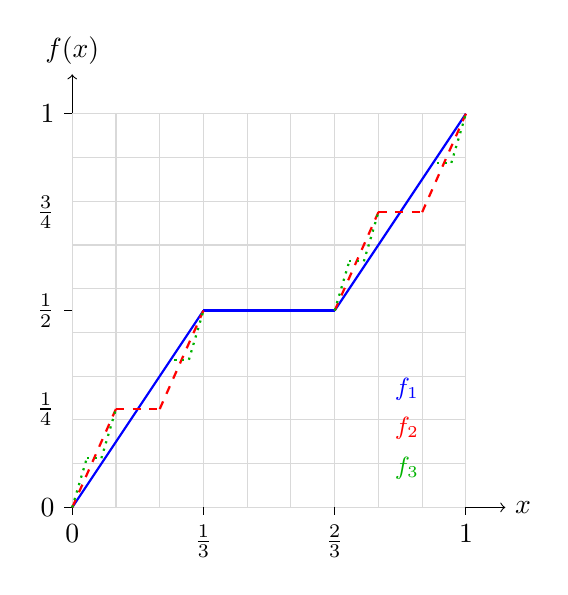
\begin{tikzpicture}[scale=5]
    % Axes
    \draw[->] (0,0) -- (1.1,0) node[right] {$x$};
    \draw[->] (0,0) -- (0,1.1) node[above] {$f(x)$};
    
    % Grid lines
    \draw[gray!30] (0,0) grid[step=1/9] (1,1);
    
    % Tick marks and labels on x-axis
    \foreach \x in {0, 1/3, 2/3, 1} {
        \draw (\x,0) -- (\x,-0.02);
    }
    \node[below] at (0,-0.02) {$0$};
    \node[below] at (1/3,-0.02) {$\frac{1}{3}$};
    \node[below] at (2/3,-0.02) {$\frac{2}{3}$};
    \node[below] at (1,-0.02) {$1$};
    
    % Tick marks and labels on y-axis
    \foreach \y in {0, 1/2, 1} {
        \draw (0,\y) -- (-0.02,\y);
    }
    \node[left] at (-0.02,0) {$0$};
    \node[left] at (-0.02,1/4) {$\frac{1}{4}$};
    \node[left] at (-0.02,1/2) {$\frac{1}{2}$};
    \node[left] at (-0.02,3/4) {$\frac{3}{4}$};
    \node[left] at (-0.02,1) {$1$};
    
    % Cantor function approximation (first few iterations)
    % Level 0: [0,1] -> [0,1]
    % Level 1: constant on (1/3, 2/3)
    \draw[thick, blue] (0,0) -- (1/3,1/2);
    \draw[thick, blue] (1/3,1/2) -- (2/3,1/2);
    \draw[thick, blue] (2/3,1/2) -- (1,1);
    
    % Level 2: constant on (1/9, 2/9) and (7/9, 8/9)
    \draw[thick, red, dashed] (0,0) -- (1/9,1/4);
    \draw[thick, red, dashed] (1/9,1/4) -- (2/9,1/4);
    \draw[thick, red, dashed] (2/9,1/4) -- (1/3,1/2);
    \draw[thick, red, dashed] (2/3,1/2) -- (7/9,3/4);
    \draw[thick, red, dashed] (7/9,3/4) -- (8/9,3/4);
    \draw[thick, red, dashed] (8/9,3/4) -- (1,1);
    
    % Level 3: even finer steps (showing the staircase nature)
    \draw[thick, green!70!black, dotted] (0,0) -- (1/27,1/8);
    \draw[thick, green!70!black, dotted] (1/27,1/8) -- (2/27,1/8);
    \draw[thick, green!70!black, dotted] (2/27,1/8) -- (1/9,1/4);
    \draw[thick, green!70!black, dotted] (7/27,3/8) -- (8/27,3/8);
    \draw[thick, green!70!black, dotted] (8/27,3/8) -- (1/3,1/2);
    
    % Additional fine structure
    \draw[thick, green!70!black, dotted] (2/3,1/2) -- (19/27,5/8);
    \draw[thick, green!70!black, dotted] (19/27,5/8) -- (20/27,5/8);
    \draw[thick, green!70!black, dotted] (20/27,5/8) -- (7/9,3/4);
    \draw[thick, green!70!black, dotted] (25/27,7/8) -- (26/27,7/8);
    \draw[thick, green!70!black, dotted] (26/27,7/8) -- (1,1);
    
    % % Endpoint dots
    % \fill[blue] (0,0) circle (0.8pt);
    % \fill[blue] (1/3,1/2) circle (0.8pt);
    % \fill[blue] (2/3,1/2) circle (0.8pt);
    % \fill[blue] (1,1) circle (0.8pt);
    
    % Legend
    \node[blue] at (0.85,0.3) {\small $f_1$};
    \node[red] at (0.85,0.2) {\small $f_2$};
    \node[green!70!black] at (0.85,0.1) {\small $f_3$};

    % Title
    % \node at (0.5,1.05) {\textbf{Cantor Function (Devil's Staircase)}};
\end{tikzpicture}
% \caption{The Cantor function showing its characteristic "devil's staircase" appearance. The function is constant on each removed interval from the Cantor set construction and increases only on the Cantor set itself.}
\label{fig:cantor_function}
\end{figure}

\begin{remark}
    The Cantor function has several remarkable properties:
    \begin{enumerate}
        \item It is continuous and non-decreasing on $[0,1]$.
        \item It maps $[0,1]$ onto $[0,1]$ surjectively.
        \item Its derivative is zero almost everywhere (on the complement of the Cantor set).
        \item It increases only on the Cantor set, which has measure zero.
        \item It is an example of a singular function: continuous but not absolutely continuous.
    \end{enumerate}
\end{remark}


% \chapter{Causal Inference}
% Rubin (1975\cite{rubin1975bayesian}) and Holland (1986\cite{holland1986statistics}) made up the aphorism\cite{ding2023causalinference}:
\begin{quote}
  \textit{``No causation without manipulation''}
\end{quote}
Not everybody agrees with this point of view.

In our lectuere, we'll define causal effects using the potential outcomes framework
(Neyman, 1923\cite{neyman1923experiment}; Rubin, 1974\cite{rubin1974estimating}).


\section{Potential Outcomes Framework}

In this framework, an experiment, or at least a thought experiment, 
has a treatment, and we are interested in its effect on an outcome 
or multiple outcomes. Sometimes, the treatment is also called an
intervention or a manipulation.

Firstly, we consider an experiment with $n$ units indexed by $i=1, 2, \cdots, n$.
We focus on a treatment with two levels:
\begin{gather*}
  d_i = \left\{\begin{matrix}
    0 & \text{control}\\
    1 & \text{treatment}
  \end{matrix} \right.
\end{gather*}

We seek to identify the causal effect of treatment $d_i$ on some outcome $y_i$.
For each $i$, the outcome od interest $y_i$ has two versions:
\begin{gather*}
  y_i = \left\{\begin{matrix}
    y_{0i} & d_i=0\\
    y_{1i} & d_i=1
  \end{matrix} \right.
\end{gather*}
This notation emphasizes that $y_{di}$ is the realization of the outcome $y_i$ that would materialize if unit $i$
received treatment $d_i = d$.

Neyman (1923\cite{neyman1923experiment}) first used this notation. It seems intuitive but has some hidden
assumptions. Rubin (1980\cite{rubin1980comment}) made the following clarifications on the hidden assumptions.
\begin{assumption}[No interference]\label{assumption:no_interference}
  \

  Unit $i$'s potential outcomes do not depend on other units' treatments. 
  This is sometimes called the no-interference assumption.
\end{assumption}
\begin{assumption}[Consistency]\label{assumption:consistency}
  \

  There are no other versions of the treatment. 
  Equivalently, we require that the treatment levels be well-defined, 
  or have no ambiguity at least for the outcome of interest. 
  This is sometimes called the consistency assumption.
\end{assumption}

The causal effect of the treatment on the $i$-th unit is then defined as:
\begin{gather*}
  \Delta_i = y_{1i} - y_{0i} 
\end{gather*}
These potential outcomes are constants at the level of unit $i$.

\begin{remark}[Problem of causal inference]
  \

  The fundamental problem in causal inference is that only one treatment can be assigned to a given individual, 
  and so only one of $y_{0i}$ and $y_{1i}$ can be observed. Thus $\Delta_i$ can never be observed.
\end{remark}

\begin{definition}[Stable Unit Treatment Value Assumption (SUTVA)]
\label{def:sutva}
  \

  Rubin (1980\cite{rubin1980comment}) called the Assumptions \ref{assumption:no_interference} and \ref{assumption:consistency} above together 
  the \textit{Stable Unit Treatment Value Assumption (SUTVA).}
\end{definition}
The observed outcome of unit $i$ is a function of the potential
outcomes and the treatment indicator, we can write:
\begin{gather*}
  y_i = d_i y_{1i} + (1 - d_i) y_{0i}
\end{gather*}
In principle, by virtue of being (discrete) RVs, both $d_i$ and $y_i$ each have a distribution function,
which, together with their possible realizations, defines various moments.
However, their unconditional probabilities and moments at the level of unit $i$ is not of interest.
Only the conditional probabilities of $y_i$ given $d_i$ is of interest.

\begin{remark}[Rubin (2005\cite{rubin2005causal})]
  \

  Under SUTVA, Rubin (2005) called the $n \times 2$ matrix of potential outcomes the Science Table:
  $$\begin{array}{ccc}
  \hline
  i & y_{1i}  & y_{0i}  \\
  \hline
  1 & y_{11}  & y_{01}  \\
  2 & y_{12}  & y_{02}  \\
  \vdots & \vdots & \vdots \\
  n & y_{1n}  & y_{0n} \\
  \hline
  \end{array}$$
  Due to the fundamental contributions of Neyman and Rubin to statistical causal inference, the potential outcomes framework is sometimes referred to as the Neyman Model, 
  the Neyman-Rubin Model, or the Rubin Causal Model.
  Causal effects are functions of the Science Table. Inferring individual causal effects
  $$\tau_i = y_{1i}  - y_{0i} , \quad (i=1,\ldots,n)$$
  is fundamentally challenging because we can only observe either $y_{1i} $ or $y_{0i}$,
  for each unit $i$, that is, we can observe only half of the Science Table.
\end{remark}

SUTVA(\ref{def:sutva}) ensures that the individual treatment effect is well defined.

Now, although $\Delta_i$ itself is unobservable, we can (perhaps remarkably) 
use randomized experiments to learn certain properties of it. The expectations
$\mathbb{E}[y_{0i}]$ and $\mathbb{E}[y_{1i}]$ denote the average potential outcomes across unit $i$ in population.

In particular, large randomized experiments let us recover the \textbf{Average
Treatment Effect (ATE)}:
\begin{gather*}
  \text{ATE} = \mathbb{E}[y_{1i} - y_{0i}] = \mathbb{E}[y_{1i}] - \mathbb{E}[y_{0i}]
\end{gather*}

For a population, we can define the treatment conditional expectations:
\[\mathbb{E}[y_i | d_i=1], \mathbb{E}[y_{0i} | d_i=1 ], \mathbb{E}[y_{1i} | d_i=1 ] = \mathbb{E}[y_i | d_i=1]\]
that denote the averages of the outcome $y_i$.

Analogously, we can define the control conditional expectations:
\[\mathbb{E}[y_i | d_i=0], \mathbb{E}[y_{0i} | d_i=0 ] = \mathbb{E}[y_i | d_i=0], \mathbb{E}[y_{1i} | d_i=0 ]\]
for the non-treated subpopulation.

Similar to ATE, we candefine the Average Treatment Effect for the Treatment-Group (ATT) and the Average
Treatment Effect for the Control-Group (ATC) as distinct objects:
\begin{align*}
  \text{ATT} &= \mathbb{E}[y_{1i}- y_{0i} | d_i=1]\\
  \text{ATC} &= \mathbb{E}[y_{1i}- y_{0i} | d_i=0]
\end{align*}
\[\mathbb{E}[z] = \mathbb{E}[z|d=1] \mathbb{P}[d=1] + \mathbb{E}[z|d=0] \mathbb{P}[d=0] = \mathbb{E}[\mathbb{E}[z|d]].\]

\subsection{Identification of Causal Effects}

Now, suppose we observe treatments and outcomes over a random sample $n$ from the overall population, $\{d_i, y_i\}_{i=1}^n = \{d_i, y_{d_{i}i}\}_{i=1}^n$, 
as either $y_I = y_{0i} $, or $y_i = y_{1i}$. 

Let $n_{w} = \vert \{ i: d_i = w \} \vert $ be the size of sets of units in our
sample who received and did not receive treatment, respectively.
This means that: while we observe a sample of size $n$ of $d_i$ and $y_i$ from the overall population,
we are observing a sample of size $n_0$ of realizations of $y_{0i}$ from the non-treated subpopulation 
and a sample of size $n_1$ of realizations of $y_{1i}$ from the treated subpopulation.

$N = \{i=1,2,\cdots, n\}$, $N_1 = \{i \in N: d_i = 1\} \leftarrow n_1 = \vert N_1 \vert $, $N_0 = \{i: d_i = 0\} \leftarrow n_0 = \vert N_0 \vert $.

Based on this data, we can use the analogy principle to consistently estimate 
the first term in the ATT formula and the second term in the ATC formula:
\begin{align*}
  \frac{1}{n_1} \sum_{i \in N_1} y_i &= \frac{1}{n_1} \sum_{i \in N_1} y_{1i} \overset{p}{\rightarrow} \mathbb{E}[y_{1i} | d_i=1] = \mathbb{E}[y_i | d_i=1]\\
  \frac{1}{n_0} \sum_{i \in N_0} y_i &= \frac{1}{n_0} \sum_{i \in N_0} y_{0i} \overset{p}{\rightarrow} \mathbb{E}[y_{0i} | d_i=0] = \mathbb{E}[y_i | d_i=0]
\end{align*}
Without further assumptions, we cannot identify the remaining terms. Firstly, we cannot observe $\mathbb{E}[y_{0i} | d_i=1]$ and $\mathbb{E}[y_{1i} | d_i=0 ]$
because we do not observe $y_{0i}$ for treated units, and we do not observe $y_{1i}$ for non-treated units.
Secondly, we can not observe $\mathbb{E}[y_{1i}]$ and $\mathbb{E}[y_{0i}]$ because both $N_1$ and $N_0$ are random samples from the overall population.
As a result, the ATE is in general not identified from our data!

We can define the  the difference-in-means estimator as:
\[\hat{\tau}_{DM} = \frac{1}{n_1} \sum_{i \in N_1} y_i - \frac{1}{n_0} \sum_{i \in N_0} y_i \overset{p}{\rightarrow} \mathbb{E}[y_{1i} | d_i = 1] - \mathbb{E}[y_{0i} | d_i = 0] = \text{ATE} = \text{ATT} = \text{ATC}.\]


We define the difference of treated and non-treated as: \textit{Naive Difference}.
\begin{align*}
  \text{ND} &= \mathbb{E}[y_{1i} | d_i = 1] - \mathbb{E}[y_{0i} | d_i = 0]\\
  &= \mathbb{E}[y_{1i} | d_i = 1] - \mathbb{E}[y_{0i} | d_i = 1] + \mathbb{E}[y_{0i} | d_i =1] - \mathbb{E}[y_{0i} | d_i = 0] \\
  &= ATT + \mathbb{E}[y_{0i} | d_i = 1] - \mathbb{E}[y_{0i} | d_i = 0]
\end{align*}

For LRM, $y_i = \beta_0 + \beta_1 d_i + u_i$,
\begin{align*}
  \text{ND} &= \mathbb{E}[y_i | d_i = 1] - \mathbb{E}[y_i | d_i = 0]\\
  &= \mathbb{E}[\beta_0 + \beta_1 + u_i | d_i = 1] - \mathbb{E}[\beta_0 + u_i | d_i = 0]\\
  &= \beta_1 + \mathbb{E}[u_i | d_i = 1] - \mathbb{E}[u_i | d_i = 0]  
\end{align*}



\[
\{Y_d\} \perp\!\!\!\perp D \mid X \implies \{Y_d\} \perp\!\!\!\perp D \mid \pi(X), \quad D \perp\!\!\!\perp X \mid \pi(X)
\]
% \chapter{Panel Data Analysis}
% Economists traditionally use the term \textbf{panel data} to refer to data structures consisting of observa-
tions on individuals for multiple time periods. 
There are several distinct advantages of panel data relative to cross-section data:
\begin{enumerate}
  \item Possibility of controlling for unobserved time-invariant endogeneity without the use of instrumental variables
  \item Possibility of allowing for broader forms of heterogeneity
  \item Modeling dynamic relationships and effects
\end{enumerate} 

It's typical to index observations by both the individual $i$ and the time period, $t$,
thus $y_{it} $ denotes a variable for indivual $i$ in time $t$, where $n=1, \cdots, N$, $t=1, \cdots, T.$

\begin{definition}[Balanced and Unbalanced Panel Data\cite{hansen2022econometrics}]
  \

  When observations are available on all individuals for the same time periods we say that the panel is \textbf{balanced}. 
  In this case there are an equal number $T$ of observations for each individual and the total number of observations is $n = NT$.

  When different time periods are available for the individuals in the sample we say that the panel is \textbf{unbalanced}. 
  This is the most common type of panel data set. 
  It does not pose a problem for applications but does make the notation cumbersome and also complicates computer programming.
\end{definition}

\section{Incidental Parameters Problem}

\subsection{Pooled OLS Estimation}\label{sec:POLS}

Suppose we are estimating the following panel data regression:
\begin{align*}
  y_{it} &= \alpha +x_{it}^{\prime} \beta +u_{it}, \quad \mathbb{E}[u_{it} x_{it}] = 0, \quad \mathbb{V}[u_{it} | x_{it}] = \sigma^2
\end{align*}

Omitting the distinction between intercept and slope, we can write the model as:
\begin{gather*}
  y_{it} = \tilde{x}_{it}^{\prime} \tilde{\beta} + u_{it} \\
  \tilde{x}_{it} = \begin{bmatrix}
    1 \\
    x_{it}
  \end{bmatrix}, \quad
  \tilde{\beta} = \begin{bmatrix}
    \alpha \\
    \beta
  \end{bmatrix}
\end{gather*}
where $i=1:n$, $T=1:t$.

Or, we can write the model as: 
\[ 
\underset{T\times 1}{y_i} = \underset{T \times K}{\tilde{X}_i} \underset{K \times 1}{\tilde{\beta}} + \underset{T \times 1}{u_i}
\]
Using OLS method to estimate $\tilde{\beta}$, we have:
\[
\underset{\tilde{\beta}}{\min} \sum_i \sum_t u_{it}^2 = \underset{\tilde{\beta}}{\min} \sum_i u_i^{\prime} u_i = \underset{\tilde{\beta}}{\min} (y_i - \tilde{X}_i \tilde{\beta})^{\prime} (y_i - \tilde{X}_i \tilde{\beta})
\]
The FOC of this equation is:
\begin{align*}
  \sum_i -\tilde{X}_i^{\prime} (y_i - \tilde{X}_i \tilde{\beta}) &= 0 \\
  \left(\sum_i \tilde{X}_i^{\prime} \tilde{X}_i \right) \tilde{\beta} &= \sum_i \tilde{X}_i^{\prime} y_i \\
  \hat{\tilde{\beta}}_{POLS} &= \left(\sum_i \tilde{X}_i^{\prime} \tilde{X}_i \right)^{-1} \sum_i \tilde{X}_i^{\prime} y_i \\
  &= \left(\sum_i \sum_t \tilde{x}_{it} \tilde{x}_{it}^{\prime} \right)^{-1} \left( \sum_i \sum_t \tilde{x}_{it} y_{it} \right) \\
  &= \tilde{\beta} + \left(\frac{1}{n} \sum_i \sum_t \tilde{x}_{it} \tilde{x}_{it}^{\prime} \right)^{-1} \left( \sum_i \sum_t \tilde{x}_{it} u_{it} \right) \\
  & \overset{p}{\rightarrow} \tilde{\beta} + \mathbb{E}\left[\sum_t \tilde{x}_{it} \tilde{x}_{it}^{\prime} \right] \mathbb{E}\left[\sum_t \tilde{x}_{it} u_{it} \right] \\
  &= \tilde{\beta}
\end{align*}
Hence $\hat{\beta}_{OLS}$ is consistent provided that $x_{it}$ and $u_{it}$ are contemperaneously uncorrelated,
as $\mathbb{E}[x_{it} u_{it}] = 0, \forall t.$
The regressors are allowed to be correlated with the past, and future $u_{it}$.
This occurs when there's feedback loop by which $y_{i,t-1}$ affects $x_{it}$.

In this proof, we show that either $N \to \infty $ or $T \to  \infty $ is sufficient for consistency of $\hat{\beta}_{POLS}$.
However, most panel data applications have a large $n$ and small $T$ dimension, so standrad panel data
features $T$ fixed and $n \to \infty $.

\subsection{Asymptotic Normality}

From the analysis of consistency, we know that:
\[ 
\hat{\tilde{\beta}}_{POLS}  = \left(\sum_i \tilde{X}_i^{\prime} \tilde{X}_i \right)^{-1} \sum_i \tilde{X}_i^{\prime} y_i
\]
Hence:
\begin{align*}
    \sqrt{n} (\hat{\tilde{\beta}}_{POLS}  - \tilde{\beta}) &= \left(\frac{1}{n} \sum_i \tilde{X}_i^{\prime} \tilde{X}_i \right)^{-1} \left(\frac{1}{\sqrt{n} } \sum_i \tilde{X}_i^{\prime} u_i \right) \\
    & \overset{p}{\rightarrow}\mathbb{E}[\tilde{X}_i^{\prime} \tilde{X}_i]^{-1} \overset{d}{\rightarrow} \mathcal{N}\left(0, \mathbb{E}\left[\left(\tilde{X}_i^{\prime} u_i\right) \left(\tilde{X}_i^{\prime} u_i\right)^{\prime} \right] \right)\\
    & \overset{d}{\rightarrow} \mathcal{N} \left(0, \mathbb{E}\left[\tilde{X}_i^{\prime} \tilde{X}_i \right]^{-1} \mathbb{E}\left[\tilde{X}_i^{\prime} u_i u_i^{\prime} \tilde{X}_i \right] \mathbb{E}\left[\tilde{X}_i^{\prime} \tilde{X}_i \right] \right)
\end{align*}


The above model is homogeneous, which is unattractive, as the data generating process would 
differ across $i$, with some units having a higher level of the outcome variable $y_{it} $
than others, regardless of covariates $x_{it}$(with a higher intercept $\alpha$) or a stronger effect
of some covariates $x_{it, k} $ on $y_{it}$ than others.

At the other extreme, we assume the fully heterogenous estimation:
\[y_{it} = \alpha_i + x_{it}^{\prime} \beta + u_{it}, \quad \mathbb{E}[u_{it} x_{it}] = 0, \quad \mathbb{V}[u_{it} | x_{it}] = \sigma_i^2. \]

Under $T=1$, we run $y_i = \beta_0 + x_i^{\prime} \beta + v_i$, 
where $v_i = u_i + \underset{\tilde{\alpha}_i}{\underbrace{\alpha_i - \beta_0}}$
and $\mathbb{E}[v_i] = 0$.

Under $T>1$, we run:
\begin{align*}
    y_i &= x_i^{\prime} \beta  + \sum_{j=1}^{n} \alpha_j \mathbf{1}\{i=j\} + u_{it} \\
    &= \tilde{x}_{it}^{\prime} \tilde{\beta} + u_{it} \\
    \tilde{x}_{it} &= \begin{bmatrix}
      x_{it} \\
      \mathbf{1}\{i=1\} \\
      \mathbf{1}\{i=2\} \\
      \vdots \\
      \mathbf{1}\{i=n\}
    \end{bmatrix}, \quad
    \tilde{\beta} = \begin{bmatrix}
      \beta \\
      \alpha_1 \\
      \alpha_2 \\
      \vdots \\
      \alpha_n
    \end{bmatrix}
\end{align*}

In a similar way, we can write the regression as
\[y_{i}  = \tilde{X}_i \tilde{\beta}_i + u_i \]
with $\tilde{\beta}_i$ is specific for each $i$.
We have $n$ separate time series regressions, one for each unit $i$. 

Following the same analyzing process, we can get:
\[
\hat{\tilde{\beta}}_{i,OLS} = \Bigl( \sum_i \tilde{X}_i^{\prime} \tilde{X}_i \Bigr) \sum_i \tilde{X}_i^{\prime} y_i = \Bigl( \sum_t \tilde{x}_{it} \tilde{x}_{it}^{\prime} \Bigr)^{-1} \Bigl( \sum_t \tilde{x}_{it} y_{it} \Bigr),
\]
which obviously shows that $\hat{\tilde{\beta}}$ is consistent $\operatorname{\iff}$ $T \rightarrow\infty $.

\subsection{One-way error component model}\label{sec:one-way error component model}
With the fully homogeneous specification unattractive and the fully heterogeneous specifi-
cation infeasible, researchers usually go for a compromise and let intercepts (and error term
variances) be unit-specific.

\begin{definition}[One-way error component model]
  \begin{equation}
    y_{it}  = \alpha_i + x_{it}^{\prime} + u_{it}, \quad \mathbb{E}[u_{it} x_{it}] = 0, \quad \mathbb{V}[u_{it} | x_{it}] = \sigma^2, \label{eq: basic model}
  \end{equation}
where $\alpha_i$ is an individual-specific effect, and $u_{it}$ are idiosyncratic(i.i.d.) errors.
\end{definition}

In any case, the equation above makes clear that $\alpha_i $ contains all factors that affect $y_{it}$, that are
not included in $x_{it}$ and that are fixed over time (the time-varying factors are in $u_{it}$).

Suppose hte model is correctly specified, and we have a cross-sectional detaset available, i.e. $T=1$.
Then, we would estimate:
\[y_{it} = \beta_0 + x_{it}^{\prime} + v_i, \text{ for} t=1,\]
where $v_i = \alpha_i + u_{it} -\beta_0.$

If the unobserved heterogeneity $\alpha_i$ is correlated with the covariate $x_{it} $,
our standard OLS estimator is biased and inconsistent.

If we have a panel dataset, i.e. $T>1$, we can write the above model into a regression of $k+n$ regressors:
\[
y_{it} = x_{it}^{\prime} \beta + \sum_{j=1}^{n}\mathbf{1}\{i=j\} \alpha_j + u_{it} = x_{it}^{*^{\prime}} \beta^* + u_{it},
\]
where $x_{it}^* = \Bigl( x_{it}^{\prime}, \mathbf{1}\{i=1\}, \cdots, \mathbf{1}\{i=n\} \Bigr)^{\prime} $,
and $\beta^* = \Bigl( \beta^{\prime}, \alpha_1, \cdots, \alpha_n \Bigr)^{\prime}.$

This leads to the pooled OLS estimator for $\beta^*$:
\[
\hat{\beta}^* = \Bigl( \sum_i \sum_t x_{it}^* x_{it}^{*^{\prime}} \Bigr) \sum_i \sum_t x_{it}^* y_{it}. 
\]

However, the estimator suffers from the so-called \textbf{IPP problem}, 
as the number of parameters increase with $n \rightarrow\infty $, 
the limit of $\frac{1}{n} \sum_i x_{it}^* x_{it}^{*^{\prime}}$ is not well-defined
and as a result, we can't establish consistency of $\hat{\beta}_{OLS}.$
% \section{Random Effects}

As with pooled OLS, a random effects analysis puts $\alpha_i$ into the error term.
In fact, random effects analysis imposes more assumptions than those needed for pooled OLS:
\textbf{strict exogeneity} in addition to orthogonality between $\alpha_i$ and $x_{it}$. 

\subsection{Basic Assumptions and POLS}

Stating the assumption in terms of conditional means, we have:
\begin{assumption}[Random Effect]\label{assumption:RE}
    \

    \begin{enumerate}
        \item[(a)] $\mathbb{E}[u_{it} | X_i, \alpha_i] = 0, \forall t.$
        \item[(b)] $\mathbb{E}[\alpha_i | X_i] = \mathbb{E}[\alpha_i] = 0.$
    \end{enumerate}
    where $X_i = (x_{i1}, \cdots, x_{iT})$.
\end{assumption}
Assumption \ref{assumption:RE}(a) is the strict exogeneity condition and Assumption \ref{assumption:RE}(b) is is how we will state the orthogonality.

\begin{remark}[Why Strict Ecogeneity?\cite{wooldridge2010econometric}]
    \

    Why do we maintain Assumption \ref{assumption:RE}(a) when it is more restrictive than needed for
    a pooled OLS analysis? Because the random e¤ects approach exploits the serial correlation in
    the composite error, $v_{it} = \alpha_i + u_{it}$, in a generalized least squares (GLS) framework. In
    order to ensure that feasible GLS is consistent, we need some form of strict exoge-
    neity between the explanatory variables and the composite error.

    Under this assumption, we can write:
    \begin{align*}
        & y_{it} = x_{it}^{\prime} \beta + v_{it} \\
        & \mathbb{E}[v_{it} | X_i] = 0, t=1, \cdots, T
    \end{align*}
    The conditions shows that our model satisfies the GLS assumption, which confirms that
    we can apply GLS methods that account for the particular error structure $v_{it} = \alpha_i + u_{it}.$
\end{remark}


By defining $v_{it} = u_{it} + \alpha_i - \beta_0$, we can transform the random effect model to the following:
\begin{align*}
    y_{it} &= \alpha_i + x_{it}^{\prime} \beta + u_{it} \\
    &= \underset{\tilde{x}_{it}^{\prime}}{\underbrace{\beta_0 + x_{it}^{\prime}\beta}} + \underset{\equiv v_{it}}{\underbrace{u_{it} + \alpha_i - \beta_0}}
\end{align*}
Defining again $\tilde{x}_{it} = (1, x_{it}^{\prime})^{\prime}$, $\tilde{\beta} = (\beta_0, \beta^{\prime})^{\prime}$, we can rewrite the model as:
\begin{align*}
    y_{it} &= \tilde{x}_{it}^{\prime} \beta + v_{it} \Leftrightarrow y_i = \tilde{X}_i^{\prime} \tilde{\beta} + v_i \\
    \rightarrow \hat{\tilde{\beta}} &= \left(\sum_i \tilde{X}_i^{\prime} \tilde{X}_i \right)^{-1} \sum_i \tilde{X}_i^{\prime} y_i
\end{align*}

With this intercept $beta_0$, $\mathbb{E}[v_i] = 0$ is guaranteed to hold.
Define $\tilde{\alpha}_i = \alpha_i - \beta_0$ as the mean-zero unit-specific heterogenety so that $v_i = u_i + \tilde{\alpha}_i.$


\begin{note}[POLS]
    \

    Homogenous spec: $y_{it} = \alpha  + x_{it}^{\prime} \beta + u_{it} = \tilde{x}_{it}^{\prime} \tilde{\beta} + v_{it}.$
    $\hat{\tilde{\beta}}$ is consistent if $\mathbb{E}[v_{it} x_{it}]=0, \forall t.$
\end{note}
Using pooled OLS to estimate $\hat{\tilde{\beta}}$,
\begin{align*}
    \hat{\tilde{\beta}}_{RE-OLS/POLS} &= \left(\frac{1}{n} \sum_i \tilde{X}_i^{\prime} \tilde{X}_i \right)^{-1} \frac{1}{n} \sum_i \tilde{X}_i^{\prime} y_i \\
    &= \tilde{\beta} + \left(\frac{1}{n} \sum_i \tilde{X}_i^{\prime} \tilde{X}_i \right)^{-1} \frac{1}{n} \sum_i \tilde{X}_i^{\prime} v_i \\
    &\overset{p}{\rightarrow} \tilde{\beta} + \mathbb{E}[\tilde{X}_i^{\prime} \tilde{X}_i]^{-1} \mathbb{E}[\tilde{X}_i^{\prime} v_i] \\
    \text{where} \quad \mathbb{E}[\tilde{X}_i^{\prime} v_i] &= \mathbb{E}\left[\sum_t \tilde{x}_{it}^{\prime} v_{it} \right] \\
    &= \sum_t \mathbb{E}\left[\tilde{x}_{it}^{\prime} v_{it}  \right] \\
    &= \sum_t \mathbb{E}\left[\tilde{x}_{it}(u_{it} + \alpha_i - \beta_0)\right]
\end{align*}
Here, the error term $v_i$ is not equal to the original error term $u_{it}$.
\begin{note}
    \

    Under the random effect, you have to use the heteroskedasticity-robust methods.
    Because even if we assume $u_{it}$ to be homoskedastic, $v_{it}$ is not,
    as it includes also the unit-specific heterogeneity $\alpha_i$.
\end{note}

\subsection{From POLS to GLS}

So, to obtain consistency, we need to assume that:
\begin{itemize}
    \item $\mathbb{E}[u_{it} | \tilde{x}_{it}, \tilde{\alpha}_i] = 0, \forall t$.
    \item $\mathbb{E}[\tilde{\alpha_i} | \tilde{x}_{it}] = 0, \forall t$.
\end{itemize}
And, we are also obliged to use HAC-robust standard error because:
\[\Omega \equiv \mathbb{E}[v_i v_i^{\prime} | \tilde{X}_i] = \mathbb{E}[(\alpha_i \mathbf{1}_i + u_i)(\tilde{\alpha}_i \mathbf{1}_i + u_i)^{\prime} | \tilde{X}_i] = \mathbb{E}[\tilde{\alpha}_i^2 \mathbf{1}_i \mathbf{1}_i^{\prime} | \tilde{X}_i] + \mathbb{E}[u_i u_i'| \tilde{X}_i] \]
is not diagonal.

\begin{assumption}[Random Effect]\label{assumption:RE2}
    \

    $\rank \mathbb{E}\left[X_i^{\prime} \Omega^{-1} X_i \right] = K$
\end{assumption}
We know that both GLS and feasible GLS estimator would be consistent under Asusmption \ref{assumption:RE} and \ref{assumption:RE2}.
A general FGLS analysis, using an unrestricted variance estimator $\Omega$,
is consistent and asymptotically normal as $N \to \infty.$

But, we won't exploit the unobserved effects structure $v_{it}.$
A standard random e¤ects analysis adds assumptions on the idiosyncratic errors that
give $\Omega$ a special form. The first assumption is that the idiosyncratic errors
$u_{it}$ have a constant unconditional variance across $t$:
\begin{assumption}[RE-Homoskedasticity]\label{assumption:RE-homoskedasticity}
    \

    $\mathbb{E}[u_{it}^2] = \sigma_u^2, \forall t$
\end{assumption}
The second assumption is that the idiosyncratic errors are serially uncorrelated:
\begin{assumption}[RE-Serial Uncorrelated]\label{assumption:RE-serial_uncorrelated}
    \

    $\mathbb{E}[u_{it} u_{is}] = 0, \forall t \neq s$
\end{assumption}
Under these two assumptions, we can derive the variances and covariances of the
elements of $v_i$.
Given the error structure the natural estimator for $\beta$ is GLS. The GLS eimator for $\beta$ is:
\begin{gather*}
    \hat{\tilde{\beta}}_{RE-GLS} = \left( \sum_i \tilde{X}_i^{\prime} \Omega^{-1} \tilde{X}_i \right)^{-1} \sum_i \tilde{X}_i^{\prime} \Omega^{-1} y_i
\end{gather*}
where $\Omega ^{-\frac{1}{2}} y_i = \Omega ^{-\frac{1}{2}} \tilde{X}_i^{\prime} \tilde{\beta} + \Omega^{-\frac{1}{2}}v_i.$
\begin{align*}
    \Omega &= \mathbb{E}[v_i v_i^{\prime} | \tilde{X}_i] = \mathbb{E}\left[ \begin{bmatrix}
        v_{i1} \\
        v_{i2} \\
        \vdots \\
        v_{iT}
    \end{bmatrix} \begin{bmatrix}
        v_{i1} & v_{i2} & \cdots & v_{iT}
    \end{bmatrix} | \tilde{X}_i \right]\\
    &= \mathbb{E}\begin{bmatrix}
        \mathbb{E}[v_{i1}^2 | \tilde{X}_i] & \mathbb{E}[v_{i1}v_{i2} | \tilde{X}_i] & \cdots & \mathbb{E}[v_{i1}v_{iT} | \tilde{X}_i] \\
        \mathbb{E}[v_{i2}v_{i1} | \tilde{X}_i] & \mathbb{E}[v_{i2}^2 | \tilde{X}_i] & \cdots & \mathbb{E}[v_{i2}v_{iT} | \tilde{X}_i] \\
        \vdots & \vdots & \ddots & \vdots \\
        \mathbb{E}[v_{iT}v_{i1} | \tilde{X}_i] & \mathbb{E}[v_{iT}v_{i2} | \tilde{X}_i] & \cdots & \mathbb{E}[v_{iT}^2 | \tilde{X}_i]
    \end{bmatrix} \\
    &= \begin{bmatrix}
        \mathbb{E}\left[\alpha_i^2 | \tilde{X}_i \right] + \mathbb{E}[u_{i1}^2 | \tilde{X}_i] & \mathbb{E}\left[\alpha_i^2 | \tilde{X}_i \right] + \mathbb{E}[u_{i1}u_{i2} | \tilde{X}_i] & \cdots & \mathbb{E}\left[\alpha_i^2 | \tilde{X}_i \right] + \mathbb{E}[u_{i1}u_{iT} | \tilde{X}_i] \\
        \mathbb{E}\left[\alpha_i^2 | \tilde{X}_i \right] + \mathbb{E}[u_{i2}u_{i1} | \tilde{X}_i] & \mathbb{E}\left[\alpha_i^2 | \tilde{X}_i \right] + \mathbb{E}[u_{i2}^2 | \tilde{X}_i] & \cdots & \mathbb{E}\left[\alpha_i^2 | \tilde{X}_i \right] + \mathbb{E}[u_{i2}u_{iT} | \tilde{X}_i] \\
        \vdots & \vdots & \ddots & \vdots \\
        \mathbb{E}\left[\alpha_i^2 | \tilde{X}_i \right] + \mathbb{E}[u_{iT}u_{i1} | \tilde{X}_i] & \mathbb{E}\left[\alpha_i^2 | \tilde{X}_i \right] + \mathbb{E}[u_{iT}u_{i2} | \tilde{X}_i] & \cdots & \mathbb{E}\left[\alpha_i^2 | \tilde{X}_i \right] + \mathbb{E}[u_{iT}^2 | \tilde{X}_i]
    \end{bmatrix}\\
    &= \begin{bmatrix}
        \sigma_u^2 + \sigma_{\alpha}^2 & \sigma_{\alpha}^2 & \cdots & \sigma_{\alpha}^2 \\
        \sigma_{\alpha}^2 & \sigma_u^2 + \sigma_{\alpha}^2 & \cdots & \sigma_{\alpha}^2 \\
        \vdots & \vdots & \ddots & \vdots \\
        \sigma_{\alpha}^2 & \sigma_{\alpha}^2 & \cdots & \sigma_u^2 + \sigma_{\alpha}^2
    \end{bmatrix} \\
    &= \sigma_{\alpha}^2 \mathbf{1}_i \mathbf{1}_i^{\prime} + \sigma_u^2 I \\
    \text{beacuse } &\mathbb{V}[\tilde{\alpha}_i|\tilde{X}_i] = \sigma_{\alpha_i}^2 = \sigma_{\alpha}^2 \\
    &\mathbb{V}[u_{it} | \tilde{X}_i] = \sigma_u^2, \forall i.
\end{align*}
where $I$ is an identity matrix of dimention $T_i$.
Under the assumption $\mathbb{E}[u_{it} x_{is}] = 0$, we now describe some statistical properties of $\hat{\tilde{\beta}}_{RE-GLS}.$

\subsubsection{RE Consistency}
\begin{align*}
    \hat{\tilde{\beta}}_{RE-GLS} - \tilde{\beta} &= \Bigl( \sum_i \tilde{X}_i^{\prime} \Omega^{-1} \tilde{X}_i \Bigr)^{-1} \Bigl( \sum_i \tilde{X}_i^{\prime} \Omega^{-1} v_i \Bigr) \\
    & \rightarrow \mathbb{E}\Bigl[ \sum_i \tilde{X}_i^{\prime} \Omega^{-1} \tilde{X}_i \Bigr] \mathbb{E}\Bigl[ \sum_i \tilde{X}_i^{\prime} \Omega^{-1} v_i \Bigr] \\
    \text{where } \mathbb{E}\Bigl[ \sum_i \tilde{X}_i^{\prime} \Omega^{-1} v_i \Bigr] &= \sum_i \mathbb{E}\Bigl[ \tilde{X}_i^{\prime} \Omega^{-1} v_i \Bigr] \\
    &= \sum_i \tilde{X}_i^{\prime} \Omega^{-1} \mathbb{E}[v_i | \tilde{X}_i] \\
    &= \sum_i \tilde{X}_i^{\prime} \Omega^{-1} \mathbb{E}[u_i + \tilde{\alpha}_i | \tilde{X}_i] \\
    &=0
\end{align*}
Thus, $\hat{\tilde{\beta}}_{RE-GLS} $ is conditionally unbiased for $\tilde{\beta}$.
The conditional variance of $\hat{\tilde{\beta}}_{RE-GLS}$ is:
\begin{align*}
    \mathbb{V}\Bigl[\hat{\tilde{\beta}}_{RE-GLS}\Bigr] = \Bigl( \sum_i \tilde{X}_i^{\prime} \Omega^{-1} \tilde{X}_i \Bigr)^{-1} \sigma_{u}^2
\end{align*}

\subsubsection{RE Asymptotic Distribution}
The asymptotic variance of $\hat{\tilde{\beta}}_{RE-GLS}$ is:
\begin{align*}
    &\sqrt{n} \left( \hat{\tilde{\beta}}_{RE-GLS} - \tilde{\beta} \right) \overset{d}{\rightarrow} \mathcal{N}\left(0, V \right) \\
    \text{where } V_{GLS}  &= \mathbb{E}\left[\tilde{X}_i^{\prime} \Omega^{-1} \tilde{X}_i \right]^{-1} \mathbb{E}\left[\tilde{X}_i^{\prime} \Omega^{-1} v_i v_i^{\prime} \Omega^{-1} \tilde{X}_i \right] \mathbb{E}\left[\tilde{X}_i^{\prime} \Omega^{-1} \tilde{X}_i \right] \\
    &= \mathbb{E}\left[\tilde{X}_i^{\prime} \Omega^{-1} \tilde{X}_i \right]^{-1} \underset{\equiv \Omega}{\underbrace{\mathbb{E}[v_i v_i^{\prime} | \tilde{X}_i]}}
\end{align*}
Because we do not know $\Omega$, the RE-GLS estimator is infeasible. 

If indeed we have:
\begin{align*}
    \Omega &= \mathbb{E}[v_i v_i^{\prime}  | \tilde{X}_i] \\
    &= \mathbb{E}[(\alpha_i \mathbf{1}_i + u_i)(\alpha_i \mathbf{1}_i  + u_i)^{\prime}  | \tilde{X}_i] \\
    &= \mathbb{E}[\alpha_i^2] \mathbf{1}_i \mathbf{1}_i^{\prime} + \mathbb{E}[u_i u_i^{\prime} | \tilde{X}_i]
\end{align*}
which implies homoskedasticity.

A feasible version replaces $\Omega$ with an estimator $\hat{\Omega}_i$.
Assuming homoskedasticity of the original errors:
\begin{align*}
    \mathbb{E}[u_i u_i^{\prime}  | \tilde{X}_i, \tilde{\alpha}_i] &= \sigma_u^2 I_T \\
    \mathbb{E}[\tilde{\alpha}_i^2 | \tilde{x}_i] &= \sigma_{\alpha}^2
\end{align*}
We obtain: $\hat{\Omega} = \hat{\sigma}_{\alpha}^2 \mathbf{1}_i \mathbf{1}_i^{\prime} + \hat{\sigma}_u^2 I_T$, 
a $T \times T$ matrix that we assume to be positive definite.
In a panel data context, the FGLS estimator that uses this variance matrix is what is known as the \textbf{random effects estimator}.

Hence, the motivation for using GLS is different than under a cross-sectional regression with heteroskedasticity.
We use GLS because of the autocorrelation in $v_{it}$ induced by the presence of time variant $\alpha_i$.

\subsection{Comparing POLS and GLS}

Now, let's compare the $\hat{\beta}_{RE-GLS}$ with the pooled estimator $\hat{\beta}_{POLS}$.

Under the assumptions of the random effects model, POLS estimator is also unbiased for $\beta$ and has conditional variance:
\begin{gather*}
    V_{POLS} = \Bigl(\sum_{i} X_i^{\prime} X_i \Bigr)^{-1} \Bigl( X_i^{\prime} \Omega_i X_i \Bigr)^{-1} \Bigl( X_i^{\prime} X_i \Bigr)^{-1} 
\end{gather*}
Using the algebra of the Gauss-Markov Theorem we deduce that:
\[V_{RE-GLS} \leq V_{POLS} \]
and thus the random effects estimator $\hat{\beta}_{RE-GLS}$ is more efficient than $\hat{\beta}_{POLS} $ under the strict exogeneity assumption \ref{assumption:RE}.
The two variance matrices are identical when there is no individual-specific effect $\sigma_{\alpha}^2 = 0$ for then $V_{RE-GLS} = V_{POLS} = \left(X^{\prime} X\right)^{-1} \sigma_u^2.$

Under the asusmption that the random effects model is a useful approximation but not literally true, 
we may use the cluster-robust covariance matrix estimator such as:
\begin{gather*}
    \hat{V}_{RE-GLS} = \Bigl(\sum_{i} X_i^{\prime} \Omega_i X_i\Bigr)^{-1} \Bigl( \sum_{i} X_i^{\prime} \Omega_i \hat{v}_i \hat{v}_i^{\prime} \Omega_i^{\prime} X_i \Bigr)^{-1} \Bigl( \sum_{i} X_i^{\prime} \Omega_i X_i \Bigr)^{-1} 
\end{gather*}
where $\hat{v}_i = y_i - X_i \hat{\beta}_{RE-GLS}$, This may be re-scaled by a degree of freedom adjustment if desired.

\section{Fixed Effects}
In the econometrics literature if the stochastic structure of $\alpha_i$ is treated as unknown
and possibly correlated with $x_{it}$, then $\alpha_i$ is called a \textbf{fixed effect}.

Correlation between $\alpha_i$ and $x_{it}$ will cause both pooled and random effect estimators ro be biased.

We transform equation to get rid of $\alpha_i$: $y_{it} = \alpha_i + x_{it}^{\prime} \beta + u_{it}.$
This is due to the classic problems of omitted variables bias and endogeneity. 

The presence of the unstructured individual effect $\alpha_i$ means that it is not possible to identify $\beta$ under a simple projection assumption such as $\mathbb{E}[u_{it} x_{it}] = 0$.
It turns out that a sufficient condition for identification is the following.

\begin{definition}[Strictly exogeneity]\label{def:strictly_exogeneity}
    \

    A regressor $x_{it}$ is said to be strictly exogeneity if $\mathbb{E}[x_{it} u_{is}] = 0, \forall t, s = 1, \cdots, T$.
\end{definition}
Strict exogeneity is a strong projection condition,  meaning that is a $X_{is}, s \neq t$ is added into the regression model,
it would have a zero coefficient. Strict exogeneity is a projection analog of the \textbf{strict mean independence}\label{FE:SMI}:
\[\mathbb{E}[u_{it} | X_i] = 0\] 
which implies the strict exogeneity but not vice versa.

The strict exogeneity assumption \ref{def:strictly_exogeneity} is sufficient for identification and
asymptotic theory, we'll also use the strict mean independence assumption for finite sample analysis.

\begin{remark}[About strict exogeneity\cite{hansen2022econometrics}]
    \

    Strict ecogeneity(assumption \ref{def:strictly_exogeneity}) is typically inappropriate in dynamic models.
\end{remark}

\subsection{Within Transformation}

In previous steps, we showed that if $x_{it}$ and $\alpha_i$ are correlated, then pooled OLS and RE-GLS estimator would be biased and inconsistent.
If we leave the relationship between $\alpha_i$ and $x_{it}$ fully unstructured,
then the only way to consistently estimate the coefficient $\beta$ is by an estimator
which is invariant to $\alpha_i$.

The first fixed effects (FE) assumption is strict exogeneity of the explanatory variables conditional on $\alpha_i$:
\begin{assumption}[FE Strict Exogeneity]\label{assumption:FE-strictexogeneity}
    \

    $\mathbb{E}[u_{it} | X_i, \alpha_i] = 0, \forall t=1,\cdots, T$
\end{assumption}
This assumption is identical to the assumption \ref{assumption:RE}(a), we maintain strict exogeneity of $x_{it}, t=1, \cdots, T$
conditional on the unobserved effect.
The key difference is that \emph{we do not assume assumption \ref{assumption:RE}(b), which means that,
for FE analysis, $\mathbb{E}[\alpha_i | X_i]$ can be any function of $X_i$.}

By relaxing assumption \ref{assumption:RE}(b), we can conssitently estimate partial effects in the presence of time-consistent omitted variables
that can be arbitrarily related to unobserved variables $x_{it}$.
\emph{Therefore, FE analysis is more robust than RE analysis.}

But this robustness has a cost: we can not include any time-constant variables in $x_{it}$ without further assumptions.
The reason is simple: if $\alpha_i$ can be arbitrarily correlated with each element of $x_{it}$, 
then there's no way to distinguish the effect of time-constant observables from the time-constant unobservable $\alpha_i$.

The first transformation is the \textbf{within transformation}.
Define the mean of a variable for a given individual as
\begin{align*}
    \overline{y}_i &= \frac{1}{T} \sum_t y_{it} \\
    \overline{x}_i &= \frac{1}{T} \sum_t x_{it} \\
    \overline{u}_i &= \frac{1}{T} \sum_t u_{it}
\end{align*}
We call this the \textbf{individual-specific mean} since it is the mean of a given individual. \footnote{Some
authors call this the \textbf{time-average} or \textbf{time-mean} since it is the average over the time periods.}

Then, subtracting the individual-specific mean from the variable we obtain the deviations:
\begin{align*}
    (y_{it} - \overline{y}_i) &= (x_{it} - \overline{x}_i)^{\prime} \beta + (u_{it} -\overline{u}_i) + (\alpha_i - \alpha_i) \\
    \ddot{y}_{it} &= \ddot{x}_{it}^{\prime} \beta + \ddot{u}_{it} \\
    \ddot{y}_i &= \ddot{X}_i^{\prime} \beta + \ddot{u}_i
\end{align*}
This is the \textbf{within transformation}. We also refer to $\ddot{y}_{it}$ as the \textbf{demanded values} or \textbf{deviation from individual means}.
\emph{What is important is that the demeaning has occured at the individual level.}

Denote the time-averages method by $\hat{\beta}_{FE-W}$, in order to ensure that the FE estimator is consistent and 
well behaved asymptotically, we need a standard rank condition on the matrix of time-demeaned explanatory variables:
\begin{assumption}[FE full rank]\label{assumption:FE-rank}
    \

    $\rank \sum_{t} \mathbb{E}[\ddot{x}_{it}^{\prime} \ddot{x}_{it}] = \rank \mathbb{E}[\ddot{X}_i^{\prime} \ddot{X}_i] = K$
\end{assumption}

\subsubsection{FE Consistency}
\begin{align*}
    \hat{\beta}_{FE-W} &= \left( \sum_{i} \ddot{X}_i^{\prime} \ddot{X}_i \right)^{-1} \left( \ddot{X}_i^{\prime} \ddot{y}_i \right) \\
    &= \left(\sum_i \sum_t \ddot{x}_{it} \ddot{x}_{it}^{\prime} \right)^{-1} \sum_i \sum_t \ddot{x}_{it} \ddot{y}_{it} \\
    &= \beta + \left(\sum_i \sum_t \ddot{x}_{it} \ddot{x}_{it}^{\prime} \right)^{-1} \sum_i \sum_t \ddot{x}_{it} \ddot{u}_{it} \\
    &\overset{p}{\rightarrow} \beta + \mathbb{E}\left[\sum_t \ddot{x}_{it} \ddot{x}_{it}^{\prime} \right]^{-1} \mathbb{E}\left[\sum_t \ddot{x}_{it} \ddot{u}_{it} \right] \\
    \text{where } \mathbb{E}\left[\sum_t \ddot{x}_{it} \ddot{u}_{it}\right] &= \sum_t \mathbb{E}\left[\ddot{x}_{it} \ddot{u}_{it} \right]\\
    \mathbb{E}\left[\ddot{x}_{it} \ddot{u}_{it} \right] &= \mathbb{E}\left[\left(x_{it} - \frac{1}{T}\sum_t x_{it} \right) \left(u_{it} - \frac{1}{T}\sum_t u_{it} \right)^{\prime} \right] \\
    &= 0 \quad \text{if } u_{it} \perp\!\!\!\perp x_{is}, \forall t, s = 1, \cdots, T.
\end{align*}
Then, let $\Sigma_i = \mathbb{E}[u_i u_i^{\prime} | X_i]$ denote the $T_i \times T_i$ covariance matrix of the idiosyncratic errors.
The variance of $\hat{\beta}_{FE-W}$ is:
\begin{gather*}
    V_{FE-W} = \mathbb{V}[\hat{\beta}_{FE-W} | X_i] = \Bigl( \sum_{i} \ddot{X}_i^{\prime} \ddot{X}_i \Bigr)^{-1} \Bigl( \sum_{i} \ddot{X}_i^{\prime} \Sigma_i \ddot{X}_i \Bigr)^{-1} \Bigl( \sum_{i} \ddot{X}_i^{\prime} \ddot{X}_i \Bigr)^{-1} 
\end{gather*}
This expression simplifies when the idiosyncratic errors are homoskedastic and serially uncorrelated:
\begin{assumption}[FE homoskedasticity]\label{FE-homoskedasticity}
    \

    \begin{enumerate}
        \item[(a)] $\mathbb{E}[u_{it}^2 | X_i] = \sigma_u^2$ 
        \item[(b)] $\mathbb{E}[u_{it} u_{is} | X_i] = 0, \forall s \neq t.$
    \end{enumerate}
\end{assumption}

\subsubsection{FE Asymptotic Distribution}
In this case, $\Sigma_i = \sigma_u^2 I_i$ and $V_{FE-W}$ simplifies to:
\begin{gather*}
    V_{FE-W}^0 = \sigma_u^2 \Bigl( \sum_{i} \ddot{X}_i^{\prime} \ddot{X}_i \Bigr)^{-1} 
\end{gather*}
 We can also write the asymptotic distribution as below
\begin{align*}
    \sqrt{n} (\hat{\beta}_{FE-W} - \beta) &= \left( \frac{1}{N} \sum_{i} \ddot{X}_i^{\prime} \ddot{X}_i \right)^{-1}  \left( N^{-\frac{1}{2}} \sum_{i} \ddot{X}_i^{\prime} \ddot{u}_i \right) \\
    &= \left( \frac{1}{N} \sum_{i} \ddot{X}_i^{\prime} \ddot{X}_i \right)^{-1}  \left( N^{-\frac{1}{2}} \sum_{i} \ddot{X}_i^{\prime} u_i \right) \footnotemark \\
    &\rightarrow \mathbb{E}[\ddot{X}_i^{\prime} \ddot{X}_i]^{-1} \cdot \mathcal{N} (0, \mathbb{V}[\ddot{X}_i^{\prime} \ddot{u}_i]) \\
    &\sim \mathcal{N}\left(0, V_{FE-W} \right) \\
    \text{where } V_{FE-W} &= \sigma_u^2 \mathbb{E}[\ddot{X}_i^{\prime} \ddot{X}_i]^{-1} 
\end{align*}
\footnotetext{From the regression model $\ddot{y}_i = \ddot{X}_i \beta + \ddot{u}_i$,
where $\ddot{y}_i$ is $T \times 1$, $\ddot{X}_i$ is $T \times K$, and $\ddot{u}_i$ is $T \times 1$,
We can write the individual-specific mean as $\bar{y}_i = (\mathbf{1}_i^{\prime} \mathbf{1}_i)^{-1} \mathbf{1}_i y_i$.
Then, we can define a \textbf{individual-specific demeaning operator}:
\[M_i = I_i - \mathbf{1}_i (\mathbf{1}_i^{\prime} \mathbf{1}_i)^{-1} \mathbf{1}_i^{\prime}, \]
giving that
\[\ddot{y}_i = y_i - \mathbf{1}_i \bar{y}_i = y_i - \mathbf{1}_i (\mathbf{1}_i^{\prime} \mathbf{1}_i)^{-1} \mathbf{1}_i y_i = M_i y_i.\]
Notice that $M_i$ is idempotent ($M_i M_i = M_i, N_i^{\prime} = M_i$). Similarly for $\ddot{X}_i$ and $\ddot{u}_i$.

Thus, we have:
\begin{align*}
    \ddot{X}_i^{\prime} \ddot{u}_i = X_i^{\prime} M_i M_i u_i = X_i^{\prime} M_i u_i = \ddot{X}_i^{\prime} u_i. 
\end{align*}
}


\begin{remark}[FE VS. POLS]
    \

    It is instructive to compare the variances of the fixed-effects and pooled estimators under
    \begin{align*}
        \mathbb{E}[u_{it}^2 | X_i] &= \sigma_u^2 \\
        \mathbb{E}[u_{it} u_{is} | X_i] &= 0, \forall s \neq t.
    \end{align*}
    and the assumption that there is no individual-specific effect, $\alpha_i = 0$.
    In this case, we can see that:
    \begin{gather*}
        V_{FE-W}^0 = \sigma_u^2 \Bigl( \sum_{i} \ddot{X}_i^{\prime} \ddot{X}_i \Bigr)^{-1} \geq \sigma_u^2 \Bigl( \sum_{i} X_i^{\prime} X_i \Bigr)^{-1} = V_{POLS}.
    \end{gather*}
    The inequality holds since the demeaned variables $\ddot{X}_i$ have reduced variation compared to the original observations $X_i$.

    This shows the cost of using fixed effects relative to pooled estimation. 
    The estimation variance increases due to reduced variation in the regressors. 
    This reduction in efficiency is a necessary by-product of the robustness of the estimator to the individual effects $\alpha_i$.
\end{remark}

\subsection{First Difference Transformation}

Another important transformation which does the same as within transformation is \textbf{first-differencing}.
\emph{This can be applied to all but the first
observation (which is essentially lost).}
\begin{align*}
    y_{it} - y_{i, t-1} &= (x_{it} - x_{i, t-1})^{\prime} \beta + (u_{it} - u_{i, t-1}) \\
    \Delta y_{it} &= \Delta x_{it}^{\prime} \beta + \Delta u_{it}, i=1 \cdots n, t=2 \cdots T \\
    \Delta y_i &= \Delta X_i \beta + \Delta u_i 
\end{align*}
We can see that the individual effect $\alpha_i$ has been eliminated.

Denote the first difference method by $\hat{\beta}_{FE-FD}$, 
the fixed effect estimator is consistent and asymptotically normal based on two asusmptions.
\begin{assumption}[FD Strict ecogeneity]\label{assumption:FD1}
    \

    It's the same as FE's assumption \ref{assumption:FE-strictexogeneity}.
\end{assumption}
\begin{assumption}[FD Full rank]\label{assumption:FD2}
    \

    $\rank \sum_{t=2}^{T} \mathbb{E}[\Delta x_{it}^{\prime} \Delta x_{it}] = K$
\end{assumption}

\subsubsection{FE-FD Consistency}
\begin{align*}
    \hat{\beta}_{FE-FD} &= \left(\sum_i \sum_t \Delta x_{it} \Delta x_{it}^{\prime} \right)^{-1} \sum_i \sum_t \Delta x_{it} \Delta y_{it} \\
    &= \beta + \left(\frac{1}{n} \sum_i \sum_t \Delta x_{it} \Delta x_{it}^{\prime} \right)^{-1} \frac{1}{n} \sum_i \sum_t \Delta x_{it} \Delta u_{it} \\
    &\overset{p}{\rightarrow} \beta + \mathbb{E}\left[\sum_t \Delta x_{it} \Delta x_{it}^{\prime} \right]^{-1} \mathbb{E}\left[\sum_t \Delta x_{it} \Delta u_{it} \right] \\
    \text{where } \mathbb{E}\left[\sum_t \Delta x_{it} \Delta u_{it}\right] &= \sum_t \mathbb{E}\left[\Delta x_{it} \Delta u_{it} \right]\\
    \mathbb{E}\left[\Delta x_{it} \Delta u_{it} \right] &= \mathbb{E}\left[\left(x_{it} - x_{i, t-1} \right) \left(u_{it} - u_{i, t-1} \right)^{\prime} \right] \\
    &= 0 \quad \text{if } x_{it} \perp\!\!\!\perp (u_{it}, u_{i, t-1}), \forall t.
\end{align*}
For $T = 2$, $\hat{\beta}_{FE-FD} = \hat{\beta}_{FE-W}$, equals the fixed effects estimator and they differ however, for $T>2$ (See Hanse, 2022\cite{hansen2022econometrics}).

\subsubsection{FE-FD Asymptotic Distribution}
We just use the standard calcultaion:
\begin{gather*}
    \sqrt{n} (\hat{\beta}_{FE-FD} - \beta) \overset{d}{\rightarrow} \mathcal{N} (0, V_{FE-FD})
\end{gather*}
where
\begin{gather*}
    V_{FE-FD} = \mathbf{E}\Bigl[ \sum_{t=2}^{T} \Delta x_{it} \Delta x_{it}^{\prime} \Bigr]^{-1} \mathbf{E}\Bigl[ \Bigl( \sum_{t=2}^{T} \Delta x_{it} \Delta u_{it} \Bigr) \Bigl( \sum_{s=2}^{T} \Delta x_{is} \Delta u_{is} \Bigr)^{\prime} \Bigr] \mathbf{E}\Bigl[ \sum_{t=2}^{T} \Delta x_{it} \Delta x_{it}^{\prime} \Bigr]^{-1} 
\end{gather*}
If we still assume that the first-difference error term $\Delta u_{it}$ is homoskedastic:
\begin{assumption}[FD homoskedasticity]\label{assumption:FD3}
    \

    Denote $e_{it} \equiv \Delta u_{it}$, $e_i$ is the stack of $e_{it}$ for $t=2, \cdots, T$. 
    $\mathbb{E}\left[e_i e_i^{\prime} | X_i, \alpha_i \right] = \sigma_e^2 I$
\end{assumption}
then, we can write:
\begin{gather*}
    A\mathbb{V}[\hat{\beta}_{FE-FD}] = \hat{\sigma}_e^2 \Bigl(\sum_{i} \Delta X_i^{\prime} \Delta X_i \Bigr)^{-1} 
\end{gather*}
where $\hat{\sigma}_e^2$ is a consistent estimator of $\sigma_e^2$, and the simplest estimator is obtained by com-
puting the OLS residuals:
\[
\hat{e}_{it} = \Delta y_{it} - \Delta x_{it} \hat{\beta}_{FE-FD}
\]
from the pooled regression.

If the assumption \ref{assumption:FD3} is violated,
replacing expectations with sample means and $\Delta u_{it}$($e_{it}$) with $\widehat{\Delta u_{it}}$($\hat{e}_{it} $) yields the HAC-robust variance estimator $\hat{V}_{FE-FD}.$
\begin{gather*}
    \hat{V}_{FE-FD} = \Bigl( \sum_{i} \Delta X_i^{\prime} \Delta X_i \Bigr)^{-1}  \Bigl( \sum_{i} \Delta X_i^{\prime} \hat{e}_{it} \hat{e}_{it}^{\prime} \Delta X_i \Bigr) \Bigl( \sum_{i} \Delta X_i^{\prime} \Delta X_i \Bigr)^{-1} 
\end{gather*}

\begin{remark}[About FE-W and FE-FD (Hansen, 2022 \cite{hansen2022econometrics})]
    \

    The FD method is not as strong as the within method, because it only requires that the variable is
    uncorrelated with the error term in the same period and the previous period.

    If there is a correlation between the error term in current period and two periods ago, there is a problem of feedback loop,
    which we will imply the correlated random effect model.
\end{remark}

% \subsection{Hausman Test for Random vs. Fixed Effects}

% Take $x_{it} $ fo which $\overline{x_i} = x_{it}, \forall i, t.$
Even if strict exogeneity is satisfied, the consistency of FE estimators comes at an efficiency
loss compared to the RE-GLS and POLS estimators.
This is easiest seen in the FD-transformation, in which we loose the $n$ observations pertaining to the first time period $t=1$.

The efficiency loss of the Within-estimator is somewhat more subtle.
It arises because the Within-estimator only exploits variation across time and disregards the
time-constant variation across cross-sectional units.

As a result, if the core RE assumption of $X_i$ and $\alpha_i$ being uncorrelated is indeed satisfied, 
we prefer the RE-estimators. If instead it is violated, we of course prefer the less efficient but consistent FE estimators.

\begin{theorem}[Hausman-Test]\label{Hausman-test}
    \
    
    $\mathcal{H}_0$: $\hat{\beta}_{RE-GLS} - \hat{\beta}_{FE-W} = 0$ 

    We define:
    \begin{align*}
        T_{Hausman} &= n \Bigl(\hat{\beta}_{FE} - \hat{\beta}_{RE} \Bigr)^{\prime} \Bigl( A\mathbb{V}[\hat{\beta}_{FE}] - A\mathbb{V}[\hat{\beta}_{RE}] \Bigr)^{-1} \Bigl(\hat{\beta}_{FE} - \hat{\beta}_{RE}\Bigr) \rightarrow \chi_k^2
    \end{align*}
    If $\mathcal{H}_0$ is accepted, the difference between $\hat{\beta}_{RE-GLS}$ and $\hat{\beta}_{FE-W}$ is small enough to suggest that
    both estimators are consistent. that $X_i$ and $\alpha_i$ are indeed uncorrelated, and therefore, 
    we should use the more efficient estimator $\hat{\beta}_{RE-GLS}$.

    If the test rejects this is evidence that the individual effect ui is correlated with the regressors so the random effects model is not appropriate.
\end{theorem}

\begin{note}
    \

    To sum up, the FE estimators work under arbitrary correlation between the unobserved
heterogeneity $\alpha_i$ and covariates $X_i$ , but they cannot deal with time-constant regressors and
their consistency is paid for by an efficiency loss relative to RE estimators.

    Most importantly, their consistency requires strict exogeneity, 
    a much stronger assumption than contemporaneous exogeneity of covariates and error terms.
\end{note}

\begin{remark}[Random Effects or Fixed Effects?(Hansen, 2022\cite{hansen2022econometrics})]
    \

    We have presented the random effects and fixed effects estimators of the regression coefficients.
Which should be used in practice? How should we view the difference?

    The basic distinction is that the random effects estimator requires the individual error $\alpha_i$ 
    to satisfy the conditional mean assumption $\mathbb{E}[\alpha_i | X_i] = 0$.
    The fixed effects estimator does not require this condition, and is robust to its violation. 
    
    In particular, the individual effect $\alpha_i$ can be arbitrarily correlated to the regressors.
    On the other hand the random effects estimator is efficient under random effects.

    Current econometric practice is to prefer robustness over efficiency. 
    Consequently, current practice is (nearly uniformly) to use the fixed effects estimator for linear panel data models. 
    Random effects estimators are only used in contexts where fixed effects estimation is unknown or challenging 
    (which occurs in many nonlinear models).
    
    The labels ``random effects'' and ``fixed effects'' are misleading. 
    These are labels which arose in the early literature and we are stuck with these labels today. 
    In a previous era regressors were viewed as ``fixed''. 
    Viewing the individual effect as an unobserved regressor leads to the label of the individual effect as ``fixed''. 
    Today, we rarely refer to regressors as ``fixed'' when dealing with observational data. 
    We view all variables as random. Consequently describing $\alpha_i$ as ``fixed'' does not make much sense 
    and it is hardly a contrast with the ``random effect'' label since under either assumption $\alpha_i$ is treated as random. 
    Once again, the labels are unfortunate but the key difference is whether $\alpha_i$ is correlated with the regressors.
\end{remark}

\subsection{FE-IV Estimation}

\begin{enumerate}
    \item Contemperaneous exogeneity: $\mathbb{E}[x_{it} u_{it}] = 0, \forall t.$
    \item Strict exogeneity: $\mathbb{E}[x_{it} u_{is}] = 0, \forall t, s.$
    \item Sequential exogeneity: $\mathbb{E}[x_{it} u_{is}] = 0, \forall t, s \geq t.$
\end{enumerate}
\begin{definition}[Predetermined variables(Or Sequantial Exogeneity)]
    \

    Predetermined variables are variables that were determined prior to the current period. 
    In econometric models this implies that the current period error term is 
    uncorrelated with current and lagged values of the predetermined variable 
    but may be correlated with future values. 
    This is a weaker restriction than strict exogeneity, 
    which requires the variable to be uncorrelated with past, present, and future shocks.
\end{definition}

The models we have discussed so far have been static with no dynamic relationships.
In many economic contexts it is natural to expect that behavior and decisions are dynamic, explicitly depending
on past behavior. 

The workhorse dynamamic model in a panel framework is the $p$-th order autoregression with regressors
and a one-way error component structure(see \ref{sec:one-way error component model}).
This is:
\begin{gather}\label{eq:FE-IV base}
    y_{it} = \alpha_1 y_{i,t-1} + \cdots + \alpha_p y_{i,t-p} + x_{it}^{\prime} \beta + \alpha_i + u_{it} 
\end{gather}
where $\alpha_j$ are the autoregressive coefficients. $x_{it}$ is a $k$-vector of regressors,
$\alpha_i$ is an individual effect and $u_{it}$ is an idiosyncratic error.
It's conventional to assume that $u_{it}$ and $\alpha_i$ are mutuallt independent and
the $u_{it}$ are serially uncorrelated and mean zero.
For the present we will assume that the regressors $x_{it}$ are strictly exgenous(assumption \ref{assumption:FE-strictexogeneity}).
Currently, we focus on the AR(1) model:
\begin{gather*}
    y_{it} = \alpha_i + u_{it} + \beta_1 y_{i,t-1} + x_{it}^{\prime} \beta_{-1}
\end{gather*}
where $\beta_{-1}$ is a $k-1$ vector of coefficients on all other regressors.

\begin{definition}[Anderson and Hsiao(1981)]
    \

    Anderson and Hsiao (1982) made an important breakthrough by showing that 
    a simple instrumental variables estimator is consistent for the parameters of \ref{eq:FE-IV base}.
    he method first eliminates the individual effect $\alpha_i$ by first differencing:
    \begin{align*}
        y_{it} &= \alpha_i + x_{it}^{\prime} \beta + u_{it} \\
        &= \alpha_i + \beta_1 y_{i, t-1} + \tilde{x}_{it}^{\prime} \beta_{-1} + u_{it}  \\
        \Rightarrow \Delta y_{it} &= \beta_1 \Delta y_{i,t-1} + \Delta x_{it}^{\prime} \beta + \Delta u_{it}
    \end{align*}
    The challenge is that first-differencing induces correlation between $\Delta y_{i,t-1}$ and $\Delta u_{it}$:
    \begin{gather*}
        \mathbb{E}[\Delta y_{i,t-1} \Delta u_{it}] = \mathbb{E}\left[ (y_{i,t-1} - y_{i,t-2})(u_{it} - u_{i,t-1})\right] = -\sigma_u^2.
    \end{gather*}
    The other regressors are not correlated with $\Delta u_{it}$.
    For $s>1$, $\mathbb{E}[\Delta y_{i,t-s} \Delta u_{it}] = 0$ and $x_{it}$ is strictly exogenous $\mathbb{E}[\Delta x_{it} \Delta u_{it}] = 0.$
    The correlation between $\Delta y_{i,t-1}$and $\Delta u_{it}$ is endogeneity. 
    One solution to endogeneity is to use an instrument. 
    Anderson-Hsiao pointed out that $y_{i,t-2}$ is a valid instrument because it is correlated with $\Delta y_{i,t-1}$ yet uncorrelated with $\Delta u_{it}$.
    Under sequential exogeneity, instrument-exogeneity is satisied:
    $\mathbb{E}[y_{i,t-2} \Delta u_{it}] = \mathbb{E}[y_{i,t-2} \Delta u_{it}] - \mathbb{E}[y_{i,t-2} \Delta u_{it-1}] = 0.$

    This is the IV usign the instruments $(y_{i,t-2}, \cdots, y_{i,t-s-1})$ for $(\Delta y_{i,t-1}, \cdots, \Delta y_{i,t-s})$.
    The estimator requires $T \geq s+2.$
    
    \[\mathbb{E}[y_{is} \Delta u_{it}] = 0, \forall s\leq t-2.\]
\end{definition}

\begin{figure}[htbp!]
    \centering
    \includegraphics[width=\linewidth]{figures/Anderson-Hsiao-1981-2.png}
    \caption{Anderson and Hsiao(1981)}
\end{figure}

Using similar reasoning, other approaches use sequential exogeneity to circumvent FE meth-
ods altogether rather than to save their consistency. For example, Blundell and Bond (1998)
start from the original specification:
\[y_{it} = x_{it}^{\prime} \beta + \alpha_i + u_{it}, \]
where correlation between $\alpha_{i}$ an $x_{it}$ is suspected to be due to $y_{i,t-1}$, contained in $x_{it}.$

\begin{definition}[Blundell and Bond(1998)]
    \begin{align*}
        y_{it} &= \alpha _i + \beta_1 y_{i,t-1} + u_{it} \\
        &= \beta_1 y_{i,t-1} + (u_{it} + \alpha_i) 
    \end{align*}
    Use $\Delta y_{i,t-1}$ as the IV for $y_{i,t-1}$
\end{definition}

% \chapter{Univariate Time Series}
% \section{Fundamentals of Time Series Analysis}
\label{sec:fundamentals-of-time-series-analysis}

A \textbf{time series} $Y_t \in \mathbb{R}^m$ is a process which is sequentially ordered over time.
The time series is univariate if $m = 1$ and multivariate if $m > 1$.

Most economic time series are recorded at discrete intervals such as annual, quarterly, monthly,
weekly, or daily. The number of observed periods $s$ per year is called the \textbf{frequency}.
In most cases we will denote the observed sample by the periods $t = 1, \cdots, n$. 

% Suppose we have a sample $\{w_i\}_{i=1}^n$, with $w_i = (y_i, x_i^{\prime})^{\prime}$, $\{w_{it}\}_{i=1:n, t=1:T}$.

% Now, we look at $\{w_t\}_{i=1}^T$, usually written as $y_t$, is univariate time series data.
Recall that cross-sectional observations are conventionally treated as random draws from an under-
lying population. This is not an appropriate model for time series processes due to serial dependence.
Instead, we treat the observed sample $\{y_1, \cdots, y_n\}$ as a realization of a dependent stochastic process. It is
often useful to view $\{y_1, \cdots, y_n\}$ as a subset of an underlying doubly-infinite sequence $\{\cdots, y_{t-1}, y_t, y_{t+1}, \cdots \}$.

A random vector $Y_t$ can be characterized by its distribution. A set such as $\{y_t, y_{t+1}, \cdots, y_{t+l} \}$ can be
characterized by its joint distribution. Important features of these distributions are their \textbf{means, vari-
ances, and covariances}.

\begin{remark}
    \

    Time series theory is a mixture of probabilistic and statistical concepts. 
    The probabilistic part is to study and characterize probability distributions 
    of sets of variables $y_t$ that will typically be dependent.
    The statistical problem is to determine the probability distribution of the time series
    given observations $y_1, \cdots, y_n$ at times $1,2, \cdots, n.$
    The resulting stochastic model can be used in two ways:
    \begin{itemize}
        \item understanding the stochastic system;
        \item predicting the ``future'', i.e. $y_{n+1}, y_{n+2}, \cdots$
    \end{itemize}
\end{remark}
% In the cross-sectional context, we average over $i$ to get 
% \[\mathbb{E}[y_i] = \int y_i f_y(y_i) d y_i.\]


As mentioned above, under time series data, we care about the joint distribution of random variable $y_t$.

We give the following definitions of the mean, variance, and covariance of a random variable $y_t$.
\begin{definition}[Mean function]\label{def:mean-function}
    \

    The mean function of a random variable $y_t$ is defined as
    \begin{gather*}
        \mu_t = \mathbb{E}[y_t] = \int y_t f_{t}(y_t) d y_t,
    \end{gather*}
    where $f_{t}(y_t)$ is the probability density function (PDF) of $y_t$.
\end{definition}

\begin{definition}[Autocovariance function]\label{def:autocovariance-function}
    \

    The autocovariance function of a random variable $y_t$ is defined as
    \begin{gather*}
        \gamma_{y}(r,s) = \Cov(y_r, y_s) = \mathbb{E}\Bigl[ (y_r - \mu_r)(y_s - \mu_s) \Bigr].
    \end{gather*}    
\end{definition}

\begin{definition}[Autocorrelation function]\label{def:autocorrelation-function}
    \

    The autocorrelation function (ACF) of a random variable $y_t$ is defined as
    \begin{gather*}
        \rho_{y}(r,s) = \frac{\Cov(y_r, y_s)}{\sqrt{\operatorname{Var}(y_r) \operatorname{Var}(y_s)}} = \frac{\gamma_{y}(r,s)}{\sqrt{\gamma_{y}(r,r) \gamma_{y}(s,s)}}.
    \end{gather*}
    
\end{definition}

\subsection{Stationarity and Strict Stationarity}

\begin{definition}[Stationarity]\label{def:weak-stationarity}
    \

    The time serie $\{y_t, t \in \mathbb{Z}\}$, is said to be stationary if:
    \begin{enumerate}
        \item[(i)] $\mathbb{E}[\vert y_t \vert ^2] < \infty$, for all $t$,
        \item[(ii)] $\mathbb{E}[y_t] = \mu $, for all $t$,
        \item[(iii)] $\gamma_y(r,s) = \gamma_y(r+t, s+t)$, for all $r,s,t \in \mathbb{Z}$. 
    \end{enumerate}
\end{definition}

\begin{remark}[About Stationarity]
    \
    
    Stationarity as just defined is frequently referred to in the literature as weak stationarity,
    covariance stationarity, stationarity in the wide sense or second-order stationarity.
    For us however the term stationarity, without further qualification, 
    will always refer to the properties specified by Definition \ref{def:weak-stationarity},
    that is, when we say stationary, we mean weak stationary.
\end{remark}

If $\{y_t, t \in \mathbb{Z}\}$ is \textbf{stationary}, then $\gamma_y(r,s) = \gamma_y(r-s, 0)$ for all $r,s \in \mathbb{Z}$.
It is therefore convenient to redefine the autocovariance function of a stationary
process as the function of just one variable,
\begin{gather*}
    \gamma_y(h) \equiv \gamma_y(h, 0) = \Cov(y_{t+h}, y_t), \quad \forall t, h \in \mathbb{Z}.
\end{gather*}
The function $\gamma_y(\cdot)$ will be referred to as the autocovariance function of $\{y_t\}$
and $\gamma_y(h)$ as its value at lag $h$. The autocorrelation function (ACF) of $\{y_t\}$
is defined analogously as the function whose value at lag $h$ is given by
\begin{gather*}
    \rho_y(h) = \frac{\gamma_y(t+h, t)}{\sqrt{\gamma_y(t+h, t+h) \gamma_y(t,t)} } = \frac{\gamma_y(h)}{\gamma_y(0)} = \operatorname{Corr}(y_{t+h}, y_t).
\end{gather*}
The auto-covariance and auto-correlation are functions $\gamma_y: \mathbb{Z} \to \mathbb{R}$ and $\rho_y: \mathbb{Z} \to [-1,1].$
Together with the mean $\mu = \mathbb{E}[y_t]$, they determine
the first and second moments of the stationary time series. 

% We also think of $y_t$ as a random variable (RV). Without the i.i.d. assumption,
% we generally have $T$ realizations of different and mutually dependent variables.
% \begin{gather*}
%     \mathbb{E}[y_t] = \int y_t f_{t}(y_t) d y_t = \mu_t, \\
%     \mathbb{V}[y_t] = \mathbb{E}\Bigl[(y_t - \mu_t)^2 \Bigr] = \gamma_{0,t}, \\
%     \Cov(y_t, y_{t-h}) = \mathbb{E}\Bigl[ (y_t - \mu_t)(y_{t-h} - \mu_{t-h}  ) \Bigr] = \gamma_{h,t}.
% \end{gather*}

% \begin{definition}[Weak Stationarity]\label{def:weak-stationarity}
%     \

%     $y_t$ is a weakly stationary process if
%     \begin{enumerate}
%         \item $\mu_t = \mu$ for all $t$,
%         \item $\gamma_{0,t} = \gamma_0$ for all $t$,
%         \item $\gamma_{h,t} = \gamma_h$ for all $t$.
%     \end{enumerate}
%     autocovariance function (ACF): $\{\gamma_0, \gamma_1, \cdots\}$
%     autocorrelation function: $\{\rho_0, \rho_1, \cdots \}$, where $\rho_h = \frac{\gamma_h}{\gamma_0}$.
% \end{definition}


\begin{definition}[Strict Stationarity]\label{def:strict-stationarity}
    \

    The time series $\{y_t, t \in \mathbb{Z}\}$ is said to be strictly stationary if the joint distribution of $(y_{t_1}, y_{t_2}, \cdots, y_{t_k})$
    and $(y_{t_1+h}, y_{t_2+h}, \cdots, y_{t_k+h})$ are the same for all $h$ and $k$ and $t_1, \cdots, t_k$.
\end{definition}
% Strict stationarity means intuitively that the graphs over two equal-length
% time intervals of a realization of the time series should exhibit similar statistical
% characteristics. For example, the proportion of ordinates not exceeding a
% given level $y$ should be roughly the same for both intervals.
This is the natural generalization of the cross-section definition of identical distributions.
Strict stationarity implies that the (marginal) distribution of $y_t$ doesn't vary over time.
It also implies that the bivariate distributions of $(y_t, y_{t+1})$ and multivariate distributions of $(y_t, \cdots, y_{t+l})$
are stable over time.

\subsection*{The Relation Between Stationarity and Strict Stationarity}

If $\{y_t\}$ is strict stationary, it immediately follows, on taking $k=1$ in Definition \ref{def:strict-stationarity}, 
that $y_t$ has the same distribution for all $t$. If $\mathbb{E}[\vert y_t \vert ^2] < \infty $,
this implies in particular that $\mathbb{E}[y_t]$ and $\mathbb{V}[y_t]$ are constant.
Moreover, taking $k=2$, we find that $y_{t+h}$ and $y_t$ have the same joint distribution,
and hence the same covariance for all $h$. 
Thus a strictly stationary process with finite second moments is stationary.

The converse of the previous statement is not true. For example if $\{y_t\}$ is a sequence
of independent RVs s.t. $y_t$ is exponentially distributed with mean 1 when $t$ is odd
and normally distributed with mean 1 and variance 1 when $t$ is even, then $\{y_t\}$ is stationary
with $\gamma_y(0)=1$ and $\gamma_y(h) = 0$ for $h \neq 0$. However since $y_1$ and $y_2$ have different distributions,
$\{y_t\}$ cannot be strictly stationary.

\begin{note}
    \

    There is one important case however in which stationarity does imply strict stationarity.
\end{note}

\begin{definition}[Gaussian Time Series]\label{def:gaussian-time-series}
    \

    The process $\{y_t\}$ is a Gaussian time series if and only if the distribution functions of $\{y_t\}$ are all multivariate normal.
\end{definition}
If $\{y_t\}$ is a stationary Gaussian time series, then for all $k \in \{1, 2, \cdots\}$ and for all $h, t_1, t_2, \cdots$,
the random vectors $(y_{t_1}, \cdots, y_{t_k})^{\prime}$ and $(y_{t_1 + h}, \cdots, y_{t_k + h})^{\prime} $
have the same mean and covariance matrix, and hence the same distribution. $\{y_t\}$ is strictly stationary.

A straightforward but essential relationship is that an i.i.d. process is strictly stationary.
\begin{theorem}[IID Strict Stationary]\label{thm:iid-stationary}
    \

    If $\{y_t\}$ is an i.i.d. process, then $\{y_t\}$ is strictly stationary.
\end{theorem}

\subsection{Transformations of Stationary Processes}
One of the important properties of strict stationarity is that it is preserved by transformation. That is,
transformations of strictly stationary processes are also strictly stationary. This includes transformations
which include the full history of $y_t$.
\begin{theorem}[Transformation Invariance]\label{thm:transformation-invariance}
    \

    If $\{y_t\}$ is strict stationary, and $X_t = \phi (y_t, y_{t-1}, \cdots) \in \mathbb{R}^q$ is a random vector
    then $X_t$ is also strict stationary.   
\end{theorem}

A transformation which includes the full past history is an infinite-order moving average.
For scalar $y$ and coefficients $a_j$ define the vector process
\begin{gather*}
    X_t = \sum_{j=0}^{\infty} a_j y_{t-j}.
\end{gather*}
Many time-series models involve representations and transformations of this form.

This infinite series exists if it is convergent, meaning that the sequence $\sum_{j=0}^{N}a_j y_{t-j}$
has a finite limit as $N \to \infty$.  Since the inputs $y_t$ are random we define this as a probability limit.

\begin{definition}[Convergence]\label{def:convergence}
    \

    The infinite series $\{X_t\}$ converges almost surely if $\sum_{j=0}^{N} a_j y_{t-j}$
    has a finite limit as $N \to \infty$ with probability 1.
    In this case we describe $X_t$ as convergent.
    
\end{definition}
\begin{theorem}[Convergence-Stationary]\label{thm:convergence-stationary}
    \

    If $\{y_t\}$ is a strict stationary process, $\mathbb{E}[y] < \infty$ 
    and $\sum_{j=0}^{\infty} \vert a_j \vert < \infty$,
    then $X_t$ converges almost surely,
    and the process $\{X_t\}$ is strict stationary.  
\end{theorem}

\subsection{Ergodicity}
\label{sec:ergodicity}

Stationarity alone is not sufficient for the weak law of large numbers as there are strictly stationary
processes with no time series variation.

\begin{eg}
    \
    
    If the stationary process is $y_t = Z$ for some RV $Z$.
    This is random but constant over all time. 
    An implication is that the sample mean of $y_t = Z$ will be inconsistent for the population expectation.
\end{eg}

We now motivate the concept of \textbf{ergodicity}\footnotemark. Conceptionally, this is more difficult to understand
than the mean and variance. But it is a very helpful tool when analysing estimators. It allows one
to simply replace the sample mean by its expectation without the need to evaluating a variance,
which is extremely useful in some situations.

\footnotetext{In the late 1800s, the physicist Ludwig Boltzmann needed a word to express the idea that if you took
an isolated system at constant energy and let it run, any one trajectory, continued long enough, would
be representative of the system as a whole. Being a highly-educated nineteenth century German-speaker,
Boltzmann knew far too much ancient Greek, so he called this the ``ergodic property'', from \textit{ergon} ``energy,
work'' and hodos ``way, path''. The name stuck.}

It can be difficult to evaluate the mean and variance of an estimator. Therefore, we may want
an alternative form of convergence (instead of the mean squared error). To see whether this is
possible we recall that for i.i.d random variables we have the very useful law of large numbers
\begin{gather*}
    \frac{1}{n} \sum_{t=1}^{n} y_t \xrightarrow{a.s.} \mathbb{E}[y_t] = \mu.
\end{gather*}
and in general $\frac{1}{n} \sum_{t=1}^{n} g(y_t) \xrightarrow{a.s.} \mathbb{E}[g(y)]$ if $\mathbb{E}[g(y)] < \infty$.
Does such a result exists in time series? 
It does, but we require the slightly stronger condition that a time series is ergodic 
(which is a slightly stronger condition than the strictly stationary).

% What is a minimal assumption beyond stationarity so that the law of large numbers applies? This
% topic is called \textbf{ergodicity}.
% It is sufficiently important that it is treated as a separate area of study. We
% mention only a few highlights here. For a rigorous treatment see a standard textbook such as Walters
% (1982).

A useful intuition is that if $y_t$ is ergodic then its sample paths will pass through all parts of the sample
space never getting ``stuck'' in a subregion. 
% Or, in a more plain language, it ensures that observations become independent when we consider large enough displacements.

% \begin{definition}[Ergodicity]\label{def:ergodicity}
%     \

%     A process is said to be ergodic if time averages converge to ensemble averages.
%     \begin{gather*}
%         \lim_{n \to \infty} \left| \mathbb{E}[f(y_{t_1}, \cdots, y_{t_k}) g(y_{t_1 + n}, \cdots, y_{t_k + n})] \right| - \left| \mathbb{E}[f(y_{t_1}, \cdots, y_{t_k})] \right| \left| \mathbb{E}[g(y_{t_1}, \cdots, y_{t_k})] \right| = 0, \\
%         \forall t_1, \cdots, t_k, \text{ taking } k>l \text{ w.l.o.g}. 
%     \end{gather*}
% \end{definition}

\begin{definition}[Ergodicity: Formal Definition*]\label{def:ergodicity}
    \

    Let $(\Omega, \mathcal{F}, P)$ be a probability space.
    A transformation $T: \Omega \to \Omega$ is said to be a measure preserving
    if for every set $A \in \mathcal{F}$, $P(T^{-1}(A)) = P(A)$.
    Moreover, it is said to be an ergodic transformation if $T^{-1} A = A$ implies $P(A)=0$ or $1$.

    It is not obvious what this has to do with stochastic processes, but we attempt to make a link.
    Let us suppose that $y = \{y_t\}$ is a strictly stationary process defined on the probability space $(\Omega, \mathcal{F}, P)$.
    By strict stationarity the transformation (shifting a sequence by one)
    \begin{gather*}
        T(y_1, y_2, \cdots) = (y_2, y_3, \cdots)
    \end{gather*}
    is a measure preserving transformation. 
    To understand ergodicity we define the set $A$, where
    \begin{gather*}
        A = \{\omega: \left( y_1(\omega), y_0(\omega), \cdots \right) \in H \} = \{ \omega: \left( y_{-1}(\omega), y_{-2}(\omega), \cdots \right) \in H \}.
    \end{gather*}
    The stochastic process is said to be ergodic, 
    if the only sets which satisfies the above are such that $P(A) = 0$ or $1$.
    Roughly, this means there cannot be too many outcomes $\omega$ which generate sequences which `repeat' itself (are periodic in some sense).

    An equivalent definition is given later. From this definition it can be seen why `repeats' are a bad idea. 
    If a sequence repeats, the time average is unlikely to converge to the mean.
\end{definition}

The definition of ergodicity, given above, is quite complex and is rarely used in time series analysis.
However, one consequence of ergodicity is the ergodic theorem, which is extremely useful in time
series.

\begin{theorem}[Ergodic Theorem]\label{thm:ergodic-theorem}
    \

    If $\{y_t\}$ is a strict stationary process, and $\mathbb{E}[y] = \mu < \infty$, then as $n \to \infty$:
    \begin{gather*}
        \mathbb{E}\left[ \frac{1}{n} \sum_{t=1}^{n} y_t - \mu \right] \to 0
    \end{gather*}
    and
    \begin{gather*}
        \frac{1}{n} \sum_{t=1}^{n} y_t \xrightarrow{a.s.} \mu.
    \end{gather*} 
\end{theorem}

\begin{proposition}[CLT for SS \& Ergodic Processes]\label{prop:clt-ss-ergodic}
    \
    
    If the process $\{y_t\}$ is strict stationary and ergodic, and $\mathbb{E}[y] = \mu < \infty$,
    $\mathbb{V}[y_t] = \sigma^2 < \infty$, and $\bar{\sigma}_T^2 = \mathbb{V}[\frac{1}{\sqrt{T}}\sum_{t=1}^{T} y_t] \xrightarrow{p} \bar{\sigma}^2 < \infty$,
    then
    \begin{gather*}
        \frac{1}{\sqrt{T}} \sum_{t=1}^{T} y_t \xrightarrow{d} \mathcal{N}(\mu, \bar{\sigma}^2).
    \end{gather*}
\end{proposition}

\begin{definition}[Ergodicity: Plain Definition]\label{def:ergodicity-plain}
    \

    In general, for any shift $\tau_1, \cdots, \tau_k$, and function $g: \mathbb{R}^{k+1} \to \mathbb{R}$,
    we have:
    \begin{gather*}
        \frac{1}{n} \sum_{t=1}^{n} g(y_t, y_{t+\tau_1}, \cdots, y_{t+\tau_k}) \xrightarrow{a.s.} \mathbb{E}[g(y, y_{t+\tau_1}, \cdots, y_{t+\tau_k})].
    \end{gather*}
\end{definition}
This is mostly used as the definition of ergodicity,
as it is an iff with the ergodic definition.
This result generalises the strong law of large numbers
(which shows almost sure convergence for i.i.d. random variables)
to dependent random variables.

Definition \ref{def:ergodicity-plain} also gives us an idea of what constitutes an ergodic process.
Suppose that $\{\epsilon_t\}$ is an ergodic process (a classical example are i.i.d. random variables).
Then any reasonable (meaning measurable) function of $\{y_t\}$ is also ergodic
if $y_t$ is defined as:
\begin{gather*}
    y_t = h(\cdots, \epsilon_{t-1}, \epsilon_t, \epsilon_{t+1}, \cdots)
\end{gather*}
where $\{\epsilon_t\}$ are i.i.d. RVs and $h$ is a measurable function.

\begin{remark}
    \

    Definition \ref{def:ergodicity-plain} is roughly equivalent to:
    \begin{gather*}
        \lim_{n \to \infty} \frac{1}{n} \sum_{l=1}^{n} \mathbb{P}[A_l \cap B] = \mathbb{P}[A] \mathbb{P}[B],
    \end{gather*}
    which is a kind of asymptotic independence-on-average.
\end{remark}

Many standard time series processes can be shown to be ergodic.
A useful starting point is the observation that an i.i.d. sequence is ergodic. 

\begin{theorem}[IID Ergodic]\label{thm:iid-ergodic}
    \

    If $\{y_t\}$ is an i.i.d. process, then $\{y_t\}$ is strict stationary and ergodic.    
\end{theorem}

Second, ergodicity, like stationarity, is preserved by transformation.
\begin{theorem}[Ergodicity transformation Invariance]\label{thm:ergodicity-transformation-invariance}
    \

    If $\{y_t\} \in \mathbb{R}^m$ is strict stationary and ergodic,
    and $X_t = \phi (y_t, y_{t-1}, \cdots) \in \mathbb{R}^q$ is a random vector,
    then $X_t$ is also strict stationary and ergodic.
\end{theorem}

As an example, the infinite-order moving average transformation is ergodic
if the input is ergodic and the coefficients are absolutely convergent.

\begin{theorem}
    \

    If $y_t$ is strict stationary and ergodic, $\mathbb{E}[y] < \infty$,
    and $\sum_{j=0}^{\infty} \vert a_j \vert < \infty$,
    then $X_t = \sum_{j=0}^{\infty} a_j y_{t-j}$ is strict stationary and ergodic.    
\end{theorem}

We now present a useful property. It is that the Cesàro sum of the autocovariances limits to zero.

\begin{theorem}[Cesàro Sum of Autocovariances]\label{thm:cesaro-sum-autocovariances}
    \

    If $\{y_t\} \in \mathbb{R}$ is strict stationary and ergodic, and $\mathbb{E}[y^2] < \infty$,
    then the Cesàro sum of the autocovariances converges to zero:
    \begin{gather*}
        \lim_{n \to \infty} \frac{1}{n} \sum_{l=1}^{n} \Cov[y_t, y_{t+l}] = 0.
    \end{gather*}    
\end{theorem}

\subsection{Conditioning on Information Sets}

In the past few sections we have introduced the concept of the infinite histories. We now consider
conditional expectations given infinite histories.

Recall from probability theory that an \textbf{outcome} is an element of a sample space.
An \textbf{event} is a set of outcomes.

Now we wish to define a conditional expectation given an infinite past history. Specifically, we wish
to define
\begin{gather*}
    \mathbb{E}_{t-1}[y_t] = \mathbb{E}\left[y_t | y_{t-1}, y_{t-2}, \cdots \right].
\end{gather*}
the expected value of $y_t$ given the infinite past history $\tilde{y}_{t-1} = (y_{t-1}, y_{t-2}, \cdots)$ up to time $t$.
Intuitively, $\mathbb{E}_{t-1}[y_t]$ is the mean of the conditional distribution, the latter reflecting the information in the history.

Formally, in time series literature, we should follow the measure-theoretic approach to define $\mathbb{E}_{t-1}[y_t]$ as 
the conditional expectation given a $\sigma$-field:
\begin{gather*}
    \mathbb{E}_{t-1}[y_t] = \mathbb{E}\left[y_t | \mathcal{F}_{t-1} \right]
\end{gather*}
where $\mathcal{F}_{t-1}$ is the $\sigma$-field generated by the infinite past history $\tilde{y}_{t-1}$.
\footnote{A $\sigma$-field is a collection of subsets of a sample space which is closed under complementation and countable unions.}

The $\sigma$-field generated by a random variable $Y$ is the collection of measurable events involving $Y$.
Similarly, the $\sigma$-field generated by an infinite history is the collection of measurable events involving this history.

Intuitively, $\mathcal{F}_{t-1}$ contains all the information available in the history $\tilde{y}_{t-1}$.
Consequently, economists typically call $\mathcal{F}_{t-1}$ an \textbf{information set} rather than a $\sigma$-field.

We now describe some properties about information sets $\mathcal{F}_t$:
\begin{enumerate}
    \item[(i)] $\mathcal{F}_{t-1} \subset \mathcal{F}_{t}$. This means that information accumulates over time. Information
    is not lost. 
    \item[(ii)] It is important to be precise about which variables are contained in the information set.
    For example, the information sets $\mathcal{F}_{1t} = \sigma (y_t, y_{t-1}, \cdots)$ and $\mathcal{F}_{2t} = \sigma (y_t, x_t, y_{t-1}, x_{t-1}, \cdots)$ are distinct even though they are both dated at time $t$.
    \item[(iii)] the conditional expectations (14.10) follow the law of iterated expectations and the conditioning theorem, thus:
    \begin{gather*}
        \mathbb{E}\left[ \mathbb{E}[y_t | \mathcal{F}_{t-1}] | \mathcal{F}_{t-2} \right] = \mathbb{E}[y_t | \mathcal{F}_{t-2}], \\
        \mathbb{E}\left[ \mathbb{E}[y_t | \mathcal{F}_{t-1}] \right] = \mathbb{E}[y_t].
    \end{gather*}
    and
    \begin{gather*}
        \mathbb{E}\left[y_{t-1} y_t | \mathcal{F}_{t-1} \right] = y_{t-1} \mathbb{E}[y_t | \mathcal{F}_{t-1}].
    \end{gather*}
\end{enumerate}

\subsection{Martingale Difference Sequences}
An important concept in economics is unforecastability, meaning that the conditional expectation is
the unconditional expectation. This is similar to the properties of a regression error. An unforecastable
process is called a \textbf{martingale difference sequence (MDS)}.

A MDS $y_t$ is defined with respect to a specific sequence of information sets $\mathcal{F}_t$.
Most commonly, the latter are the natural filtration $\mathcal{F}_t = \sigma(y_t, y_{t-1}, \cdots)$
(the past history of $y_t$) but it could be a larger information set.
The only requirement is that $y_t$ is adapted to $\mathcal{F}_t$, meaning that $\mathbb{E}[y_t | \mathcal{F}_t] = y_t$.

\begin{definition}[Martingale Difference Sequence]\label{def:martingale-difference-sequence}
    \

    A process $\{y_t, \mathcal{F}_t\}$ is a martingale difference sequence (MDS) if $y_t$ is adapted to $\mathcal{F}_t$, $\mathbb{E}[y_t] < \infty$:
    \begin{gather*}
        \mathbb{E}[y_t | \mathcal{F}_{t-1}] = 0, \quad \forall t.
    \end{gather*}
\end{definition}

In words, a MDS $y_t$ is unforecastable in the mean. If we apply the iterated expectations, $\mathbb{E}[y_t] = \mathbb{E}\left[ \mathbb{E}[y_t | \mathcal{F}_{t-1}] \right] = 0$,
thus a MDS is mean zero.

\begin{note}
   \
   
   The term ``martingale difference sequence'' refers to the fact that the summed process $S_t = \sum_{j=1}^{t} y_j $, is a martingale and $y_t$ is its first-difference. 
   \begin{definition}[Martingale]\label{def:martingale}
       \

       A process $\{S_t, \mathcal{F}_t\}$ is a martingale if $S_t$ is adapted to $\mathcal{F}_t$, $\mathbb{E}[S_t] < \infty$:
       \begin{gather*}
           \mathbb{E}[S_t | \mathcal{F}_{t-1}] = S_{t-1}, \quad \forall t.
       \end{gather*}
   \end{definition}
\end{note}

\begin{proposition}[I.I.D. and MDS]\label{prop:mds-property-1}
    \

    If $y_t$ is i.i.d. and mean zero, it is a MDS but the reverse is not the case. 
\end{proposition}
\begin{proof}
    \

    Suppose that $y_t$ is i.i.d. and mean zero. It is then independent from $\mathcal{F}_{t-1} = \sigma(y_{t-1}, y_{t-2}, \cdots)$,
    so $\mathbb{E}[y_t | \mathcal{F}_{t-1}] = \mathbb{E}[y_t] = 0$.
    Thus an i.i.d. shock is a MDS as claimed.

    For the reverse, we let $u_t \sim \mathcal{N} (0,1)$ is i.i.d. and set $y_t = u_t u_{t-1}.$
    By the conditioning theorem,
    \begin{gather*}
        \mathbb{E}[y_t | \mathcal{F}_{t-1}] = \mathbb{E}[u_t u_{t-1} | \mathcal{F}_{t-1}] = u_{t-1} \mathbb{E}[u_t | \mathcal{F}_{t-1}] = 0.
    \end{gather*}
    So $y_t$ is a MDS. However, $y_t$ is not i.i.d., which can be shown by calculating the first autocovariance of $y_t^2$:
    \begin{align*}
        \Cov[y_t^2, y_{t-1}^2] &= \mathbb{E}[y_t^2 y_{t-1}^2] - \mathbb{E}[y_t^2] \mathbb{E}[y_{t-1}^2] \\
        &= \mathbb{E}[u_t^2]\mathbb{E}[u_{t-1}^4]\mathbb{E}[u_{t-2}^2] - 1 \\
        &= 2 \neq 0.
    \end{align*}
    Since the covariance is non-zero, $y_t$ is not an independent sequence.
    Thus $y_t$ is a MDS but not i.i.d.
\end{proof}

\begin{theorem}[Serial Uncorrelation and MDS]\label{thm:mds-serial-uncorrelated}
    \

    If $\{y_t, \mathcal{F}_t\}$ is a MDS, and $\mathbb{E}[y_t^2] < \infty$, then
    $y_t$ is serially uncorrelated.
\end{theorem}
\begin{proof}
    \

    Take the process $y_t = u_t + u_{t-1} u_{t-2}$ with $u_t \sim \mathcal{N}(0,1)$, i.i.d.
    The process is not MDS because $\mathbb{E}[y_t | \mathcal{F}_{t-1}] = u_{t-1} u_{t-2} \neq 0$,
    however,
    \begin{align*}
        \Cov[y_t, y_{t-1}] &= \mathbb{E}[y_t y_{t-1}] \\
        &= \mathbb{E}\left[ (u_t + u_{t-1} u_{t-2}) (u_{t-1} + u_{t-2} u_{t-3}) \right] \\
        &= \mathbb{E}\left[ u_t u_{t-1} + u_t u_{t-2} u_{t-3} + u_{t-1}^2 u_{t-2} + u_{t-1} u_{t-2}^2 u_{t-3} \right] \\
        &= \mathbb{E}[u_t] \mathbb{E}[u_{t-1}] + \mathbb{E}[u_t] \mathbb{E}[u_{t-2}] \mathbb{E}[u_{t-3}] + \mathbb{E}[u_{t-1}^2] \mathbb{E}[u_{t-2}] + \mathbb{E}[u_{t-1}] \mathbb{E}[u_{t-2}^2] \mathbb{E}[u_{t-3}] \\
        &= 0
    \end{align*}
    Similarly, $\Cov[y_t, y_{t+k}] = 0$ for all $k \neq 0$. Thus the process is serially uncorrelated.
\end{proof}

\begin{definition}[Homoskedastic Martingale Difference Sequence]\label{homoskedastic-mds}
    \

    A MDS $\{y_t, \mathcal{F}_t\}$ is said to be homoskedastic if
    \begin{gather*}
        \mathbb{E}[y_t^2 | \mathcal{F}_{t-1}] = \sigma^2 < \infty, \quad \forall t.
    \end{gather*}
    where $\sigma^2$ is a constant.
\end{definition}

\begin{theorem}[MDS CLT]\label{thm:mds-clt}
    \

    If $\{y_t, \mathcal{F}_t\}$ is a martingale difference sequence, $\mathbb{E}[\vert y_t \vert ^{2r}] < \infty$,
    and $\bar{\sigma}_T^2 =  \mathbb{V}\left[\frac{1}{\sqrt{T}} \sum_{t=1}^{T} y_t \right] \to \bar{\sigma}^2 > 0$, then
    \begin{gather*}
        \frac{1}{\sqrt{T}} \sum_{t=1}^{T} y_t \xrightarrow{d} \mathcal{N}(0, \bar{\sigma}^2).
    \end{gather*}
\end{theorem}
% \section{ARMA Models}\label{sec:ARMA}
Classical regression is often insufficient for explaining all of the interesting dynamics
of a time series.
Instead, the introduction of correlation that may be generated through lagged linear relations
leads to proposing the \textbf{autoregressive (AR)} and \textbf{autoregressive moving average (ARMA)} models
that were presented in Whittle (1951) \cite{Whittle1951}.


\subsection{White Noise}\label{sec:whitenoise}

In many respects the simplest kind of time series $\{X_t\}$ is one in which
the random variables $X_t,t=0,\pm1,\pm2,\ldots$ are independently and identically distributed with zero mean and variance $\sigma^2.$
From a second order point of view i.e. ignoring all properties of the joint distributions of $\{X_t\}$
except those which can be deduced from the moments $\mathbb{E}[X_t]$ and $\mathbb{E}[X_s X_t]$,
such processes are identified with the class of all stationary processes having mean zero and \textit{autocovariance function}:
\begin{gather}\label{eq:WN}
    \gamma(h)=\Cov[X_t, X_{t+h}]=\begin{cases}
                                \sigma^2 & \mathrm{~if~}h=0,\\
                                0 & \mathrm{~if~}h\neq 0.
                            \end{cases}
\end{gather}

\begin{definition}[White Noise]\label{def:whitenoise}
    \
    
    The process $u_t$ is called \textbf{white noise}, written as
    \begin{gather*}
        u_t \sim WN(\mu, \sigma^2) 
    \end{gather*}
    if and only if $u_t$ has a mean of $\mu$ and covariance function \ref{eq:WN}.
    We call $u_t$ strong WN if $u_t \perp u_{t-h}, \forall t,h$ (i.e. $u_t$ and $u_{t-h}$ are independent).
\end{definition}

Usually, we deal with mean-zero WN: $u_t \sim WN(0, \sigma^2).$
\begin{note}
    \

    The distinction between (weak) WN and strong WN is only important for models where higher moments of $u_t$ matter, e.g.
    conditional heteroskedasticity models.
\end{note}
By this definition \ref{def:whitenoise}, we can easily know that any mean-zero i.i.d. sequence with finite variances (MDS) is a
white noise series. The converse is not true: there exist white noise series' that are not strictly stationary (MDS).

\textit{Therefore, the following types of shocks are nested: i.i.d., MDS, and white noise,
with i.i.d. being the most narrow class and white noise the broadest.}

If the WN process $u_t$ is Normal, then it is strong WN, as linear independence implies independence for Normal RVs.
We can simply write $u_t \overset{i.i.d.}{\sim} \mathcal{N}(0, \sigma^2)$.
Note that the Normal WN process is SS and ergodic as it consists of i.i.d. RVs at each $t$.

\begin{theorem}[Wold Decomposition]\label{thm:wolddecomp}
    \

    Suppose that $\{y_t\}$ is \textit{weak stationary}, with a finite variance (\textit{we shall assume that it has mean zero, though this is not necessary}).
    Then $y_t$ can be uniquely expressed as
    \begin{gather*}
        y_t = \sum_{j=0}^{\infty} \phi_j u_{t-j} + V_t 
    \end{gather*}
    where
    \begin{enumerate}
        \item $\{u_t\} \sim WN(0, \sigma^2)$;
        \item $\phi_0 = 1$ and $\sum_{j=0}^{\infty} \phi_j^2 < \infty$;
        \item $\mathbb{E}[u_t V_s] = 0$ for all $t,s$;
        \item $V_t$ is deterministic.
    \end{enumerate}
\end{theorem}   

The Wold decomposition shows that $y_t$ can be written as a linear function of the white noise projection errors (\textbf{a linear process} that consists of (infinitely many) WN components) plus a deterministic process.
The Wold decomposition is a foundational result for linear time series analysis.
Since any covariance stationary process can be written in this format this justifies linear models as approximations.

The square summability condition $\sum_{j=0}^{\infty} \phi_j^2 < \infty$ ensures that the coefficients approach zero sufficiently quickly so that the impact of any $u_{t-j}$ on $y_t$ diminishes as $j$ increases.
We refer to $u_t$ as the innovation to the process $y_t$ at time $t$.

Note that the Wold decomposition does not restrict the distributional
family of $u_t$, nor does it exclude higher-order dependencies among $u_t$.

If $u_t$ is i.i.d, then $y_t$ is strictly stationary and ergodic as shown by our previous discussion of constituting ergodic process with definition \ref{def:ergodicity-plain}.

\subsection{ARMA\texorpdfstring{$(p,q)$}{(p,q)} Models}\label{sec:ARMApq}

A very wide class of stationary processes can be generated by using white
noise as the forcing terms in a set of linear difference equations. This leads to
the notion of an autoregressive-moving average (ARMA) process.

\begin{definition}[ARMA$(p,q)$ Process]\label{def:ARMApq}
    \
    
    The process $\{ y_t, t=0, \pm1, \pm2, \cdots\}$ is said to be an ARMA$(p,q)$ process if $y_t$ is stationary and for every $t$,
    \begin{gather}\label{eq:ARMApq}
        y_t - \phi_1 y_{t-1} - \cdots - \phi_p y_{t-p} = \alpha + \theta_1 u_{t-1} + \cdots + \theta_q u_{t-q} + u_t
    \end{gather}
    where $u_t \sim WN(0,\sigma^2)$, $\alpha = \mu \left( 1-\phi_1 - \cdots - \phi_p \right)$, $\mathbb{E}[y_t] = \mu$, and $\phi_p, \theta_q \neq 0.$
\end{definition}
The equation \ref{eq:ARMApq} can be written symbolically in the more compact form:
\begin{gather*}
    \phi (B) y_t = \alpha + \theta(B) u_t, t = 0, \pm1, \pm2, \cdots
\end{gather*}
where $\phi $ and $\theta$ are $p^{th}$ and $q^{th}$ order polynomials in the \textbf{backshift operator} $B$:
\begin{gather*}
    \phi (B) = 1 - \phi_1 B - \cdots - \phi_p B^p,\\
    \theta (B) = 1 + \theta_1 B + \cdots + \theta_q B^q
\end{gather*}
where $B$ is defined by:
\begin{gather*}
    B^j y_t = y_{t-j}, \quad j = 0, \pm1, \pm2, \cdots.
\end{gather*}
The polynomials $\phi(B)$ and $\theta(B)$ will be referred to as the \textbf{autoregressive} and \textbf{moving average} polynomials, respectively.

\subsection{Autoregressive Models (AR\texorpdfstring{$(p)$}{(p)})}\label{sec:AR}

Autoregressive models are based on the idea that the current value of the series,
$y_t$, can be explained as a function of $p$ past values: $y_{t-1}, \cdots, y_{t-p},$
where $p$ determines the number of steps into the past needed to forecast the current value.

If $\theta(B) \equiv 1$ in ARMA$(p,q)$ \ref{eq:ARMApq}, then we have the \textbf{autoregressive} model of order $p$ (AR$(p)$):
\begin{definition}[AR$(p)$ Process]\label{def:ARp}
    \
    
    The process $\{ y_t, t=0, \pm1, \pm2, \cdots\}$ is said to be an AR$(p)$ process if $y_t$ is stationary and for every $t$,
    \begin{gather}\label{eq:ARp}
        y_t - \phi_1 y_{t-1} - \cdots - \phi_p y_{t-p} = \alpha + u_t
    \end{gather}
    where $u_t \sim WN(0,\sigma^2)$, $\alpha = \mu \left( 1-\phi_1 - \cdots - \phi_p \right)$, $\mathbb{E}[y_t] = \mu$, $\phi_p \neq 0.$
    This can be written symbolically in the more compact form:
    \begin{gather*}
        \phi (B) y_t = \alpha + u_t, t = 0, \pm1, \pm2, \cdots
    \end{gather*}
    where $\phi (B) = 1 - \phi_1 B - \cdots - \phi_p B^p$.
\end{definition}

\begin{eg}[AR(1) Process]\label{eg:AR1}
    \

    We initiate the investigation of AR models by considering the first-order model, AR(1), given by
    \begin{gather}\label{eq:AR1}
        y_t = \alpha + \phi_1 y_{t-1} + u_t, \quad u_t \sim WN(0, \sigma^2).
    \end{gather}
    Iterating backwards $k$ times, we get:
    \begin{align*}
        y_t &= \alpha + \phi y_{t-1} + u_t = \alpha + \phi \left( \alpha + \phi y_{t-2} + u_{t-1} \right) + u_t\\
        &= \alpha + \phi \alpha + \phi^2 y_{t-2} + \phi u_{t-1} + u_t\\
        &= \cdots \\
        &= \alpha \left( 1 + \phi + \phi^2 + \cdots + \phi^{k-1} \right) + \phi^k y_{t-k} + \sum_{j=0}^{k-1} \phi^j u_{t-j} \\
        &= \frac{\alpha}{1-\phi} + \phi^k y_{t-k} + \sum_{j=0}^{k-1} \phi^j u_{t-j}.
    \end{align*}
    This method suggests that, by continuing to iterate backward, and provided that $\vert \phi \vert < 1$,
    and $\mathbb{V}[y_t] < \infty$, we can represent an AR(1) model as a linear process given by
    \begin{gather}\label{eq:ARstationarysol}
        y_t = \frac{\alpha}{1-\phi} + \sum_{j=0}^{\infty} \phi^j u_{t-j}.
    \end{gather}
    Representation \ref{eq:ARstationarysol} is called the stationary solution of the model.
    In fact, by simple substitution,
    \begin{gather*}
        \underset{y_t}{\underbrace{\sum_{j=0}^{\infty} \phi^j u_{t-j}}} = \frac{\alpha}{1-\phi} +  \phi \underset{y_{t-1}}{\underbrace{\left(\sum_{k=0}^{\infty} \phi^k u_{t-k-1}\right)}} + u_t
    \end{gather*}
    The AR(1) process defined by \ref{eq:ARstationarysol} is stationary with mean
    \begin{gather*}
        \mathbb{E}[y_t] = \mathbb{E}\left[\frac{\alpha}{1-\phi}\right] + \sum_{j=0}^{\infty} \phi^j \mathbb{E}[u_{t-j}] = \frac{\alpha}{1-\phi}
    \end{gather*}
    and autocovariance function,
    \begin{align*}
        \gamma(h) &= \Cov[y_{t+h}, y_t] = \mathbb{E}\left[ \left( \sum_{j=0}^{\infty} \phi^j u_{t+h-j} \right) \left( \sum_{k=0}^{h} \phi^k u_{t-k} \right) \right] \\
        &= \mathbb{E}\left[ \left(u_{t+h} + \cdots + \phi^h u_t + \phi^{h+1} u_{t-1} + \cdots \right) \left( u_t + \phi u_{t-1} + \cdots \right) \right]\\
        &= \sigma^2 \sum_{j=0}^{\infty} \phi^{h+j} \phi^j \\
        &= \sigma^2 \phi^h \sum_{j=0}^{\infty} \phi^{2j} \\
        &= \frac{\sigma^2 \phi^h}{1-\phi^2}, \quad h \geq 0.
    \end{align*}
    Recall that $\gamma(h) = \gamma(-h)$, so we will only exhibit the autocovariance function for $h \geq 0.$
    We know it that the ACF of an AR(1) process is given by
    \begin{gather*}
        \rho(h) = \frac{\gamma(h)}{\gamma(0)} = \phi^h, \quad h \geq 0.
    \end{gather*}
    and $\rho(h)$ satisfies the recursion:
    \begin{gather*}
        \rho(h) = \phi \rho(h-1), \quad h \geq 1.
    \end{gather*}
\end{eg}

So, under $\vert \phi \vert < 1$, the AR(1) process is stable, since the effect of $u_{t-h}$ on $y_t$ dies out as $h \to \infty.$
If instead $\vert \phi \vert > 1$,then this effect diverges to infinity and we have an exploding process.
If $\phi = 1$, provided that $\alpha = 0$, $y_t$ is simply the sum of past innovations $u_t$:
$y_t = \sum_{h=0}^{\infty} u_{t-h}$. In that case, we call yt a unit-root or random walk process (with drift if $\alpha \neq 0$).
Under $\vert \phi \vert \geq 1$, the process is non-stationary and the ACF diverges to infinity.

\textcolor{red}{Extra material Needed}

\begin{eg}[AR(2) Process]\label{eg:AR2}
    \
    
    The AR(2) process is given by
    \begin{gather}\label{eq:AR2}
        y_t = \alpha + \phi_1 y_{t-1} + \phi_2 y_{t-2} + u_t, \quad u_t \sim WN(0, \sigma^2).
    \end{gather}
    This process can also be written as
    \begin{gather*}
        \phi(L) y_t = \alpha + u_t
    \end{gather*}
    where $\phi(L) = 1 - \phi_1 L - \phi_2 L^2$.
    Let $\frac{1}{\alpha_1}$ and $\frac{1}{\alpha_2}$ be the roots of $\phi(L) = 0$,
    we can rewrite the AR(2) model as:
    \begin{gather*}
        \alpha + u_t = (1-\alpha_1 L)(1-\alpha_2 L) y_t
    \end{gather*}
    We would like to find the conditions for the stationarity of $y_t$.
    It turns out that it's convenient to transform the AR(2) model \ref{eq:AR2} into a VAR(1) process.
    Set $\tilde{y}_t = (y_t, y_{t-1})^{\prime}$, which is stationary if and only if $y_t$ is stationary.
    Then equation \ref{eq:AR2} implies that:
    \begin{gather*}
        \begin{bmatrix}
            y_t \\
            y_{t-1}
        \end{bmatrix} = \begin{bmatrix}
            \alpha \\
            0
        \end{bmatrix} + \begin{bmatrix}
            \phi_1 & \phi_2 \\
            1 & 0
        \end{bmatrix} \begin{bmatrix}
            y_{t-1} \\
            y_{t-2}
        \end{bmatrix} + \begin{bmatrix}
            u_t \\
            0
        \end{bmatrix}
    \end{gather*}
    or, in matrix form:
    \begin{gather*}
        \tilde{y}_t = \mathbf{A} \tilde{y}_{t-1} + \tilde{u}_t
    \end{gather*}
    where $\mathbf{A} = \begin{bmatrix}
        \phi_1 & \phi_2 \\
        1 & 0
    \end{bmatrix}$ and $\tilde{u}_t = \begin{bmatrix}
        \alpha + u_t \\
        0
    \end{bmatrix}$.
    The VAR(1) process is strictly stationary and ergodic if the innovations satisfy $\mathbb{E}[\tilde{u}_t] < \infty$ and all the eigenvalues $\lambda$ of $\mathbf{A}$ are less than 1 in absolute value.
    The eigenvalues of $\mathbf{A}$ are the roots of the characteristic polynomial:
    \begin{gather*}
        \lambda^2 - \phi_1 \lambda - \phi_2 = \lambda^2 \phi\left(\frac{1}{\lambda}\right) = 0
    \end{gather*}
    and $\phi(z) = 1 - \phi_1 z - \phi_2 z^2$ is the autoregressive polynomial of the AR(2) model.
    By factoring this polynomial as $\phi (z) = (1 - \lambda_1 z)(1 - \lambda_2 z)$, we can find the roots $\lambda_1$ and $\lambda_2$.
    The quadratic formula shows that these equal
    \begin{gather}\label{eq:lambdadef}
        \lambda_j = \frac{\phi_1 \pm \sqrt{\phi_1^2 + 4\phi_2}}{2}.
    \end{gather}
    These eigenvalues are real if $\phi_1^2 + 4\phi_2 \geq 0$ and are complex conjugates otherwise.
    The AR(2) process is stationary if the solutions $\vert \lambda_j \vert < 1$ for $j = 1, 2$.
    % \begin{figure}[ht!]
    %     \centering
    %     \includegraphics[width=0.8\textwidth]{figures/AR(2).jpg}
    %     \caption{Stationarity Region for AR(2) processes}
    %     \label{fig:AR2}
    % \end{figure}

    \begin{theorem}[AR(2) Stationarity]\label{thm:AR2stationarity}
        \

        If $\mathbb{E}\vert e_t \vert < \infty,$ and $\vert \lambda_j \vert < 1$ for $\lambda_j$ defined in \eqref{eq:lambdadef}, then the AR(2) process is stationary,
        or equivalenetly, the following inequalities hold:
        \begin{gather}
            \phi_1 + \phi_2 < 1 \\
            \phi_2 - \phi_1 < 1 \\
            \phi_2 > -1
        \end{gather}
        then, the AR(2) process \eqref{eq:AR2} is absolutely convergent, strictly stationary, and ergodic.
    \end{theorem}
\end{eg}

\subsection{Moving Average Models (MA\texorpdfstring{$(q)$}{(q)})}\label{sec:MA}

As an alternative to the autoregressive representation in which the $y_t$ on the left-hand
side of the equation are assumed to be combined linearly, the moving average model
of order q, abbreviated as MA$(q)$, assumes the white noise $u_t$ on the right-hand side
of the defining equation are combined linearly to form the observed data.

If $\phi(B) \equiv 1$ in ARMA$(p,q)$ \ref{eq:ARMApq}, then we have the \textbf{moving average} model of order $q$ (MA$(q)$):
\begin{definition}[MA$(q)$ Process]\label{def:MAq}
    \
    
    The process $\{ y_t, t=0, \pm1, \pm2, \cdots\}$ is said to be an MA$(q)$ process if $y_t$ is stationary and for every $t$,
    \begin{gather}\label{eq:MAq}
        y_t = \alpha + u_t + \theta_1 u_{t-1} + \cdots + \theta_q u_{t-q}
    \end{gather}
    where $u_t \sim WN(0,\sigma^2)$, $\alpha = \mu$, $\mathbb{E}[y_t] = \mu$, and $\theta_q \neq 0.$
    This can be written symbolically in the more compact form:
    \begin{gather*}
        y_t = \alpha + \theta(B) u_t, t = 0, \pm1, \pm2, \cdots
    \end{gather*}
    where $\theta (B) = 1 + \theta_1 B + \cdots + \theta_q B^q$.
\end{definition}
It's quite easy to see that the `\textbf{linear process}' we defined in \ref{thm:wolddecomp} is $MA(\infty)$ and the white noise process is $MA(0)$.
We can obtain $\mathbb{E}[y_t] = \alpha$ and:
\begin{align*}
    \gamma(h) &= \Cov[y_{t+h}, y_t] = \Cov[u_{t+h} + \theta_1 u_{t+h-1} + \cdots + \theta_q u_{t+h-q}, u_t + \theta_1 u_{t-1} + \cdots + \theta_q u_{t-q}]\\
    &= \mathbb{E}\left[(u_t + \theta_1 u_{t-1} + \cdots)(u_{t+h} + \theta_1 u_{t+h-1} + \cdots)\right]\\
    &= \begin{dcases}
        \sigma^2 \sum_{j=0}^{q-\vert h\vert}\theta_j \theta_{j + \vert h \vert} , & \vert h \vert < q;\\
        0, & \vert h \vert > q.
    \end{dcases}
\end{align*}


\begin{eg}[MA(1) Process]\label{eg:MA1}
    \
    
    The MA(1) process is given by
    \begin{gather}\label{eq:MA1}
        y_t = \alpha + u_t + \theta u_{t-1}, \quad u_t \sim WN(0, \sigma^2).
    \end{gather}
    The model is called a ``moving average'' because $y_t$ is a weighted average of the shocks $u_t$ and $u_{t-1}$.
    We can obtain that $\mathbb{E}[y_t] = \alpha$ and:
    \begin{align*}
        \gamma(h) &= \Cov[y_{t+h}, y_t] = \Cov[u_{t+h} + \theta u_{t+h-1}, u_t + \theta u_{t-1}]\\
        &= \mathbb{E}\left[(u_t + \theta u_{t-1})(u_{t+h} + \theta u_{t+h-1})\right]\\
        &= \begin{dcases}
            (1+\theta^2) \sigma^2, &\text{ if } h = 0;\\
            \theta \sigma^2, &\text{ if } h = \pm1;\\
            0, &\text{ otherwise} .
        \end{dcases}
    \end{align*}
    Thus $y_s$ and $y_t$ are uncorrelated whenever $s$ and $t$ are two or more times instants apart.
    Therefore, the MA(1) process is weak stationary regardless of the value of $\theta$.
    We speak of \textit{short range dependence} and say that the time series has \textit{short memory}.
\end{eg}


% \subsection{Trend and Seasonality}\label{sec:trendseasonality}
% In reality, raw data is seldom stationary. It often displays a trend as well as some regular, fluctuating
% pattern, referred to as ``seasonality''.
% One possible treatment of data is to assume that the data set is a realization of the stochastic
% process $X_t$ can be split into:
% \begin{gather*}
%     X_t = m_t + s_t + y_t
% \end{gather*}
% where $m: \mathbb{Z} \to \mathbb{R}$ is a slowly changing function called the \textit{trend component};
% $s: \mathbb{Z} \to \mathbb{R}$ is a function with known period $d$ called the \textit{seasonal component}, i.e. $s_{t+d} = s_t$ and $\sum_{j=0}^{d} s_j = 0$;
% and $y_t$ is a stationary process with mean zero and finite variance.

% \begin{note}
%     \

%     Once the trend and seasonality are subtracted, we would be left with yt, which is typically WS
% and can be modeled as an ARMA process. (Alternatively, if it displays some instability that
% (potentially) prevents it from being WS, we can model its dynamics using more advanced
% models that display, for example, conditional heteroskedasticity, stochastic volatility or time-
% varying parameters.)
% \end{note}


% Associate government revenues given by:
\begin{gather*}
     \Delta p_i m_i(p_i) = \Delta p_i [d_i(p_i) - \alpha_i]
\end{gather*}
where $d_i$ is the domestic demand and $\alpha_i$ is the endowment.


% \chapter{Multivariate Time Series}
% Many time series arising in practice are best considered as components of
some vector-valued (multivariate) time series $y_t = (y_{1t}, y_{2t}, \cdots, y_{nt})^{\prime}$,
which is an $n \times 1$ vector process observed in sequence series $y_t$,
whose specification includes two parts:
\begin{enumerate}
    \item[(1)] The serial dependence of each component series $\{y_{it}\}$;
    \item[(2)] THe interdependence between different component series $\{y_{it}\}$ and $\{y_{jt}\}$.
\end{enumerate}
The most common multivariate time series models used by economists are vector autoregressions (VARs).

\section{Multivaraite Processes}
Stationarity and ergodicity of a multivariate process are defined analogously to the univariate case.
If all the finite dimensional joint distributions of the random variables $\{y_{it}\}$ were multivariate normal,
then the distributional properties of $\{y_{it}\}$ would be completely determined by the means,
\begin{gather*}
    \mu_{it} = \mathbb{E}[y_{it}]
\end{gather*}
and covariances,
\begin{gather*}
    \gamma_{ij}(t, t-h) = \Cov[y_{i,t}, y_{j,t-h}] = \mathbb{E}\left[ (y_{i,t} - \mu_{i,t})(y_{j,t-h} - \mu_{j,t-h}) \right].
\end{gather*}
It is more convenient when dealing with $n$ interrelated series to use vector notation. 
The second-order properties of the multivariate process are specified by the mean vectors:
\begin{gather*}
    \mu_t = \mathbb{E}[y_t]
\end{gather*}
and covariance matrices:
\begin{gather*}
    \Gamma_t(h) = \Cov[y_t, y_{t-h}] = \mathbb{E}\left[ (y_t - \mu_t)(y_{t-h} - \mu_{t-h})^{\prime} \right].
\end{gather*}
\begin{definition}[Stationary Multivariate Time Series]\label{def:stationary-multivariate}
    \

    A multivariate time series $\{y_t\}$ is said to be weakly stationary if:
    \begin{enumerate}
        \item[(1)] $\mu_t = \mu$ for all $t$;
        \item[(2)] $\Gamma_t(h) = \Gamma(h) = \mathbb{E}\left[(y_t - \mu)(y_{t-h} - \mu)^{\prime}\right]$ for all $t$ and $h$.
    \end{enumerate}
\end{definition}
We shall refer to $\mu$ as the mean of the series and $\Gamma(h)$ as the covariance function of the series at lag $h$. 
\begin{eg}
    \

    Take the bivariate case($n=2$) as an example, we have:
    \begin{gather*}
        \Gamma(h) = \begin{bmatrix}
            \Cov[y_{1,t}, y_{1,t-h}] & \Cov[y_{1,t}, y_{2,t-h}] \\
            \Cov[y_{1,t-h}, y_{2,t}] & \Cov[y_{2,t}, y_{2,t-h}] \\
        \end{bmatrix}
        = \begin{bmatrix}
            \gamma_{11}(h) & \gamma_{12}(h) \\
            \gamma_{21}(h) & \gamma_{22}(h) \\
        \end{bmatrix}
    \end{gather*}
    The diagonal elements are simply the univariate autocovariances of $y_{1t}$ and $y_{2t}$,
    while the off-diagonal elements are the cross-covariances between $y_{1t}$ and $y_{2t}$,
    with the former (latter) leading the latter (former) by a displacement of $h$ lags.
    We should notice that $\gamma_{12}(h) \neq \gamma_{21}(h)$,
    as the correlation of $y_{1t}$ with the past movement in $y_{2t}$ is not necessarily the same as the correlation of $y_{2t}$ with the past movement in $y_{1t}$.

    As a result, in contrast to the univariate case, in multivariate case, $\Gamma(h) \neq \Gamma(-h).$
    Instead, we have $\gamma_{12} (h) = \gamma_{21} (-h)$, because:
    \begin{gather*}
        \Gamma_t(-h)^{\prime} = \mathbb{E}\left[(y_t - \mu_t)(y_{t+h} - \mu_{t+h})^{\prime}\right]^{\prime} = \mathbb{E}\left[(y_{t+h} - \mu_{t+h})(y_t - \mu_t)^{\prime} \right] = \Gamma_{t+h}(h)
    \end{gather*}
    and under weakly stationarity, time doesn't matter: $\Gamma_{t+h}(h) = \Gamma_t(h) = \Gamma(h)$,
    and therefore, $\Gamma(h) = \Gamma(-h)^{\prime}$
\end{eg}
A multivariate White Noise (WN) process and the multivariate General Linear Process
(GLP) are also defined analogously to the univariate case.
\begin{definition}[Multivariate White Noise]\label{def:multivariate-wn}
    \

    The $n$-variate series $u_t$ is said to be a WN process with mean zero and covariance $\Sigma$,
    written $u_t \sim WN(0, \Sigma)$,
    if and only if $u_t$ is weakly stationary with mean vector $\mathbf{0}$ and covariance matrix function:
    \begin{gather*}
        \Gamma(h) = \Cov[u_t, u_{t-h}] = \mathbb{E}[u_t u_{t-h}^{\prime}]\begin{cases}
            \Sigma, & h=0 \\
            0, & h \neq 0
        \end{cases}
    \end{gather*}
    Note that $\Sigma$ is not necessarily diagonal, i.e. the individual components of the vector valued process $u_t$ may be contemporaneously correlated.
    However, the defining feature of a WN process is that each of the components is uncorrelated with its own past (and future) movements as well as those of any of the other components.
\end{definition}
The multivariate GLP is defined as:
\begin{gather*}
    y_t = B(L) u_t = \sum_{l=0}^{\infty} B_l u_{t-l}, \quad u_t \sim WN(0, \Sigma)
\end{gather*}
where $B_0 = I$ and $\sum_{l=0}^{\infty} \lVert B_l \rVert^2 < \infty.$

\section{Vector Autoregressions (VARs)}\label{sec:VAR}
A VAR is a common way to approximate the multivariate GLP
As in the previous lecture, we have built a VAR(1) model for solving the AR(2) process.
\begin{gather*}
    y_t = \Phi_0 + \Phi_1 y_{t-1} + u_t, \quad u_t \sim WN(0, \Sigma)
\end{gather*}
\begin{gather*}
    \begin{bmatrix}
        y_{1t} \\
        y_{2t}
    \end{bmatrix} = \begin{bmatrix}
         \Phi_{0,1} \\
         \Phi_{0,2} \\
    \end{bmatrix} + \begin{bmatrix}
        \Phi_{1,11} & \Phi_{1,12}  \\
        \Phi_{1,21} & \Phi_{1,22}  \\
    \end{bmatrix}
    \begin{bmatrix}
        y_{1,t-1} \\
        y_{2,t-1}
    \end{bmatrix} + \begin{bmatrix}
         u_{1t} \\
         u_{2t} \\
    \end{bmatrix}, \quad u_t \sim WN(0, \Sigma)
\end{gather*}
where $u_t \sim  WN\left( \begin{bmatrix}
     0 \\
     0 \\
\end{bmatrix}, \begin{bmatrix}
    \sigma_{11} & \sigma_{12} \\
    \sigma_{21} & \sigma_{22} \\
\end{bmatrix} \right)$.
There are two sources of interaction between $y_{1t}$ and $y_{2t}$:
\begin{enumerate}
    \item[(1)] The value of each series today depends on its own, but also on the other variable's value at time $t-1$;
    \item[(2)] The innovations of the two series are potentially correlated (contemporaneously).
\end{enumerate}
If the equations include $p$ lags of each variable we obtain the $p$-th order vector autoregressive (VAR) model:
\begin{gather}\label{eq:varp}
    y_t = \Phi_0 + \Phi_1 y_{t-1} + \cdots + \Phi_p y_{t-p} + u_t
\end{gather}
Our notation allows $y_t = [y_{1t}, y_{2t}, \cdots, y_{nt}]^{\prime}$ to be a vector of dimension $n$ in which case the matrices $\Phi_i$ are $n \times n$ and error $u_t$ is $n \times 1$.
We will denote the elements of $\Phi_i$ using the notation:
\begin{gather*}
    \Phi_i = \begin{bmatrix}
        \Phi_{i,11} & \Phi_{i,12} & \cdots & \Phi_{i,1n} \\
        \Phi_{i,21} & \Phi_{i,22} & \cdots & \Phi_{i,2n} \\
        \vdots & \vdots & \ddots & \vdots \\
        \Phi_{i,n1} & \Phi_{i,n2} & \cdots & \Phi_{i,nn} \\
    \end{bmatrix}.
\end{gather*}
The error $u_t = [u_{1t}, u_{2t}, \cdots, u_{nt}]^{\prime}$ is the component of $y_t$ which is unforecastable at time $t-1$.
However, the components of $y_t$ are contemporaneously correlated, therefore the contemporabeous covariance matrix $\Sigma = \mathbb{E}[u u^{\prime}]$ is non-diagonal.
\begin{definition}[VAR$(p)$]\label{def:varp}
    \

    A VAR(p) model is a system of $n$ equations of the form:
    \begin{gather}\label{eq:varp-def}
        y_t = \Phi_0 + \sum_{i=1}^{p} \Phi_i y_{t-i} + u_t, \quad u_t \sim WN(0, \Sigma)
    \end{gather}
    where $y_t$ is an $n$-dimensional vector, $\Phi_0$ is an $n$-dimensional vector of constants, $\Phi_i$ are $n \times n$ matrices of coefficients, and $u_t$ is an $n$-dimensional vector of white noise errors.
\end{definition}

\subsection{Stationarity of VAR\texorpdfstring{$(p)$}{(p)}}\label{sec:stationarity-var}
We are interested in conditions under which $y_t$ is a stationary process.
Let $\lambda_i(\Phi)$ denote the $i$-th eigenvalue of the matrix $\Phi$.
\begin{theorem}[SS and Ergodic of VAR(1)]\label{thm:stationarity-var1}
    \

    If $u_t$ is strictly stationary and ergodic, with $\mathbb{E}[u_t] < \infty$, and $\vert \lambda_i(\Phi_1) \vert < 1$,
    then the VAR$(1)$ process $y_t$ is also strictly stationary and ergodic.
\end{theorem}
\begin{eg}
    \

    Consider the VAR(2) model:
    \begin{gather*}
        y_t = \Phi_0 + \Phi_1 y_{t-1} + \Phi_2 y_{t-2} + u_t
    \end{gather*}
    or we write in companion form:
    \begin{gather*}
        \begin{bmatrix}
            y_t \\
            y_{t-1}
        \end{bmatrix} = \underset{F_0}{\underbrace{\begin{bmatrix}
            \Phi_0 \\
            0
        \end{bmatrix}}} + 
        \underset{F_1(np \times np)}{\underbrace{\begin{bmatrix}
            \Phi_1 & \Phi_2 \\
            I & 0
        \end{bmatrix}}}
        \begin{bmatrix}
            y_{t-1} \\
            y_{t-2}
        \end{bmatrix} + \begin{bmatrix}
             u_t \\
             0 \\
        \end{bmatrix}
    \end{gather*}
    we can simply write:
    \begin{gather*}
        Y_t = F_0 + F_1 Y_{t-1} + v_t
    \end{gather*}
    We take mean on both sides,
    \begin{gather*}
        \mathbb{E}[y_t] = \Phi_0 + \Phi_1 \mathbb{E}[y_{t-1}] + \Phi_2 \mathbb{E}[y_{t-2}] + 0
    \end{gather*}
    as $\mathbb{E}[y_t] = \mathbb{E}[y_{t-1}] = \mathbb{E}[y_{t-2}] = \mu$,
    we know that $\mu = \left(1 - \Phi_1 - \Phi_2\right)^{-1} \Phi_0.$
\end{eg}
For the $VAR(p)$ model \ref{eq:varp-def}, we can write using the lag operator notation:
\begin{gather*}
    \Phi (L) y_t = \Phi_0 + u_t
\end{gather*}
where
\begin{gather*}
    \Phi(z) = I_n - \Phi_1 z - \Phi_2 z^2 - \cdots - \Phi_p z^p.
\end{gather*}
The condition for stationarity of the system can be expressed as a restriction on the roots of the
determinantal equation of the autoregressive polynomial.
Recall that a root $r$ of $\det \left(\Phi(z) \right)$ is a solution to $\det \left(\Phi(r) \right) = 0$.
\begin{theorem}[SS and Ergodicity of VAR(p)]\label{thm:stationarity-varp}
    \

    If all roots $r$ of the polynomial $\det \left(\Phi(z) \right)$ satisfy $\vert r \vert > 1$,
    then the VAR(p) process $y_t$ is strictly stationary and ergodic.
\end{theorem}
Or, equivalently, we write the VAR$(p)$ model in companion form:
\begin{gather}\label{eq:varp-companion}
    \begin{bmatrix}
        y_t \\
        y_{t-1} \\
        \vdots \\
        y_{t-p+1}
    \end{bmatrix} = \begin{bmatrix}
         \Phi_0 \\
         0 \\
         \vdots \\
         0 \\
    \end{bmatrix} + 
    \underset{F_{np \times np}}{\underbrace{\begin{bmatrix}
        \Phi_1 & \Phi_2 & \cdots & \Phi_p \\
        I & 0 & \cdots & 0 \\
        0 & I & \cdots & 0 \\
        \vdots & \vdots & \ddots & \vdots \\
        0 & \cdots & I & 0 \\
    \end{bmatrix}}}
    \begin{bmatrix}
        y_{t-1} \\
        y_{t-2} \\
        \vdots \\
        y_{t-p}
    \end{bmatrix} + 
    \begin{bmatrix}
         u_t \\
         0 \\
         \vdots \\
         0 \\
    \end{bmatrix}
\end{gather}
We can simply write $Y_t = F_0 + F Y_{t-1} + v_t$,
hence Theorem \ref{thm:stationarity-var1} can be reorganize to:
\begin{theorem}[SS and Ergodicity of VAR(p)]\label{thm:stationarity-varp-2}
    \

    If all eigenvalues $\lambda_i(F)$ of the matrix $F$, given by:
    \begin{gather*}
        \vert I_n \lambda^p - \Phi_1 \lambda^{p-1} - \Phi_2 \lambda^{p-2} - \cdots - \Phi_p \vert = 0
    \end{gather*}
    satisfy $\vert \lambda_i(F) \vert < 1$,
    then the VAR$(p)$ process $y_t$ is strictly stationary and ergodic.
\end{theorem}

\subsection{Moments \& GLP-Representation}
Once we know that a VAR$(p)$ is Weakly Stationary, it is quite trivial to calculate its mean.

Consider first for a VAR$(1)$. Repeatedly inserting for lags $y_{t-1}$, we get:
\begin{align*}
    y_t &= \Phi_0 + \Phi_1 y_{t-1} + u_t \\
    &= \Phi_0 + \Phi_1 (\Phi_0 + \Phi_1 y_{t-2} + u_{t-1}) + u_t \\
    &= \Phi_0 + \Phi_1 \Phi_0 + \Phi_1^2 y_{t-2} + \Phi_1 u_{t-1} + u_t \\
    &= \cdots \\
    &= \sum_{l=0}^{\infty} \Phi_1^l \Phi_0 + \sum_{l=0}^{\infty} \Phi_1^l u_{t-l} + \lim_{k \to \infty} \Phi_1^k y_{t-k} \\
    &= \frac{\Phi_0}{1 - \Phi_1} + \sum_{l=0}^{\infty} \Phi_1^l u_{t-l}
\end{align*}
if $\Phi_1$ has all eigenvalues in the unit circle, then $\lim_{k \to \infty} \Phi_1^k y_{t-k} = 0$.
Based on this expresison, we can get the ACF:
\begin{align*}
    \Gamma(h) = \Cov[y_t, y_{t-h}] &= \mathbb{E}\left[ \left(\sum_{t=0}^{\infty}\Phi_1^l u_{t-l} \right) \left( \sum_{k=0}^{\infty}\Phi_1^k u_{t-h-k} \right)^{\prime} \right] \\
    &= \sum_{k=0}^{\infty} \mathbb{E}\left[ \left(\Phi_1^{k+h} u_{t-h-k} \right) \left(\Phi_1^k u_{t-h-k} \right)^{\prime} \right] \\
    &= \sum_{k=0}^{\infty} \Phi_1^{h+k}  \mathbb{E}\left[ u_{t-h-k} u_{t-h-k}^{\prime} \right] \Phi_1^{k^{\prime}} \\
    &= \sum_{k=0}^{\infty} \Phi_1^{h+k} \Sigma \Phi_1^{k^{\prime}}
\end{align*}
The previous discussion can be extended easily to VAR$(p)$ processes with $p>1$ because any VAR$(p)$ process can be written in VAR$(1)$ form. 
More precisely, if $y_t$ is a VAR$(p)$ process as in definition \ref{def:varp},
a corresponding $np$-dimensional VAR$(1)$ is shown as equation \ref{eq:varp-companion}: $Y_t = F_0 + F Y_{t-1} + v_t$.
Recall that
\begin{gather*}
    Y_t = \begin{bmatrix}
            y_t \\
            y_{t-1} \\
            \vdots \\
            y_{t-p+1} \\
         \end{bmatrix}, \quad 
    F = \begin{bmatrix}
            \Phi_1 & \Phi_2 & \cdots & \Phi_p \\
            I_n & 0 & \cdots & 0 \\
            0 & I_n & \cdots & 0 \\
            \vdots & \vdots & \ddots & \vdots \\
            0 & \cdots & I_n & 0 \\
        \end{bmatrix}, \quad
    v_t = \begin{bmatrix}
            u_t \\
            0 \\
            \vdots \\
            0 \\
        \end{bmatrix}
\end{gather*}
Following previous discussion, we know that $Y_t$ is strictly stationary and ergodic,
if $\vert \lambda_i(F) \vert < 1$ (Theorem \ref{thm:stationarity-varp-2}).
It's mean vector is:
\begin{gather*}
    \mathbf{\mu} = \mathbb{E}[Y_t] = \left(I_{np} - F\right)^{-1} F_0
\end{gather*}
and the autocovariances are
\begin{gather*}
    \Gamma_Y(h) = \sum_{k=0}^{\infty} F^{h+k} \Sigma^v F^{k^{\prime}}
\end{gather*}
where $\Sigma^v = \mathbb{E}[v_t v_t^{\prime}] = \mathbb{V}[u_t] = \begin{bmatrix}
    \Sigma & 0 \\
    0 & 0 \\
\end{bmatrix}$.
Using the $(n \times np)$ matrix
\begin{gather*}
    M = \begin{bmatrix}
        I_n & 0 & 0 & 0 \\
    \end{bmatrix},
\end{gather*}
the process $y_t$ is obtained as $y_t = M Y_t$.
Because $Y_t$ is strictly stationary and ergodic, $y_t$ is also strictly stationary and ergodic,
meaning that $\mathbb{E}[y_t] = M \mathbf{\mu}$ is constant for all $t$ and the autocovariances $\Gamma_y(h) = M \Gamma_Y(h) M^{\prime}$ are also time invariant.
And we can have the ACF for the original $y_t$:
\begin{align*}
    \Gamma_y(h) = \Cov[y_t, y_{t-h}] &= \Cov[MY_t, MY_{t-h}] \\
    &= M \Cov[Y_t, Y_{t-h}] M^{\prime} \\
    &= \sum_{k=0}^{\infty} M F^{h+k} \Sigma^v F^{k^{\prime}} M^{\prime} \\
    &= \sum_{k=0}^{\infty} \left(F^{k+h} \right)_{11} \Sigma \left( F^k \right)_{11}^{\prime}
\end{align*}
where $(F^k)_{11}$ denotes the upper-left $(n \times n)$ block of the $(np \times np)$ matrix $F^k$.
\subsection*{Computation of Autocovariances and Autocorrelations of VAR Processes}
In order to illustrate the computation of the autocovariances when the process
coefficients are given, suppose that $y_t$ is strictly stationary and ergodic VAR$(1)$ process:
\begin{gather*}
    y_t = \Phi_0 + \Phi_1 y_{t-1} + u_t, \quad u_t \sim WN(0, \Sigma)
\end{gather*}
We can rewrite the equation in mean-adjusted form:
\begin{gather*}
    y_t - \mu = \Phi_1 \left( y_{t-1} - \mu \right) + u_t
\end{gather*}
where $\mu = \mathbb{E}[y_t] = \frac{\Phi_0}{1-\Phi_1}.$
Postmultiplying by $(y_{t-h} - \mu)^{\prime}$ and taking the expection, we have:
\begin{gather*}
    \Cov[y_t ,y_{t-h}] = \mathbb{E}\left[(y_t - \mu)(y_{t-h} - \mu)^{\prime}\right] = \Phi_1 \mathbb{E}\left[(y_{t-1} - \mu)(y_{t-h} - \mu)^{\prime}\right] + \mathbb{E}[u_t (y_{t-h} - \mu)^{\prime}].
\end{gather*}
Thus, for $h=0$, we have:
\begin{gather}\label{eq:varp-gamma0}
    \Gamma_y(0) = \Cov[y_t, y_t] = \Phi_1 \Cov[y_{t-1}, y_t] + \mathbb{E}[u_t u_t^{\prime}] = \Phi_1 \Gamma_y(-1) + \Sigma = \Phi_1 \Gamma_y(1)^{\prime} + \Sigma
\end{gather}
and for $h > 0$,
\begin{gather}\label{eq:varp-gammarecursive}
    \Gamma_y(h) = \Phi_1 \Gamma_y(h-1) + \mathbb{E}\left[u_t \left(\sum_{j=0}^{\infty} \Phi_1^j u_{t-1-j}\right)\right] = \Phi_1 \Gamma_y(h-1)
\end{gather}
as $u_t$ is strict white noise, indicating that $\mathbb{E}[u_t u_s] = 0$ for $t \neq s$.

These equations are usually referred to as the \textit{Yule-Walker equations} (\ref{appendix:Yule-Walker}).
If $\Phi_1$ and the covariance matrix $\Gamma_y(0) = \Sigma_y$ of $y_t$ are unknown, the $\Gamma_y(h)$ can be computed recursively using the equation above.

If $\Phi_1$ and $\Sigma$ are given, $\Gamma_y(0)$ can be determined as follows.
For $h=1$, we get from equation \ref{eq:varp-gammarecursive} that $\Gamma_y(1) = \Phi_1 \Gamma_y(0)$,
and substitute back into equation \ref{eq:varp-gamma0} gives:
\begin{gather*}
    \Gamma_y(0) = \Phi_1 \Gamma_y(0) \Phi_1^{\prime} + \Sigma \footnotemark
\end{gather*}
\footnotetext{
Or using the stationarity of $y_t$, we know that $\mathbb{V}[y_t] = \mathbb{V}[y_{t-1}]$,
so \[\Gamma_y(0) = \mathbb{V}[y_t] = \mathbb{V}[\Phi_1 y_{t-1} + u_t] = \Phi_1 \Gamma_y(0) \Phi_1^{\prime} + \Sigma\].
}
This is a matrix equation in $\Gamma_y(0)$, which can be solved using the Kronecker product and vector operator (See appendix \ref{appendix:krproduct-vec}).
\begin{align*}
    \vecop \Gamma_y(0) &= \vecop (\Phi_1 \Gamma_y(0) \Phi_1^{\prime}) + \vecop \Sigma \\
                 &= \left(I_n \otimes \Phi_1\right) \vecop \Gamma_y(0) + \vecop \Sigma
\end{align*}
Hence,
\begin{gather*}
    \vecop \Gamma_y(0) = \left(I_{n^2} - \Phi_1 \otimes \Phi_1\right)^{-1} \vecop \Sigma
\end{gather*}
Note that the invertibility of $I_{n^2} - \Phi_1 \otimes \Phi_1$ follows from the strict stationarity of $y_t$
because the eigenvalues of $\Phi_1 \otimes \Phi_1$ are the products of the eigenvalues of $\Phi_1.$
Hence, the eigenvalues of $\Phi_1 \otimes \Phi_1$ are all less than 1 in absolute value.


\subsection{Reduced-Form vs. Structural Representation}
The above expressions for the VAR model are called reduced-form representation and the $u_t$ that appear in it are called reduced-form errors.
They are the forecasting errors obtained when predicting $y_t$ one step ahead:
\begin{align*}
    y_t &= \Phi_0 + \Phi_1 y_{t-1} + u_t \\
    \Rightarrow \mathbb{E}_{t-1} [y_t] &= \Phi_0 + \Phi_1 y_{t-1} + \mathbb{E}_{t-1} [u_t]\\
    \Rightarrow u_t &= y_t - \mathbb{E}_{t-1} [y_t]
\end{align*}
This is why $u_t$ is also referred to as the innovation to the process $y_t$ at time $t$;
it contains everything that affects $y_t$ and is not known to the researcher at time $t-1$.

Generally, in impulse response analysis the emphasis has shifted from specify-
ing the relations between the observable variables directly to interpreting the
unexpected part of their changes or the shocks. 
To make causal statements in VAR, we need to decompose the reduced-form errors into underlying, independent driving forces of $y_t$, referred to as shocks (structural innovations).
One way to do so is to think of the forecast errors as linear functions of the structural innovations.
In that case, we have the relations
\begin{gather*}
    u_t = \Phi_{\varepsilon} \varepsilon_t, \quad \varepsilon_t \sim WN(0, I_n)
\end{gather*}
where $\varepsilon_t$ is the vector of shocks. Hence $\Sigma = \Phi_{\varepsilon} \Sigma_{\varepsilon} \Phi_{\varepsilon}^{\prime}$,
as we normalize the variances of the structural innovations to one,
we have $\Sigma = \Phi_{\varepsilon} \Phi_{\varepsilon}^{\prime}$.

\begin{note}
    \

    Due to the symmetry of the covariance matrix, these relations specify only $\frac{n(n+1)}{2}$ different equations
and we need again $\frac{n(n-1)}{2}$ further relations to identify all $n^2$ elements of $\Phi_{\varepsilon}$.
We shall discuss this in a following section.
\end{note}

Let's review the two forms of VAR representation:
\begin{gather*}
    \text{Reduced-form: } y_t = \Phi_0 + \Phi_1 y_{t-1} + u_t, \quad u_t \sim WN(0, \Sigma) \\
    \text{Structural: } y_t = \Phi_0 + \Phi_1 y_{t-1} + \Phi_{\varepsilon} \varepsilon_t, \quad \varepsilon_t \sim WN(0, I_n)
\end{gather*}
For a general VAR$(p)$ model
\begin{gather*}
    y_t = \Phi_0 + \sum_{i=1}^{\infty} \Phi_i y_{t-i} + u_t, \quad u_t \sim WN(0, \Sigma)
\end{gather*}
Sometimes, we write the structural representation as:
\begin{gather*}
    A y_t = B_0 + B_1 y_{t-1} + \cdots + B_p y_{t-p} + \varepsilon_t, \quad \varepsilon_t \sim WN(0, I_n)
\end{gather*}
where $A = \Phi_{\varepsilon}^{-1} , B_0 = \Phi_{\varepsilon}^{-1} \Phi_0, B_i = \Phi_{\varepsilon}^{-1} \Phi_i$ and $\varepsilon_t = \Phi_{\varepsilon}^{-1} u_t \sim \left(0, \Sigma_{\varepsilon} = A \Sigma A^{\prime} \right).$
For the structural representation of VAR$(1)$, we can write:
\begin{gather*}
    y_t = \left(I - \Phi_1\right)^{-1} \Phi_0 + \sum_{l=0}^{\infty} \Phi_1^l \Phi_{\varepsilon} \varepsilon_{t-l}  \\
    \Gamma_y(0) = \sum_{l=0}^{\infty} \Phi_1^l \Sigma_v \Phi_1^{l^\prime}, \quad \Sigma_v = \mathbb{E}\left[\Phi_{\varepsilon}\varepsilon_t \varepsilon_t^{\prime} \Phi_{\varepsilon}^{\prime} \right] = \Phi_{\varepsilon} \Phi_{\varepsilon}^{\prime}
\end{gather*}

Suppose that we know all parameters in the VAR, including the matrix $\Phi_{\varepsilon}$ that maps reduced-form errors into structural shocks.
This allows us to compute impulse-response functions (IRFs), variance decompositions (VDs) and historical decompositions (HDs).

An IRF illustrates the dynamic effects of a shock on a series in $y_t$.
Having identified the structural shocks $\varepsilon_t$, our interest usually is not in the shocks themselves,
however, but in the responses of each element of $y_t$ to a one-time impulse of $\varepsilon_t$.
\begin{definition}[Impulse Response Function (IRF)]\label{def:IRF}
    \

    The effect of shock $j$, $\varepsilon_{jt}$ on series $i$, $y_{it}$, $h$ periods into the future is given by:
    \begin{gather}\label{eq:IRF}
        \Theta_{ij} = \pd{y_{i, t+h}}{\varepsilon_{j, t}} = \left[ \pd{y_{t+h}}{\varepsilon_t} \right]_{ij} = \left[(F^h)_{11} \Phi_{\varepsilon}\right]_{ij} = \left[\Phi_1^h \Phi_{\varepsilon}\right]_{ij}
    \end{gather}
    The sequence $\Theta_{ij}$ is referred to as the IRF of variable $i$ to shock $j$,
    which tells us the dynamic effect of $\varepsilon_{jt}$ on the series $y_{it}.$
    As by definition, $\varepsilon_{jt}$ is i.i.d., this effect has a causal interpretation.
\end{definition}

A variance decomposition of $y_t$ determines the contribution of each shock to the variance of $y_t$.
\begin{gather*}
    \Gamma_0 = \mathbb{V}[y_t] = \sum_{l=0}^{\infty} \Phi_1^l \Phi_\varepsilon I \Phi_\varepsilon^{\prime} \Phi_1^{l^\prime}.
\end{gather*}
Let $I^{(j)}$ be the identity matrix with all but the $j$-th diagonal element equal to zero. Then
\begin{gather*}
    \Gamma_0^{(j)} = \sum_{l=0}^{\infty} \Phi_1^l \Phi_\varepsilon I^{(j)} \Phi_\varepsilon^{\prime} \Phi_1^{l^\prime}
\end{gather*}
We have that $\Gamma_0 = \sum_{j=1}^{n} \Gamma_0^{(j)}$, as a result,
the fraction of the variance of a particular series $y_{it}$, $\mathbb{V}[y_{it}] = \left[\Gamma_0\right]_{ij}$ is explained by $\varepsilon_{jt}$ given by:
\begin{gather*}
    \left[\Gamma_0^{(j)}\right]_{ij} / \left[\Gamma_0\right]_{ij}.
\end{gather*}

\section{Estimation of Reduced-Form VARs}
\label{sec:estimation-var}

Consider the general VAR(p) model:
\begin{gather}\label{eq:varest}
    y_t = \Phi_0 + \Phi_1 y_{t-1} + \cdots + \Phi_p y_{t-p} + u_t, \quad u_t \sim WN(0, \Sigma)
\end{gather}
and we write it into a simple regression form:
\begin{gather*}
    y_t^{\prime} = x_t^{\prime} \Phi + u_t^{\prime}, \quad x_t = \begin{bmatrix}
         y_{t-1} \\
         y_{t-2} \\
         \vdots \\
         1 \\
    \end{bmatrix}, \Phi = \begin{bmatrix}
         \Phi_1^{\prime} \\
         \Phi_2^{\prime} \\
         \vdots \\
         \Phi_0^{\prime} \\
    \end{bmatrix}
\end{gather*}
in matrix form:
\begin{gather*}
    Y = X \Phi + U, Y = \begin{bmatrix}
         y_1^{\prime} \\
         y_2^{\prime} \\
         \vdots \\
         y_T^{\prime} \\
    \end{bmatrix}.
\end{gather*}
To simplify, we only analyze for the OLS estimator:
\begin{align*}
    \min_{\Phi} \sum_{t} \sum_{i} u_{it}^2 &= \min_{\Phi} \sum_{t} u_t^{\prime} u_t \\
    % &= \min_{\Phi} (Y - X\Phi)^{\prime} (Y - X\Phi) \\
    &= \min_{\Phi} \tr\left[ (Y - X\Phi)^{\prime} (Y - X\Phi) \right] \\
    \Rightarrow \hat{\Phi} &= (X^{\prime} X)^{-1} X^{\prime} Y \\
    \Sigma = \mathbb{V}[u_t] &= \begin{bmatrix}
        \mathbb{V}[u_{1t}] & \Cov[u_{1t}, u_{2t}] \\
        \cdot &  \mathbb{V}[u_{2t}] \\
    \end{bmatrix} \leftarrow \begin{bmatrix}
        \frac{1}{T} \sum_{t} \hat{u}_{it}^2 & \frac{1}{T} \sum_{t} \hat{u}_{1t} \hat{u}_{2t} \\
        \cdot & \frac{1}{T} \hat{u}_{2t} \\
    \end{bmatrix} = \hat{\Sigma} \\
    \hat{\Sigma} &= \frac{1}{T} \sum_{t=1}^{T} \hat{u}_t \hat{u}_t^{\prime} = \frac{1}{T} \hat{U}^{\prime} \hat{U} = \frac{1}{T} \left(Y - X \hat{\Phi} \right)^{\prime} \left(Y - X \hat{\Phi} \right)
\end{align*}
This holds whether or not $x_t$ is actually a VAR$(p)$ process.
By the properties of projection errors, $\mathbb{E}[x_t u_t^{\prime}] = 0$.
The projection coeicicent matrix $\hat{\Phi}$ is identified if $X^{\prime} X = \mathbb{E}[x_t x_t^{\prime}]$ is invertible.
\begin{theorem}[Identification of SVAR]\label{thm:identification-svar}
    \

    If $y_t$ is strictly stationary, and $\Sigma = \mathbb{E}[u_t u_t^{\prime}] < \infty$,
    then $Q = \mathbb{E}[x_t x_t^{\prime}] > 0$ and the coefficient vector
    $\hat{\Phi}$ is identified.
\end{theorem}


\section{Estimation of Structural VARs}
\label{sec:estimation-structural-var}

We  consider the structural VAR(1) model in the form:
\begin{gather*}
    y_t = \Phi_0 + \Phi_1 y_{t-1} + \Phi_{\varepsilon} \varepsilon_t, \quad \varepsilon_t \sim WN(0, I)
\end{gather*}
As we have previously discussed in a note, there are $\frac{n(n+1)}{2}$ unique elements in $\Sigma$, but $n^2$ elements in $\Phi_{\varepsilon}$.
So, \textit{point identify} $\Phi_{\varepsilon}$, we need $\frac{n(n-1)}{2}$ additional restrictions.
Even with fewer restrictions, we can decrease the identified set, and we can possibly point-identify the effects of some of the $n$ shocks in $\varepsilon_t$
(by point-identifying the corresponding columns of $\Phi_{\varepsilon}$) or the responses of some of the $n$ series in $y_t$ by point-identifying the corresponding rows of $\Phi_{\varepsilon}$.

We can further analyze the structural VAR model by decomposing $\Phi_{\varepsilon}$ into a part that we can point-identify and a part that we cannot.
Let $\Omega $ be an orthogonal matrix such that $\Omega \Omega^{\prime} = I$.
Then we can decompose $\Phi_{\varepsilon}$ as:
\begin{gather*}
    \Phi_{\varepsilon} = \Sigma_{\tr} \Omega
\end{gather*}
where $\Sigma_{\tr}$ is the Cholesky decomposition of $\Sigma$, satisfying $\Sigma_{\tr} \Sigma_{\tr}^{\prime} = \Sigma$,
and $\Omega$ is any orthogonal matrix with $\Omega \Omega^{\prime} = I.$

Because we can point-identify $\Sigma$, and because Cholesky decomposition is unique up to the ordering of the diagonal elements,
we can point-identify the diagonal elements of $\Sigma_{\tr}$ from the data.
And that any $\Omega$ is consistent with the data (gives the same likelihood), as for any $\Omega$,
$\Phi_{\varepsilon} \Phi_{\varepsilon}^{\prime} = \Sigma_{\tr} \Omega \Omega^{\prime} \Sigma_{\tr} = \Sigma$.

From a frequentist point of view, this means that we cannot find a
(unique) point estimator for $\Omega$ from the data.

\begin{eg}
    \

    For $n=2$, we can obtain a  nice representation of the space of orthogonal matrices:
    \begin{gather*}
        \Omega(\theta, \xi) = \begin{bmatrix}
            \cos \theta & -\xi \sin \theta \\
            \sin \theta & \cos \theta \\
        \end{bmatrix}, \quad
        \text{where } -\pi < \theta < \pi, \quad \xi = \{-1,1\}
    \end{gather*}
    We notice that $\Omega(\frac{\pi}{2}) = \Omega(-\frac{\pi}{2})$,
    which means that only the signs of the impulse responses change but not the shape.
\end{eg}

\section{Point Restrictions}
\label{sec:point-restrictions}

A point-restriction fixes some of the elements of $\Omega $.
For example, one might impose a point restriction on short-term dynamics,
such as real activity reacting to monetary policy shocks only with a lag.
If $y_{it}$ is GDP and $\varepsilon_{jt}$ is the MP shock, this implies that:
\begin{gather*}
    \pd{y_{it}}{\varepsilon_{jt}} = \left( (F^0)_{11} \Phi_{\varepsilon} \right)_{ij} = \left(\Sigma_{\tr} \Omega \right) = 0
\end{gather*}
and restrict the dot product of the $i$-th row of $\Sigma_{\tr}$ and the $j$-th column of $\Omega$ to be zero.

\begin{eg}[Short-run Rerictions]
    \

    Consider the following example: the central bank does not react contemporaneously to technology shocks
    because data on aggregate output only become available with a one-quarter lag.
    Suppose that
    \begin{gather*}
        y_t = \begin{bmatrix}
             \text{Fed Funds} \\
             \text{Output} \\
        \end{bmatrix}, \quad
        \varepsilon_t = \begin{bmatrix}
             \varepsilon_{R,t} \\
             \varepsilon_{z,t} \\
        \end{bmatrix}
        = \begin{bmatrix}
             \text{Technology shock} \\ 
             \text{Monetary Policy shock} \\
        \end{bmatrix}
    \end{gather*}
    Formalization in our framework:
    \begin{enumerate}
        \item[(i)] $\theta =0, \xi =1$;
        \item[(ii)] $\theta = 0, \xi =-1$;
        \item[(iii)] $\theta = \pi, \xi =1$;
        \item[(iv)] $\theta = \pi, \xi =-1$;
    \end{enumerate}
    Under (i), we have:
    \begin{gather*}
        u_t = \begin{bmatrix}
            \Sigma_{11}^{\tr}  &  0 \\
            \Sigma_{21}^{\tr} & \Sigma_{22}^{\tr} \\
        \end{bmatrix}
        \begin{bmatrix}
            1 &  0 \\
            0 &  1 \\
        \end{bmatrix}
        \begin{bmatrix}
             \varepsilon_{R,t} \\
             \varepsilon_{z,t} \\
        \end{bmatrix}
    \end{gather*}
    Choosing between (i)-(iv) normalizes the direction of responses.
\end{eg}

\begin{eg}[Long-run Restrictions]
    \

    Now, let's assume that monetary policy shocks do not raise output in the long-run.
    Suppose that
    \begin{gather*}
        y_t = \begin{bmatrix}
             \text{Inflation} \\
             \text{Output Growth} \\
        \end{bmatrix}, \quad
        \varepsilon_t = \begin{bmatrix}
             \varepsilon_{R,t} \\
             \varepsilon_{z,t} \\
        \end{bmatrix}
        = \begin{bmatrix}
             \text{Technology shock} \\ 
             \text{Monetary Policy shock} \\
        \end{bmatrix}
    \end{gather*}
    Moreover, we have (as in the definition \ref{def:MAq}): 
    \begin{gather*}
        y_t = \left(\sum_{j=0}^{\infty} \phi_j L^j\right) u_t = \phi(L) u_t
    \end{gather*}
    Notice that $\xi $ only affects the response to the second shock. Hence we set it to 1.

    Let's examine the moving average representation of $y_t$ in terms of the structural shocks:
    \begin{align*}
        y_t &= \begin{bmatrix}
            \phi_{11}(L) & \phi_{12}(L) \\
            \phi_{21}(L) & \phi_{22}(L) \\
        \end{bmatrix}
        \begin{bmatrix}
            \Sigma_{11}^{\tr}  &  0 \\
            \Sigma_{21}^{\tr} & \Sigma_{22}^{\tr} \\
        \end{bmatrix}
        \begin{bmatrix}
            \cos \theta & -\sin \theta \\
            \sin \theta & \cos \theta \\
        \end{bmatrix}
        \begin{bmatrix}
             \varepsilon_{R,t} \\
             \varepsilon_{z,t} \\
        \end{bmatrix} \\
        &=
        \begin{bmatrix}
            \cdot &  \cdot \\
            \Sigma_{11}^{\tr} \cos \theta \phi_{21}(L) + \left(\Sigma_{21}^{\tr} \cos \theta + \Sigma_{22}^{\tr} \sin \theta \right)\phi_{22}(L) & \cdot \\
        \end{bmatrix}
        \begin{bmatrix}
             \varepsilon_{R,t} \\
             \varepsilon_{z,t} \\
        \end{bmatrix} \\
        &=
        \begin{bmatrix}
            d_{11}(L) & d_{12}(L) \\
            d_{21}(L) & d_{22}(L) \\
        \end{bmatrix}
        \begin{bmatrix}
             \varepsilon_{R,t} \\
             \varepsilon_{z,t} \\
        \end{bmatrix}
    \end{align*}
    Suppose that in period $t = 0$ log output and log prices are equal to zero.
    Then the log-level of output and prices in period $t = T > 0$ is given by:
    \begin{gather*}
        y_T = \sum_{t=1}^{T}y_t = \sum_{t=1}^{T} \sum_{j=0}^{\infty} D_j \varepsilon_{t-j}
    \end{gather*}
    Now consider the derivative
    \begin{gather*}
        \frac{\partial y_T}{\partial \varepsilon_1^{\prime}} = \sum_{j=0}^{T-1} D_j
    \end{gather*}
    Letting $T \to \infty$ gives us the long-run response of the level of prices and output to the shock $\varepsilon_1$:
    \begin{gather*}
        \pd{y_\infty}{\varepsilon_1^{\prime}} = \sum_{j=0}^{\infty} D_j = D(1)
    \end{gather*}
    Here, we want to restrict the long-run effect of monetary policy shocks on output: $d_{21}(1) = 0$.
    This leads us to the equation
    \begin{gather*}
        \left[\Sigma_{11}^{\tr}\phi_{21}(1) + \Sigma_{21}^{\tr}\phi_{22}(1) \right]\cos \theta + \Sigma_{22}^{\tr}\phi_{22}(1) \sin \theta = 0.
    \end{gather*}
    Notice that the equation has two solutions for $\theta \in \left(-\pi, \pi \right].$
    Under one solution a positive monetary policy shock is contractionary,
    under the other solution it is expansionary.
    The shape of the responses is, of course, the same.
\end{eg}
% \chapter{Topics in Econometrics(2) - Cross-Sectional Data}
% \section{Introduction and Motivation}
\underline{Consumption is the largest part of GDP.}

So, probably utility and welfare depend the most heavily on
consumption, and consumption is a part of a dynamic decision problem.

\section{Benchmark consumption model without uncertainty}

Assume perfect foresight and no uncertainty. Consumers can save
in a risk-free one period bond, the budget constraint in period $t$ is:
\[c_t + b_{t+1} \leq (1+r_t)b_t + y_t. \]

Imagine they can also 'buy' period $t$ consumption in period 0:
the price of period $t$ consumption relative to period 0 consumption, for a given price of perios 0 cunsumption $q_0 > 0$, is:
\[q_t = \frac{q_0}{(1+r_1)(1+r_2)\cdots(1+r_t)}. \]
Using this assumption, we can aggregate the per period budget constraint until $T$:
\[\sum_{t=0}^{T} q_t c_t + q_T b_{T+1} \leq q_0(1+r_0)b_0 + \sum_{t=1}^{T} q_t y_t \]
this inter-temporal BC is equivalent to the stream of per-period BCs.

If the agent dies in period $T$, then it is optimal to have $b_{T+1} = 0$;

or if the agent is immortal, then we impose $T \to \infty$, $q_T b_{T+1} \to 0$.

The inter-temporal BC is given by:
\[\sum_{t=0}^{\infty} q_t c_t \leq q_0 (1+r_0) b_0 + \sum_{t=1}^{\infty} q_t y_t = q_0 ((1+r_0)b_0 + h_0) = q_0 x_0. \]
where:
$(1+r_0)b_0$ is the \textit{financial wealth} of the agent at time 0,

$h_0 = \sum_{t=1}^{T}\frac{q_t}{q_0}y_t$ is the \textit{human wealth} of the agent at time 0,

$x_0$ is the \textit{effective wealth} of the agent at time 0.

The agent’s problem can then be re-written as:
\begin{align*}
    \max_{c_t} &\quad \sum_{t=0}^{T} \beta^t U(c_t) \\
    \text{s.t.} &\quad \sum_{t=0}^{T} q_t c_t \leq q_0 x_0
\end{align*}

\begin{note}
    \

    This is equivalent to cake-eating problem, as $q_0 x_0$ is given at 0,
    due to the fact that we are not looking at general equilibrium, i.e. the consumption-saving choice 
    does not affect the interest rates.

    This can be viewed as a static consumption problem where
    we can interpret $c_t$ as different consumption goods, and $q_t$ as the price of these goods.
\end{note}

\section{Introducing uncertainty}

What is the optimal path of consumption if there is uncertainty
about the realization of income, $y_t$?

We introduce the \underline{idiosymcratic shocks}.

\underline{Some notation:}
\begin{itemize}
    \item $s_t \in S_t$ is the current state of the economy.
    \item $s^t = \{s_0, s_1, s_2, \dots, s_t\}$ is the history of the economy up to time $t$, where $s^t \in S^t = S_0 \times S_1 \times \cdots \times S_t$.
    \item $\pi(s^t)$ is the probability of history $s^t$ occurring.
    \item $y_t^i(s^t)$ is the income of individual $i$ in period $t$ if history $s^t$ occurred,
    and $\sum_{i \in I} y_t^i(s^t) = Y_t(s^t)$ is the aggregate income in the economy upon the realization of $s^t$.
\end{itemize}

\subsection{Benchmark 1 - Autarky}
Assuming in an endowment economy, where agents cannot trade with each other,
and there's no storeage tech to transfer resources across time. ($b_t = 0$)

In such a setup it is optimal for the agent to consume all his
income in each period:
\[c_t^i(s^t) = y_t^i(s^t)\]

\subsection{Benchmark 2 - Complete Markets}
Still in an endowment economy, but with full set of insurance markets, 
where agents can trade assets that pay off one unit of consumption if a
particular history $s^t$ occurs.(\textit{Arrow-Debreu securities})

With $S$ states in each period, $T$ periods, there are $1 + S + S^2 + \cdots + S^T$ markets.

Let $p_t(s^t)$ be the price in terms of period 0 consumption of a unit of income(or consumption,
i.e. the price of the AD-security) in period after history $s^t$.

For every individual $i \in I$, the budget constraint at time 0 is:
\[\sum_{t=0}^{T} \sum_{s^t \in S^t} p_t(s^t) \left( c_t^i(s^t) - y_t^i(s^t) \right) = 0. \]
every transfer of income across states and time is possible, as long
as the expected discounted consumption expenditures equal (or do
not exceed) the expected discounted income for each individual.

\subsection{The AD competitive equilibrium}
The equilibrium is an allocation of consumption and prices of AD-securities:
\begin{align*}
    \{c_t^i(s^t)\}_{t=0}^{T}, \{p_t(s^t)\}_{t=0}^{T}, \forall i \in I, \forall s^t \in S^t
\end{align*}
such that:

given $p_t(s^t)$ for every $i$, $c_t^i(s^t)$ solves the utility maximization problem:
\begin{align*}
    \max_{c_t^i(s^t)} &\quad \sum_{t=0}^{\infty} \beta^t \sum_{s^t} \pi(s^t) U(c_t^i(s^t)) \\
    \text{s.t.} &\quad \sum_{t=0}^{T} \sum_{s^t \in S^t} p_t(s^t) \left( c_t^i(s^t) - y_t^i(s^t) \right) = 0
\end{align*}
while the markets clear:
\[\sum_{i} c_t^i(s^t) = Y_t(s^t) \forall s^t \in S^t, t \geq 0.\]

Take the FOC, we get:
\[\beta^t \pi(s^t) U^{\prime} (c_t^i(s^t)) = \lambda^i p_t(s^t) \forall i, s^t, t.\]

\begin{enumerate}
    \item \underline{Perfect risk sharing:}
    \[ \frac{U^{\prime} (c_t^i(s^t))}{U^{\prime} (c_t^j(s^t))} = \frac{\lambda^i}{\lambda^j} \]
    The relative marginal utility does not depend on state/history.

    Given that
    \[\sum_{i} (U^{\prime} )^{-1} \left( \frac{\lambda^i}{\lambda^j}U^{\prime} (c_t^j(s^t)) \right) = \sum_i c_t^i(s^t) = \sum_i y_t^i(s^t) = Y_t(s^t) \]
    \textit{only aggregate income matters for individual consumption}

    Hence, agents fully insure against idiosyncratic risk (but cannot insure against aggregate risk!)

    \item \underline{Consumption smoothing:}
    \[ \beta ^{t- \tau} \frac{\pi(s^t) U^{\prime} (c_t^i(s^t))}{\pi(s^{\tau} s^tau) U^{\prime} (c_t^j(s^t))} = \frac{p_t(s^t)}{p_{\tau}(s^{\tau})} \]
    Desire to smooth consumption across time and states attenuated by prices and probabilities.
    
    Marginal rate of substitution = Marginal rate of transformation
\end{enumerate}

For conditions of the First Welfare Theorem hold, the competitive equilibrium is Pareto efficient.

Hence, it can be modeled as the outcome of a social planner's problem:
\begin{align*}
    \max_{\{c_t^i(s^t)\}} &\quad \sum_{t=0}^{T} \sum_{s^t} \pi(s^t) \beta^t \pi(s^t) \sum_{i \in I} \alpha^i U(c_t^i(s^t)) \\
    \text{s.t.} &\quad \sum_{i} c_t^i(s^t) = Y_t(s^t) \forall s^t \in S^t, t \geq 0
\end{align*}
yields identical outcome to decentralized Arrow-Debreu model when $\alpha ^i = (\lambda^i)^{-1}. $

\section{empirical implications}
Both autarky and complete markets benchmarks have empirically
testable implications. 

We estimate the following form micro data:

\[\Delta \log c_t^i = \beta_1 \Delta \log C_t + \beta_2 \Delta \log y_t^i + \varepsilon_t\]

Autareky implies that $\beta_1 = 0$, $\beta_2 = 1$.

Arrow-Debreu implies that $\beta_1 = 1$, $\beta_2 = 0$.

Both hypotheses are rejected, we have to look for a model of partial consmuption insurance.

\section{The permanaent income hypothesis}
Assume instead of complete markets that the household can only
trade in a non state-contingent asset, i.e. they can only buy
one-period bonds (which have return $r$).

The consumer has an incentive to hold some bonds in order to
smooth consumption, with the budget constrant:
\[b_t + y_t = c_t + \frac{b_{t+1}}{1+r}\]
which is the 'standard' setup in the RBC model.

Euler equation:
\[u^{\prime} (c_t) = \beta (1+r) \mathbb{E}_t (u^{\prime} (c_{t+1} ))\]
Make two additional assumptions:
\begin{enumerate}
    \item quadratic preferences, $U(c) = a_{1}c - \frac{1}{2}a_2 c^2 $.
    \item the interest rate on the bond equals the inverse of the
    discount rate $\beta (1+r) = 1$.
\end{enumerate}
Then, the Euler equation becomes:
\[a_1 - a_2 c_t = \beta (1+r) \mathbb{E}_t (a_1 - a_2 c_{t+1} ) \Rightarrow \mathbb{E}_t c_{t+1} = c_t \]
which implies that consumption is a random walk.

Law of iterated expectations yields $\mathbb{E}_t c_{t+j} = c_t \forall j \geq 0.$

Using the budget constraint, we can get:
\begin{align*}
    \sum_{j=0}^{\infty }\left(\frac{1}{1+r}\right)^j \mathbb{E}_t c_{t+j} &= b_t + \underset{\equiv h_t}{\underbrace{\sum_{j=0}^{\infty }\left(\frac{1}{1+r}\right)^j \mathbb{E}_t y_{t+j} }} \\
    \Rightarrow c_t &= \frac{r}{1+r}(b_t + h_t)
\end{align*}
consumption today only depends on the annuity value of income,
on the \textit{permanent income}.

\subsection{Consumption dynamics}
\begin{align*}
    \Delta c_t &= c_t - c_{t-1} = c_t - \mathbb{E}_{t-1} c_t \\
    &= \frac{r}{1+r} \left( b_t - \mathbb{E}_{t-1} b_t + \sum_{j=0}^{\infty } \left(\frac{1}{1+r}\right)^j (\mathbb{E}_t y_{t+j} - \mathbb{E}_{t-1}(\mathbb{E}_t y_{t+j} ) ) \right) \\
    &= \frac{r}{1+r} \sum_{j=0}^{\infty } \left(\frac{1}{1+r}\right)^j (\mathbb{E}_t y_{t+j} - \mathbb{E}_{t-1} y_{t+j} )
\end{align*}
the change in consumption between period $t-1$ and t is due to
the revision of permanent income, and it is proportional to the
revision of expected earnings due to information that arrived in the
same period.


\section{Implications}
\begin{enumerate}
    \item \underline{Consumption is a random walk:}
    \[\mathbb{E}_{t-1} \Delta c_t = 0 \]
    there is no insurance, just consumption smoothing.

    \item The marginal propensity to consume from wealth is
    \[\frac{r}{1+r}\]
    the marginal propensity to consume from an innovation to 
    current income depends on the persistence of the income process.

    Lower persistence $\Rightarrow$ smaller reaction in consumption to
    current income changes.
\end{enumerate}

\chapter{Appendix}
\section*{Fréchet Distribution}
\label{sec:frechet}

The type II extreme value distribution, also called the Fréchet distribution, is one of three distributions that can arise as the limiting distribution of the maximum of a sequence of independent random variables. The distribution function for the Fréchet distribution is
\[
F(x)=\exp\left\{-\left(\frac{x-\mu}{\sigma}\right)^{-\theta}\right\},
\]
for $x>\mu$,where $\theta>0$ is a shape parameter, $\sigma>0$ is a scale parameter and $\mu\in\mathbb{R}$ is a
location parameter. The density of the Fréchet distribution is
\[
f(x)=\dfrac{\theta}{\sigma}\left(\dfrac{x-\mu}{\sigma}\right)^{-\theta-1}\exp\left\{-\left(\dfrac{x-\mu}{\sigma}\right)^{-\theta}\right\},
\]
for $x>\mu.$ If X is a Fréchet-distributed random variable then
\begin{align*}
    E(X)&=\int_{\mu}^{\infty}x\frac{\theta}{\sigma}\left(\frac{x-\mu}{\sigma}\right)^{-\theta-1}\exp\left\{-\left(\frac{x-\mu}{\sigma}\right)^{-\theta}\right\}dx\\
    &=\sigma\int_0^\infty y^{-\frac1\theta}e^{-y}dy+\mu\int_0^\infty e^{-y}dy\\&=\sigma\Gamma\left(\frac{\theta-1}\theta\right)+\mu,
\end{align*}
where $y:=\left(\frac{x-\mu}{\sigma}\right)^{-\theta}$and
\begin{align*}
    \Gamma(z)=\int_0^\infty t^{z-1}e^{-t}dt
\end{align*}
is the Gamma function. 

Now assume that $\mu=0$,take $T:=\sigma^\theta$ and rewrite the distribution
function as
\[
F(x)=e^{-Ax^{-\theta}},
\]
so that the Fréchet distribution is now parameterized by $\theta,A.$
\nocite{*} % Add this line to include all entries in the bibliography
% end lectures

% Bibliography
\printbibheading[heading=bibintoc, title={Recommended Resources}] % https://tex.stackexchange.com/a/222961/114006
\printbibliography[type=book,heading=subbibliography,title={Books}] % https://www.overleaf.com/learn/latex/Articles/Getting_started_with_BibLaTeX
\printbibliography[type=article,heading=subbibliography,title={Articles}]
\printbibliography[nottype=book,nottype=article,heading=subbibliography,title={Other Resources}]

\end{document}
